% Options for packages loaded elsewhere
\PassOptionsToPackage{unicode}{hyperref}
\PassOptionsToPackage{hyphens}{url}
%
\documentclass[
  french,
]{book}
\usepackage{lmodern}
\usepackage{amsmath}
\usepackage{ifxetex,ifluatex}
\ifnum 0\ifxetex 1\fi\ifluatex 1\fi=0 % if pdftex
  \usepackage[T1]{fontenc}
  \usepackage[utf8]{inputenc}
  \usepackage{textcomp} % provide euro and other symbols
  \usepackage{amssymb}
\else % if luatex or xetex
  \usepackage{unicode-math}
  \defaultfontfeatures{Scale=MatchLowercase}
  \defaultfontfeatures[\rmfamily]{Ligatures=TeX,Scale=1}
\fi
% Use upquote if available, for straight quotes in verbatim environments
\IfFileExists{upquote.sty}{\usepackage{upquote}}{}
\IfFileExists{microtype.sty}{% use microtype if available
  \usepackage[]{microtype}
  \UseMicrotypeSet[protrusion]{basicmath} % disable protrusion for tt fonts
}{}
\makeatletter
\@ifundefined{KOMAClassName}{% if non-KOMA class
  \IfFileExists{parskip.sty}{%
    \usepackage{parskip}
  }{% else
    \setlength{\parindent}{0pt}
    \setlength{\parskip}{6pt plus 2pt minus 1pt}}
}{% if KOMA class
  \KOMAoptions{parskip=half}}
\makeatother
\usepackage{xcolor}
\IfFileExists{xurl.sty}{\usepackage{xurl}}{} % add URL line breaks if available
\IfFileExists{bookmark.sty}{\usepackage{bookmark}}{\usepackage{hyperref}}
\hypersetup{
  pdftitle={Traitement vidéo},
  pdfauthor={Guillaume Arseneault},
  pdflang={fr},
  hidelinks,
  pdfcreator={LaTeX via pandoc}}
\urlstyle{same} % disable monospaced font for URLs
\usepackage{color}
\usepackage{fancyvrb}
\newcommand{\VerbBar}{|}
\newcommand{\VERB}{\Verb[commandchars=\\\{\}]}
\DefineVerbatimEnvironment{Highlighting}{Verbatim}{commandchars=\\\{\}}
% Add ',fontsize=\small' for more characters per line
\usepackage{framed}
\definecolor{shadecolor}{RGB}{248,248,248}
\newenvironment{Shaded}{\begin{snugshade}}{\end{snugshade}}
\newcommand{\AlertTok}[1]{\textcolor[rgb]{0.94,0.16,0.16}{#1}}
\newcommand{\AnnotationTok}[1]{\textcolor[rgb]{0.56,0.35,0.01}{\textbf{\textit{#1}}}}
\newcommand{\AttributeTok}[1]{\textcolor[rgb]{0.77,0.63,0.00}{#1}}
\newcommand{\BaseNTok}[1]{\textcolor[rgb]{0.00,0.00,0.81}{#1}}
\newcommand{\BuiltInTok}[1]{#1}
\newcommand{\CharTok}[1]{\textcolor[rgb]{0.31,0.60,0.02}{#1}}
\newcommand{\CommentTok}[1]{\textcolor[rgb]{0.56,0.35,0.01}{\textit{#1}}}
\newcommand{\CommentVarTok}[1]{\textcolor[rgb]{0.56,0.35,0.01}{\textbf{\textit{#1}}}}
\newcommand{\ConstantTok}[1]{\textcolor[rgb]{0.00,0.00,0.00}{#1}}
\newcommand{\ControlFlowTok}[1]{\textcolor[rgb]{0.13,0.29,0.53}{\textbf{#1}}}
\newcommand{\DataTypeTok}[1]{\textcolor[rgb]{0.13,0.29,0.53}{#1}}
\newcommand{\DecValTok}[1]{\textcolor[rgb]{0.00,0.00,0.81}{#1}}
\newcommand{\DocumentationTok}[1]{\textcolor[rgb]{0.56,0.35,0.01}{\textbf{\textit{#1}}}}
\newcommand{\ErrorTok}[1]{\textcolor[rgb]{0.64,0.00,0.00}{\textbf{#1}}}
\newcommand{\ExtensionTok}[1]{#1}
\newcommand{\FloatTok}[1]{\textcolor[rgb]{0.00,0.00,0.81}{#1}}
\newcommand{\FunctionTok}[1]{\textcolor[rgb]{0.00,0.00,0.00}{#1}}
\newcommand{\ImportTok}[1]{#1}
\newcommand{\InformationTok}[1]{\textcolor[rgb]{0.56,0.35,0.01}{\textbf{\textit{#1}}}}
\newcommand{\KeywordTok}[1]{\textcolor[rgb]{0.13,0.29,0.53}{\textbf{#1}}}
\newcommand{\NormalTok}[1]{#1}
\newcommand{\OperatorTok}[1]{\textcolor[rgb]{0.81,0.36,0.00}{\textbf{#1}}}
\newcommand{\OtherTok}[1]{\textcolor[rgb]{0.56,0.35,0.01}{#1}}
\newcommand{\PreprocessorTok}[1]{\textcolor[rgb]{0.56,0.35,0.01}{\textit{#1}}}
\newcommand{\RegionMarkerTok}[1]{#1}
\newcommand{\SpecialCharTok}[1]{\textcolor[rgb]{0.00,0.00,0.00}{#1}}
\newcommand{\SpecialStringTok}[1]{\textcolor[rgb]{0.31,0.60,0.02}{#1}}
\newcommand{\StringTok}[1]{\textcolor[rgb]{0.31,0.60,0.02}{#1}}
\newcommand{\VariableTok}[1]{\textcolor[rgb]{0.00,0.00,0.00}{#1}}
\newcommand{\VerbatimStringTok}[1]{\textcolor[rgb]{0.31,0.60,0.02}{#1}}
\newcommand{\WarningTok}[1]{\textcolor[rgb]{0.56,0.35,0.01}{\textbf{\textit{#1}}}}
\usepackage{longtable,booktabs}
\usepackage{calc} % for calculating minipage widths
% Correct order of tables after \paragraph or \subparagraph
\usepackage{etoolbox}
\makeatletter
\patchcmd\longtable{\par}{\if@noskipsec\mbox{}\fi\par}{}{}
\makeatother
% Allow footnotes in longtable head/foot
\IfFileExists{footnotehyper.sty}{\usepackage{footnotehyper}}{\usepackage{footnote}}
\makesavenoteenv{longtable}
\usepackage{graphicx}
\makeatletter
\def\maxwidth{\ifdim\Gin@nat@width>\linewidth\linewidth\else\Gin@nat@width\fi}
\def\maxheight{\ifdim\Gin@nat@height>\textheight\textheight\else\Gin@nat@height\fi}
\makeatother
% Scale images if necessary, so that they will not overflow the page
% margins by default, and it is still possible to overwrite the defaults
% using explicit options in \includegraphics[width, height, ...]{}
\setkeys{Gin}{width=\maxwidth,height=\maxheight,keepaspectratio}
% Set default figure placement to htbp
\makeatletter
\def\fps@figure{htbp}
\makeatother
\setlength{\emergencystretch}{3em} % prevent overfull lines
\providecommand{\tightlist}{%
  \setlength{\itemsep}{0pt}\setlength{\parskip}{0pt}}
\setcounter{secnumdepth}{5}
\usepackage{booktabs}
\usepackage{amsthm}
\makeatletter
\def\thm@space@setup{%
  \thm@preskip=8pt plus 2pt minus 4pt
  \thm@postskip=\thm@preskip
}
\usepackage{graphicx}
\usepackage{epstopdf}
\usepackage{subfig}
\epstopdfDeclareGraphicsRule{.gif}{png}{.png}{convert gif:\SourceFile.\SourceExt png:\OutputFile}
\AppendGraphicsExtensions{.gif}

\makeatother
\usepackage{subfig}
\ifxetex
  % Load polyglossia as late as possible: uses bidi with RTL langages (e.g. Hebrew, Arabic)
  \usepackage{polyglossia}
  \setmainlanguage[]{french}
\else
  \usepackage[shorthands=off,main=french]{babel}
\fi
\ifluatex
  \usepackage{selnolig}  % disable illegal ligatures
\fi
\usepackage[]{natbib}
\bibliographystyle{apalike}

\title{Traitement vidéo}
\author{Guillaume Arseneault}
\date{2021-03-16}

\begin{document}
\maketitle

{
\setcounter{tocdepth}{1}
\tableofcontents
}
\hypertarget{lisez-moi}{%
\chapter*{Lisez-moi}\label{lisez-moi}}
\addcontentsline{toc}{chapter}{Lisez-moi}

\begin{figure}
\centering
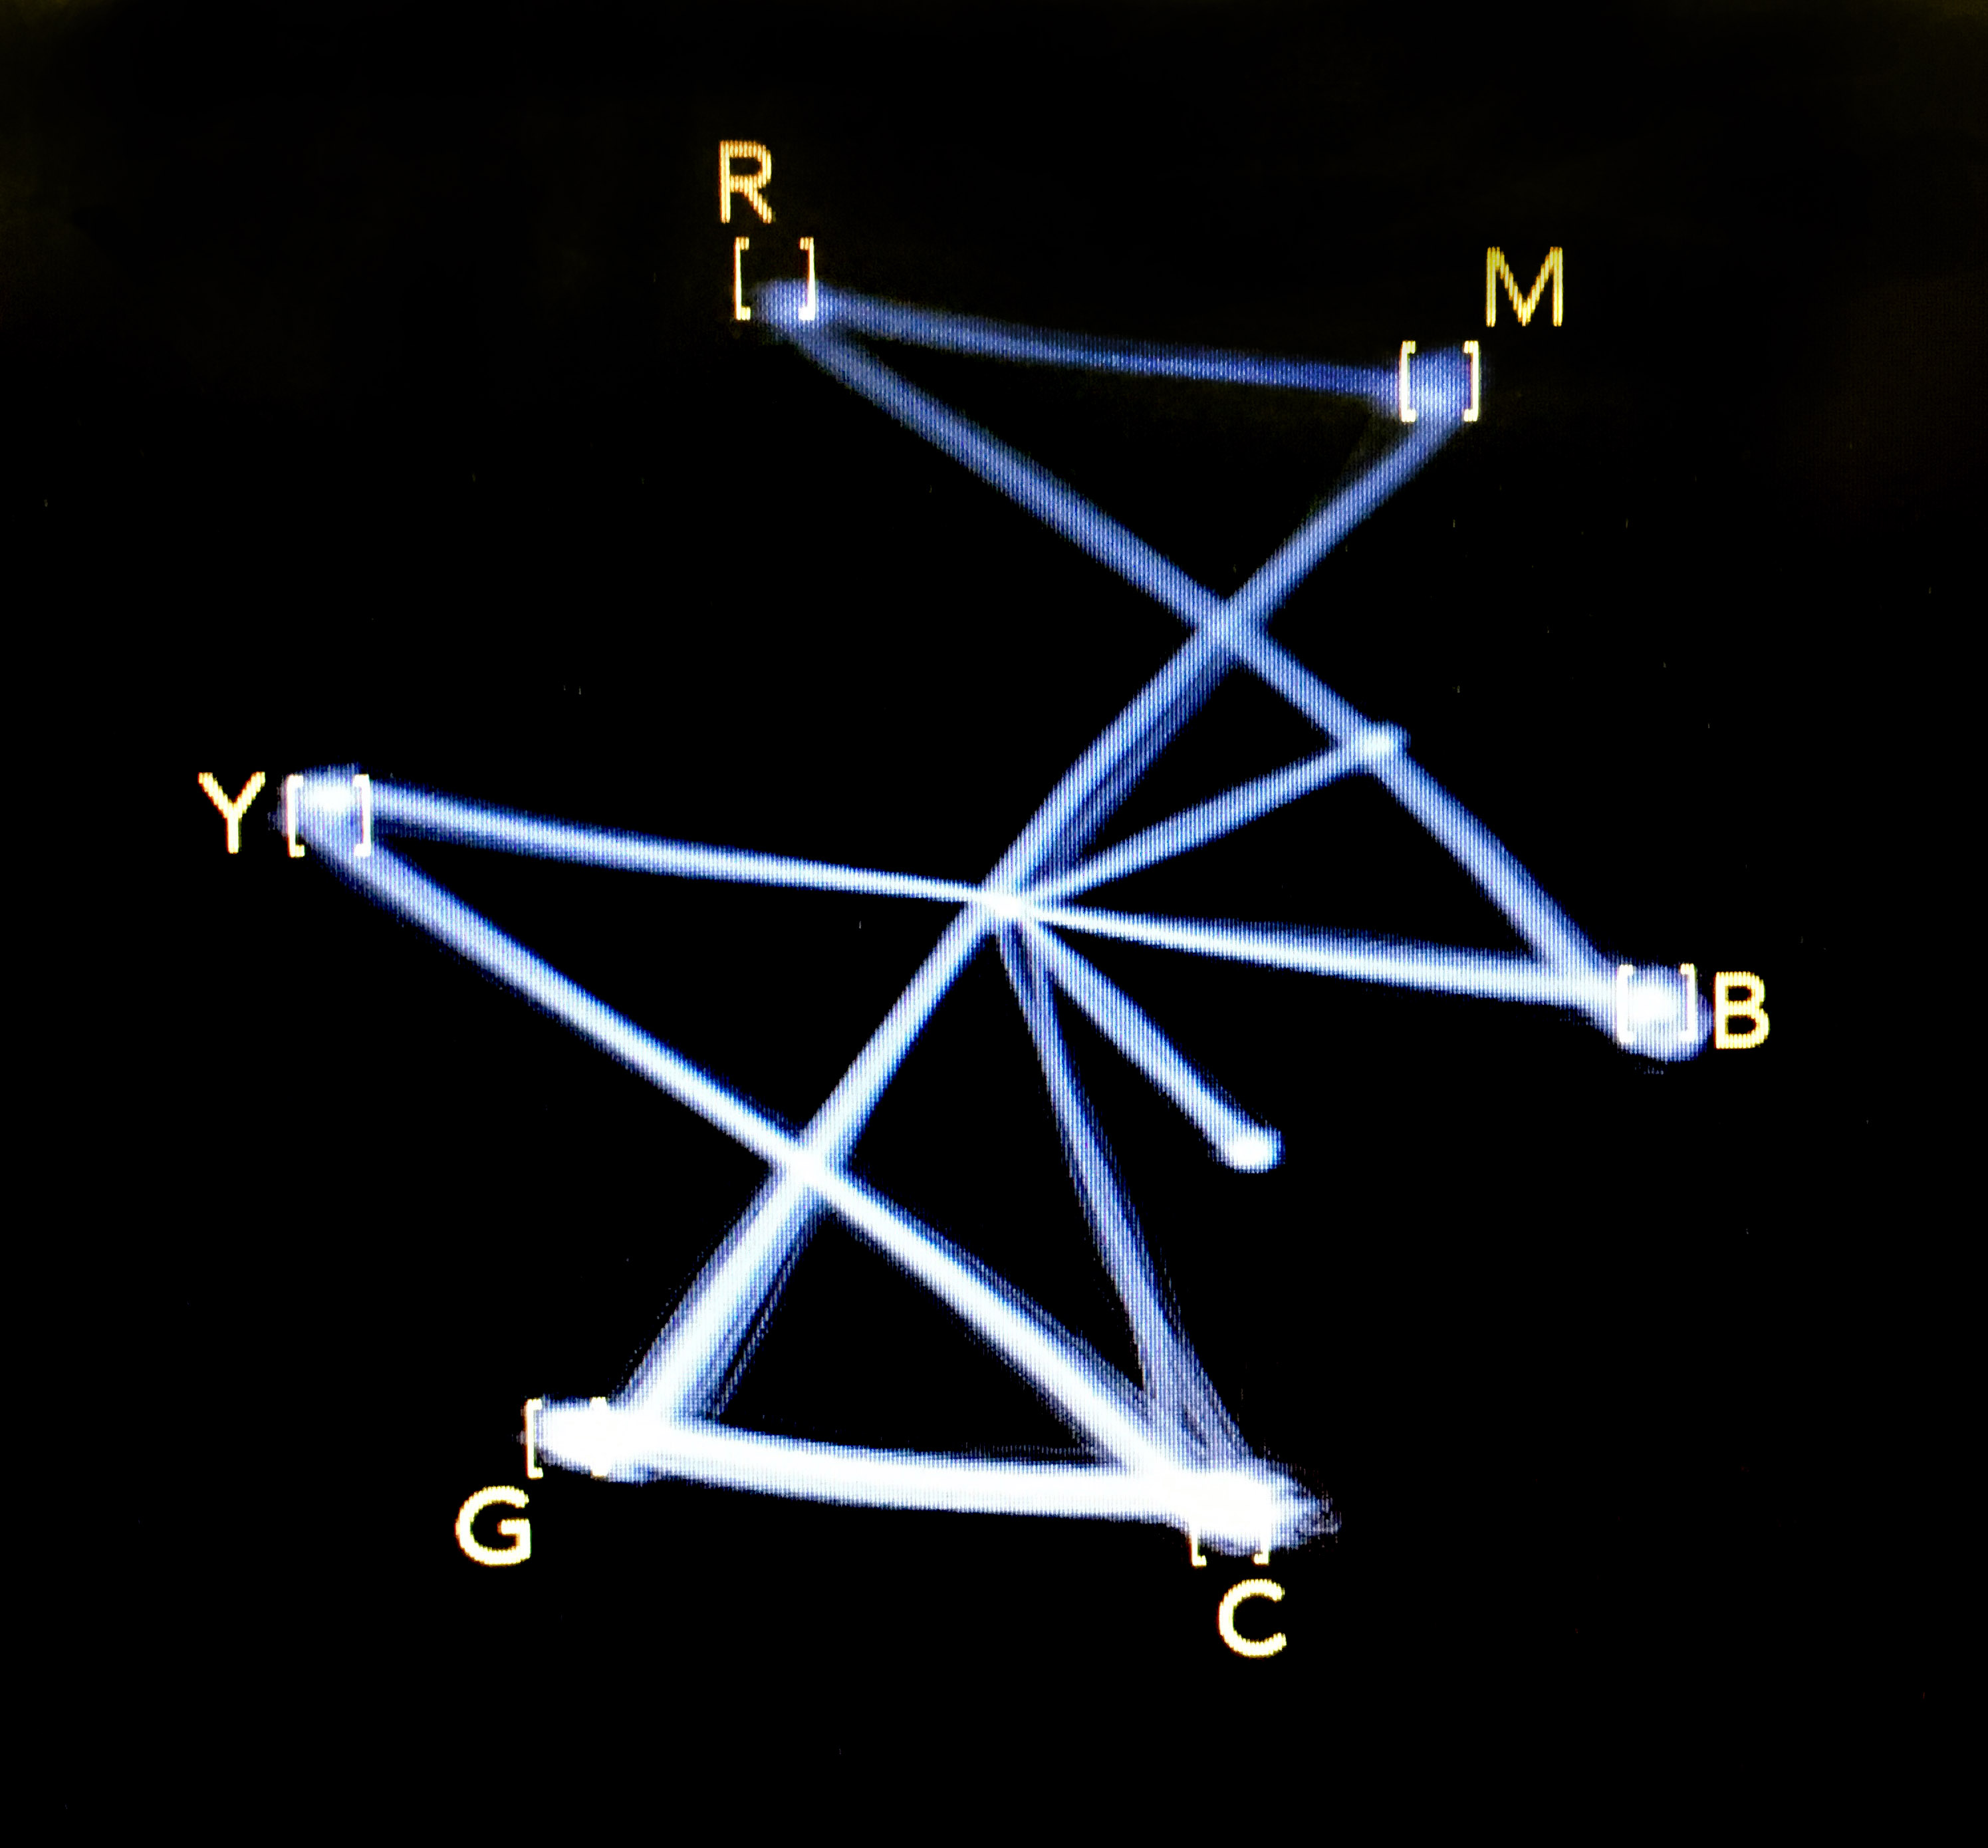
\includegraphics{images/vectorscope.jpg}
\caption{\label{fig:unnamed-chunk-1}Barres de calibration couleur sur vectorscope \citep{marsh_ColorBarsVectorscope_2016}}
\end{figure}

\hypertarget{sources}{%
\section*{Sources}\label{sources}}
\addcontentsline{toc}{section}{Sources}

Compilation via Bookdown \citep{xie_BookdownAuthoringBooks_2020}

\begin{itemize}
\tightlist
\item
  \emph{GIT}\citep{torvalds_Git_2006} hébergé \href{https://github.com/tim-montmorency/543-traitement-video}{github.com/tim-montmorency/543-traitement-video}
\item
  \emph{Libre}\citep{stallman_GnuOrg_1983}
\item
  Écrit en \emph{RMarkdown}\citep{allaire_RmarkdownDynamicDocuments_2020}

  \begin{itemize}
  \tightlist
  \item
    \href{https://tim-montmorency.com/543-traitement-video/}{HTML}
  \item
    \href{https://tim-montmorency.com/543-traitement-video/traitement-video.pdf}{PDF}
  \item
    \href{https://tim-montmorency.com/543-traitement-video/traitement-video.epub}{EPUB}
  \end{itemize}
\item
  \href{https://github.com/tim-montmorency/543-traitement-video/blob/master/582543-traitement-video.bib}{Bibliographie Bibtex}
\end{itemize}

\hypertarget{mo-traitement-viduxe9o}{%
\chapter{582-543-MO Traitement vidéo}\label{mo-traitement-viduxe9o}}

\hypertarget{description-du-cours}{%
\section{Description du cours}\label{description-du-cours}}

\begin{itemize}
\tightlist
\item
  Techniques D'INTÉGRATION MULTIMÉDIA
\item
  Département des techniques d'intégration multimédia
\item
  582.A1
\item
  Pondération : 1-2-2
\item
  Unités: 1,66
\item
  Heures-contact : 45
\item
  Session : 4
\end{itemize}

Ce cours permet à l'étudiante ou l'étudiant d'enregistrer, de modifier et de traiter des images en temps réel.
L'étudiant sera appelé à appliquer des effets visuels aux images vidéo et à adapter les images en fonction de l'intégration.

\hypertarget{objectifs}{%
\section{Objectifs}\label{objectifs}}

\hypertarget{intuxe9grateur-et-ministuxe9riel}{%
\subsection{Intégrateur et ministériel}\label{intuxe9grateur-et-ministuxe9riel}}

\begin{itemize}
\tightlist
\item
  015J Traiter les images en mouvement
\end{itemize}

\hypertarget{apprentissages}{%
\subsection{Apprentissages}\label{apprentissages}}

\begin{itemize}
\tightlist
\item
  Adapter l'image en mouvement (Importance relative\,: 40\% )
\item
  Programmer des effets visuels interactifs (Importance relative\,: 40\% )
\item
  Intégrer l'image en mouvement interactive à une production médiatique (Importance relative\,: 20\% )
\end{itemize}

\hypertarget{pruxe9alables}{%
\section{Préalables}\label{pruxe9alables}}

\hypertarget{pruxe9alable-absolu-au-pruxe9sent-cours}{%
\subsection{Préalable absolu au présent cours~:}\label{pruxe9alable-absolu-au-pruxe9sent-cours}}

\begin{itemize}
\tightlist
\item
  582 413 MO Montage vidéo
\end{itemize}

\hypertarget{pruxe9alable-absolu-aux-cours-suivants}{%
\subsection{Préalable absolu aux cours suivants~:}\label{pruxe9alable-absolu-aux-cours-suivants}}

\begin{itemize}
\tightlist
\item
  582~513 MO Conception de projet multimédia
\item
  582 66B MO Expérience multimédia interactive
\item
  582 66G MO Production Web en entreprise
\end{itemize}

\hypertarget{muxe9thodologie}{%
\section{Méthodologie~}\label{muxe9thodologie}}

L'approche pédagogique de ce cours emprunte à celle employée dans les séminaires de recherche-création en média numérique. Une attention particulière est attribuée au partage de l'expérimentation en lien avec le sujet du cours. Différentes activités pédagogiques seront à l'honneur, notamment :

\begin{itemize}
\tightlist
\item
  Exposés magistraux
\item
  Démonstrations
\item
  Séances de questions
\item
  Présentations étudiantes
\item
  Valorisation des apprentissages autonomes
\item
  Utilisation créative de logiciels
\item
  Travaux pratiques itératifs
\end{itemize}

\hypertarget{duxe9veloppement}{%
\section{Développement}\label{duxe9veloppement}}

\hypertarget{attitudes-professionnelles}{%
\subsection{Attitudes professionnelles}\label{attitudes-professionnelles}}

\begin{itemize}
\tightlist
\item
  Curiosité
\item
  Capacité de partage
\item
  Créativité
\item
  Esprit critique
\item
  Sens esthétique
\end{itemize}

\hypertarget{habiletuxe9s-transdisciplinaires}{%
\subsection{Habiletés transdisciplinaires}\label{habiletuxe9s-transdisciplinaires}}

\begin{itemize}
\tightlist
\item
  Profil \textbf{technologies de l'information et de la communication (TIC)}
\item
  Les étudiantes et étudiants auront à exploiter les TIC de manière efficace et responsable.
\item
  Recherche, traitement et présentation de l'information.
\end{itemize}

\hypertarget{contexte-particulier-dapprentissage}{%
\section{Contexte particulier d'apprentissage}\label{contexte-particulier-dapprentissage}}

\begin{itemize}
\tightlist
\item
  À distance; synchrone.
\item
  Possibilité d'utiliser le laboratoire informatique et le studio si nécessaire.
\end{itemize}

\hypertarget{fiche-technique}{%
\subsection{Fiche technique}\label{fiche-technique}}

\begin{itemize}
\tightlist
\item
  Ordinateurs, projecteurs à haute luminosité ou télévision, haut-parleurs professionnels, casque audio, matériel disponible pour TIM
\item
  Logiciels de montage vidéo et traitemet vidéo en temps réel
\item
  Languages et protocoles de paramétrage\\
\item
  Technicienne ou technicien en travaux pratiques
\end{itemize}

\hypertarget{contenus_essentiels}{%
\section{Contenus essentiels}\label{contenus_essentiels}}

\hypertarget{survol-historique}{%
\subsection{Survol historique}\label{survol-historique}}

\begin{itemize}
\tightlist
\item
  \protect\hyperlink{evolution_historique}{Évolution historique du traitement vidéo dans les différentes formes d'art}

  \begin{itemize}
  \tightlist
  \item
    \protect\hyperlink{evolution_historique_performance}{Performance}
  \item
    \protect\hyperlink{evolution_historique_installation}{Installation}
  \item
    \protect\hyperlink{evolution_historique_technologies}{Évolution des technologies associées}
  \end{itemize}
\item
  \protect\hyperlink{evolution_historique_language}{Langages et moyens expressifs de l'image en mouvement}
\end{itemize}

\hypertarget{fondements-techniques}{%
\subsection{Fondements techniques}\label{fondements-techniques}}

\begin{itemize}
\tightlist
\item
  \protect\hyperlink{lexique_fichiers}{Formats de fichiers}
\item
  \protect\hyperlink{lexique_encodage}{Encodage des vidéos}\\
\item
  \protect\hyperlink{aquerir_captation}{Captation vidéo en temps réel}
\item
  \protect\hyperlink{traiter_logiciels}{Logiciels de traitement vidéo en temps réel et d'interactivité}
\item
  \protect\hyperlink{programmer_logiciels}{Logiciels de programmation nodale}
\item
  Notions de traitement vidéo

  \begin{itemize}
  \tightlist
  \item
    pixels
  \item
    couleurs
  \item
    texture
  \item
    matrice
  \item
    mémoire tampon
  \item
    alpha channel
  \item
    rendu OpenGL
  \end{itemize}
\end{itemize}

\hypertarget{traitement-de-limage-en-mouvement}{%
\subsection{Traitement de l'image en mouvement}\label{traitement-de-limage-en-mouvement}}

\begin{itemize}
\tightlist
\item
  Usage de capture vidéo en temps réel\\
\item
  Effets visuels et filtres applicables en temps réel sur des matériaux visuels\\
\item
  Traitement visuel en temps réel à l'aide d'effets et de logiciels de programmation multimédia et nodale
\item
  Flot de données entre les objets du logiciel
\item
  Exploitation des fonctions des logiciels de traitement vidéo en temps réel
\item
  Utilisation de nuanceurs (shaders)
\end{itemize}

\hypertarget{programmation-deffets-visuels}{%
\subsection{Programmation d'effets visuels}\label{programmation-deffets-visuels}}

\begin{itemize}
\tightlist
\item
  Programmation de compositions visuelles génératives
\item
  Réalisation d'un échantillonneur/mélangeur visuel
\item
  Programmation pour contrôler la lecture vidéo,

  \begin{itemize}
  \tightlist
  \item
    montage temps réel
  \item
    niveau des couleurs
  \item
    alpha channel\\
  \end{itemize}
\item
  Programmation nodale pour créer des effets en temps réel

  \begin{itemize}
  \tightlist
  \item
    position
  \item
    rotation
  \item
    dimensions
  \item
    mixage d'images
  \item
    incrustation
  \item
    distorsion
  \item
    délais
  \item
    rétroaction (feedback)
  \item
    modification de couleurs
  \item
    chromakey
  \item
    lumière
  \item
    fumée
  \item
    texture
  \end{itemize}
\item
  Nuanceurs (shaders)\,: vertex, pixel et géométrie
\end{itemize}

\hypertarget{image-en-mouvement-et-interactivituxe9}{%
\subsection{Image en mouvement et interactivité}\label{image-en-mouvement-et-interactivituxe9}}

\begin{itemize}
\tightlist
\item
  Intégration des composantes dans une production interactive
\item
  Configuration logicielle et matérielle d'une production interactive\\
\item
  Conceptualisation et scénarisation d'un projet visuel interactif\\
\item
  Captation de mouvement et de présence
\item
  Programmation de la captation de mouvement et de présence
\item
  Utilisation d'interfaces de contrôle interactives
\item
  Utilisation d'OSC, MIDI, DMX ou ArtNet pour interagir avec d'autres logiciels et interfaces de contrôle
\end{itemize}

\hypertarget{gestion-de-projets}{%
\subsection{Gestion de projets}\label{gestion-de-projets}}

\begin{itemize}
\tightlist
\item
  Schématisation
\item
  Prototypage
\item
  Gestion de banques d'images
\item
  Optimisation des performances de l'application
\item
  Test de contrôle de qualité
\item
  Préréglages
\item
  Optimisation de la programmation et commentaires
\item
  Console de débogage
\item
  Exportation de projets
\item
  Formats de sauvegarde\\
\item
  Application autonome
\item
  Sauvegarde et archivage des médias
\item
  Ajustement des effets visuels en fonction des tests
\end{itemize}

\hypertarget{calendrier}{%
\chapter{Calendrier}\label{calendrier}}

\href{https://www.cmontmorency.qc.ca/wp-content/uploads/images/college/administration/CALENDRIER-SCOLAIRE-2020-2021.pdf}{Calendrier Collège Montmorency 2020-2021}

\begin{longtable}[]{@{}lll@{}}
\toprule
\begin{minipage}[b]{(\columnwidth - 2\tabcolsep) * \real{0.19}}\raggedright
Séance\strut
\end{minipage} & \begin{minipage}[b]{(\columnwidth - 2\tabcolsep) * \real{0.41}}\raggedright
OBJECTIFS ABORDÉS EN CLASSE\strut
\end{minipage} & \begin{minipage}[b]{(\columnwidth - 2\tabcolsep) * \real{0.41}}\raggedright
ACTIVITÉS AUTONOMES\strut
\end{minipage}\tabularnewline
\midrule
\endhead
\begin{minipage}[t]{(\columnwidth - 2\tabcolsep) * \real{0.19}}\raggedright
\protect\hyperlink{semaine_1}{1;
3
février}\strut
\end{minipage} & \begin{minipage}[t]{(\columnwidth - 2\tabcolsep) * \real{0.41}}\raggedright
Plan de cour;
Survol \protect\hyperlink{corpus}{corpus artistique};
Consignes \protect\hyperlink{sommatif_1}{Présentation corpus
vidéo};\strut
\end{minipage} & \begin{minipage}[t]{(\columnwidth - 2\tabcolsep) * \real{0.41}}\raggedright
Recherche d'un sujet \protect\hyperlink{sommatif_1}{Présentation corpus
vidéo}\strut
\end{minipage}\tabularnewline
\begin{minipage}[t]{(\columnwidth - 2\tabcolsep) * \real{0.19}}\raggedright
\protect\hyperlink{semaine_2}{2;
10
février}\strut
\end{minipage} & \begin{minipage}[t]{(\columnwidth - 2\tabcolsep) * \real{0.41}}\raggedright
\protect\hyperlink{evolution_historique}{Historique du traitement
vidéo};
Formatif Préapprobation \protect\hyperlink{sommatif_1}{Présentation corpus
Vidéo}\strut
\end{minipage} & \begin{minipage}[t]{(\columnwidth - 2\tabcolsep) * \real{0.41}}\raggedright
Préparation \protect\hyperlink{sommatif_1}{Présentation corpus
vidéo}\strut
\end{minipage}\tabularnewline
\begin{minipage}[t]{(\columnwidth - 2\tabcolsep) * \real{0.19}}\raggedright
\protect\hyperlink{semaine_3}{3;
17
février}\strut
\end{minipage} & \begin{minipage}[t]{(\columnwidth - 2\tabcolsep) * \real{0.41}}\raggedright
Sommatif \protect\hyperlink{sommatif_1}{Présentation corpus
Vidéo}\strut
\end{minipage} & \begin{minipage}[t]{(\columnwidth - 2\tabcolsep) * \real{0.41}}\raggedright
\strut
\end{minipage}\tabularnewline
\begin{minipage}[t]{(\columnwidth - 2\tabcolsep) * \real{0.19}}\raggedright
\protect\hyperlink{semaine_4}{4;
24
février}\strut
\end{minipage} & \begin{minipage}[t]{(\columnwidth - 2\tabcolsep) * \real{0.41}}\raggedright
\protect\hyperlink{lexique}{Composantes du signal vidéo};
\protect\hyperlink{acquerir}{Acquérir l'image en mouvement};
\protect\hyperlink{echantillonner}{Échantillonner l'image en
mouvement};
Consignes \protect\hyperlink{sommatif_2}{Question traitement
vidéo}\strut
\end{minipage} & \begin{minipage}[t]{(\columnwidth - 2\tabcolsep) * \real{0.41}}\raggedright
Préparation \protect\hyperlink{sommatif_2}{Question traitement
vidéo}\strut
\end{minipage}\tabularnewline
\begin{minipage}[t]{(\columnwidth - 2\tabcolsep) * \real{0.19}}\raggedright
\protect\hyperlink{semaine_5}{X;
3
mars}\strut
\end{minipage} & \begin{minipage}[t]{(\columnwidth - 2\tabcolsep) * \real{0.41}}\raggedright
Journées de rattrapage (Pas de cours)\strut
\end{minipage} & \begin{minipage}[t]{(\columnwidth - 2\tabcolsep) * \real{0.41}}\raggedright
\strut
\end{minipage}\tabularnewline
\begin{minipage}[t]{(\columnwidth - 2\tabcolsep) * \real{0.19}}\raggedright
\protect\hyperlink{semaine_6}{5;
10
mars}\strut
\end{minipage} & \begin{minipage}[t]{(\columnwidth - 2\tabcolsep) * \real{0.41}}\raggedright
\protect\hyperlink{traiter}{Traiter l'image en mouvement};
Formatif Préapprobation \protect\hyperlink{sommatif_2}{Question traitement
vidéo}\strut
\end{minipage} & \begin{minipage}[t]{(\columnwidth - 2\tabcolsep) * \real{0.41}}\raggedright
Soumettre \protect\hyperlink{sommatif_2}{Question traitement
vidéo}\strut
\end{minipage}\tabularnewline
\begin{minipage}[t]{(\columnwidth - 2\tabcolsep) * \real{0.19}}\raggedright
\protect\hyperlink{semaine_7}{6;
17
mars}\strut
\end{minipage} & \begin{minipage}[t]{(\columnwidth - 2\tabcolsep) * \real{0.41}}\raggedright
Consignes \protect\hyperlink{sommatif_4}{Palette vidéo
interactive};
Sommatif \protect\hyperlink{sommatif_3}{Quiz traitement vidéo}\strut
\end{minipage} & \begin{minipage}[t]{(\columnwidth - 2\tabcolsep) * \real{0.41}}\raggedright
Préparation \protect\hyperlink{sommatif_4}{Palette vidéo
interactive}\strut
\end{minipage}\tabularnewline
\begin{minipage}[t]{(\columnwidth - 2\tabcolsep) * \real{0.19}}\raggedright
\protect\hyperlink{semaine_8}{7;
24
mars}\strut
\end{minipage} & \begin{minipage}[t]{(\columnwidth - 2\tabcolsep) * \real{0.41}}\raggedright
\protect\hyperlink{programmer}{Programmer des sources visuelles}\strut
\end{minipage} & \begin{minipage}[t]{(\columnwidth - 2\tabcolsep) * \real{0.41}}\raggedright
Préparation \protect\hyperlink{sommatif_4}{Palette vidéo
interactive}\strut
\end{minipage}\tabularnewline
\begin{minipage}[t]{(\columnwidth - 2\tabcolsep) * \real{0.19}}\raggedright
\protect\hyperlink{semaine_9}{8;
31
mars}\strut
\end{minipage} & \begin{minipage}[t]{(\columnwidth - 2\tabcolsep) * \real{0.41}}\raggedright
\protect\hyperlink{interagir}{Interagir avec des sources vidéo}\strut
\end{minipage} & \begin{minipage}[t]{(\columnwidth - 2\tabcolsep) * \real{0.41}}\raggedright
Préparation \protect\hyperlink{sommatif_4}{Palette vidéo
interactive}\strut
\end{minipage}\tabularnewline
\begin{minipage}[t]{(\columnwidth - 2\tabcolsep) * \real{0.19}}\raggedright
\protect\hyperlink{semaine_10}{X;
7
avril}\strut
\end{minipage} & \begin{minipage}[t]{(\columnwidth - 2\tabcolsep) * \real{0.41}}\raggedright
Congé (Pas de cours)\strut
\end{minipage} & \begin{minipage}[t]{(\columnwidth - 2\tabcolsep) * \real{0.41}}\raggedright
\strut
\end{minipage}\tabularnewline
\begin{minipage}[t]{(\columnwidth - 2\tabcolsep) * \real{0.19}}\raggedright
\protect\hyperlink{semaine_11}{9;
14
avril}\strut
\end{minipage} & \begin{minipage}[t]{(\columnwidth - 2\tabcolsep) * \real{0.41}}\raggedright
Suite \protect\hyperlink{programmer}{Programmer des sources
visuelles};
et \protect\hyperlink{interagir}{Interagir avec des sources
vidéo}\strut
\end{minipage} & \begin{minipage}[t]{(\columnwidth - 2\tabcolsep) * \real{0.41}}\raggedright
Préparation \protect\hyperlink{sommatif_4}{Palette vidéo
interactive}\strut
\end{minipage}\tabularnewline
\begin{minipage}[t]{(\columnwidth - 2\tabcolsep) * \real{0.19}}\raggedright
\protect\hyperlink{semaine_12}{10;
21
avril}\strut
\end{minipage} & \begin{minipage}[t]{(\columnwidth - 2\tabcolsep) * \real{0.41}}\raggedright
Sommatif \protect\hyperlink{sommatif_4}{Palette vidéo
interactive}\strut
\end{minipage} & \begin{minipage}[t]{(\columnwidth - 2\tabcolsep) * \real{0.41}}\raggedright
\strut
\end{minipage}\tabularnewline
\begin{minipage}[t]{(\columnwidth - 2\tabcolsep) * \real{0.19}}\raggedright
\protect\hyperlink{semaine_13}{11;
28
avril}\strut
\end{minipage} & \begin{minipage}[t]{(\columnwidth - 2\tabcolsep) * \real{0.41}}\raggedright
\protect\hyperlink{deployer}{Déployer un projet vidéo temps
réel};
Consignes \protect\hyperlink{sommatif_5}{performance audiovisuelle temps
réel}\strut
\end{minipage} & \begin{minipage}[t]{(\columnwidth - 2\tabcolsep) * \real{0.41}}\raggedright
Préparation \protect\hyperlink{sommatif_5}{performance audiovisuelle temps
réel}\strut
\end{minipage}\tabularnewline
\begin{minipage}[t]{(\columnwidth - 2\tabcolsep) * \real{0.19}}\raggedright
\protect\hyperlink{semaine_14}{12;
5
mai}\strut
\end{minipage} & \begin{minipage}[t]{(\columnwidth - 2\tabcolsep) * \real{0.41}}\raggedright
Suite \protect\hyperlink{deployer}{Déployer un projet vidéo temps
réel}\strut
\end{minipage} & \begin{minipage}[t]{(\columnwidth - 2\tabcolsep) * \real{0.41}}\raggedright
Préparation \protect\hyperlink{sommatif_5}{performance audiovisuelle temps
réel}\strut
\end{minipage}\tabularnewline
\begin{minipage}[t]{(\columnwidth - 2\tabcolsep) * \real{0.19}}\raggedright
\protect\hyperlink{semaine_15}{13;
12
mai}\strut
\end{minipage} & \begin{minipage}[t]{(\columnwidth - 2\tabcolsep) * \real{0.41}}\raggedright
Préparation \protect\hyperlink{sommatif_5}{performance audiovisuelle temps
réel}\strut
\end{minipage} & \begin{minipage}[t]{(\columnwidth - 2\tabcolsep) * \real{0.41}}\raggedright
Préparation \protect\hyperlink{sommatif_5}{performance audiovisuelle temps
réel}\strut
\end{minipage}\tabularnewline
\begin{minipage}[t]{(\columnwidth - 2\tabcolsep) * \real{0.19}}\raggedright
\protect\hyperlink{semaine_16}{14;
18
mai}\strut
\end{minipage} & \begin{minipage}[t]{(\columnwidth - 2\tabcolsep) * \real{0.41}}\raggedright
Exceptionnellement un mardi,
\protect\hyperlink{sommatif_5}{performance audiovisuelle temps
réel};\strut
\end{minipage} & \begin{minipage}[t]{(\columnwidth - 2\tabcolsep) * \real{0.41}}\raggedright
Rédaction du document accompagnateur
\protect\hyperlink{sommatif_5}{performance audiovisuelle temps réel}\strut
\end{minipage}\tabularnewline
\begin{minipage}[t]{(\columnwidth - 2\tabcolsep) * \real{0.19}}\raggedright
\protect\hyperlink{semaine_17}{X;
19
mai}\strut
\end{minipage} & \begin{minipage}[t]{(\columnwidth - 2\tabcolsep) * \real{0.41}}\raggedright
Épreuve uniforme de français (Pas de cours)\strut
\end{minipage} & \begin{minipage}[t]{(\columnwidth - 2\tabcolsep) * \real{0.41}}\raggedright
Rédaction document \protect\hyperlink{sommatif_5}{performance audiovisuelle
temps réel}\strut
\end{minipage}\tabularnewline
\begin{minipage}[t]{(\columnwidth - 2\tabcolsep) * \real{0.19}}\raggedright
\protect\hyperlink{semaine_18}{15;
25
mai}\strut
\end{minipage} & \begin{minipage}[t]{(\columnwidth - 2\tabcolsep) * \real{0.41}}\raggedright
Remise du document accompagnateur \protect\hyperlink{sommatif_5}{performance
audiovisuelle temps réel}\strut
\end{minipage} & \begin{minipage}[t]{(\columnwidth - 2\tabcolsep) * \real{0.41}}\raggedright
\strut
\end{minipage}\tabularnewline
\bottomrule
\end{longtable}

\hypertarget{semaine_1}{%
\section{\texorpdfstring{Séance \protect\hyperlink{semaine_1}{1; 3 février}}{Séance 1; 3 février}}\label{semaine_1}}

\hypertarget{objectifs-aborduxe9s-en-classe}{%
\subsection{OBJECTIFS ABORDÉS EN CLASSE}\label{objectifs-aborduxe9s-en-classe}}

Plan de cour
Survol \protect\hyperlink{corpus}{corpus artistique}
Consignes \protect\hyperlink{sommatif_1}{Présentation corpus vidéo}

\hypertarget{activituxe9s-autonomes}{%
\subsection{ACTIVITÉS AUTONOMES}\label{activituxe9s-autonomes}}

Recherche d'un sujet \protect\hyperlink{sommatif_1}{Présentation corpus vidéo}

\hypertarget{semaine_2}{%
\section{\texorpdfstring{Séance \protect\hyperlink{semaine_2}{2; 10 février}}{Séance 2; 10 février}}\label{semaine_2}}

\hypertarget{objectifs-aborduxe9s-en-classe-1}{%
\subsection{OBJECTIFS ABORDÉS EN CLASSE}\label{objectifs-aborduxe9s-en-classe-1}}

\protect\hyperlink{evolution_historique}{Historique du traitement vidéo}
Formatif Préapprobation \protect\hyperlink{sommatif_1}{Présentation corpus Vidéo}

\hypertarget{activituxe9s-autonomes-1}{%
\subsection{ACTIVITÉS AUTONOMES}\label{activituxe9s-autonomes-1}}

Préparation \protect\hyperlink{sommatif_1}{Présentation corpus vidéo}

\hypertarget{semaine_3}{%
\section{\texorpdfstring{Séance \protect\hyperlink{semaine_3}{3; 17 février}}{Séance 3; 17 février}}\label{semaine_3}}

\hypertarget{objectifs-aborduxe9s-en-classe-2}{%
\subsection{OBJECTIFS ABORDÉS EN CLASSE}\label{objectifs-aborduxe9s-en-classe-2}}

Sommatif \protect\hyperlink{sommatif_1}{Présentation corpus Vidéo}

\hypertarget{activituxe9s-autonomes-2}{%
\subsection{ACTIVITÉS AUTONOMES}\label{activituxe9s-autonomes-2}}

\hypertarget{semaine_4}{%
\section{\texorpdfstring{Séance \protect\hyperlink{semaine_4}{4; 24 février}}{Séance 4; 24 février}}\label{semaine_4}}

\hypertarget{objectifs-aborduxe9s-en-classe-3}{%
\subsection{OBJECTIFS ABORDÉS EN CLASSE}\label{objectifs-aborduxe9s-en-classe-3}}

\protect\hyperlink{lexique}{Composantes du signal vidéo}
\protect\hyperlink{acquerir}{Acquérir l'image en mouvement}
\protect\hyperlink{echantillonner}{Échantillonner l'image en mouvement}
Consignes \protect\hyperlink{sommatif_2}{Question traitement vidéo}

\hypertarget{activituxe9s-autonomes-3}{%
\subsection{ACTIVITÉS AUTONOMES}\label{activituxe9s-autonomes-3}}

Préparation \protect\hyperlink{sommatif_2}{Question traitement vidéo}

\hypertarget{semaine_5}{%
\section{\texorpdfstring{Séance \protect\hyperlink{semaine_5}{X; 3 mars}}{Séance X; 3 mars}}\label{semaine_5}}

\hypertarget{objectifs-aborduxe9s-en-classe-4}{%
\subsection{OBJECTIFS ABORDÉS EN CLASSE}\label{objectifs-aborduxe9s-en-classe-4}}

Journées de rattrapage (Pas de cours)

\hypertarget{activituxe9s-autonomes-4}{%
\subsection{ACTIVITÉS AUTONOMES}\label{activituxe9s-autonomes-4}}

\hypertarget{semaine_6}{%
\section{\texorpdfstring{Séance \protect\hyperlink{semaine_6}{5; 10 mars}}{Séance 5; 10 mars}}\label{semaine_6}}

\hypertarget{objectifs-aborduxe9s-en-classe-5}{%
\subsection{OBJECTIFS ABORDÉS EN CLASSE}\label{objectifs-aborduxe9s-en-classe-5}}

\protect\hyperlink{traiter}{Traiter l'image en mouvement}
Formatif Préapprobation \protect\hyperlink{sommatif_2}{Question traitement vidéo}

\hypertarget{activituxe9s-autonomes-5}{%
\subsection{ACTIVITÉS AUTONOMES}\label{activituxe9s-autonomes-5}}

Soumettre \protect\hyperlink{sommatif_2}{Question traitement vidéo}

\hypertarget{semaine_7}{%
\section{\texorpdfstring{Séance \protect\hyperlink{semaine_7}{6; 17 mars}}{Séance 6; 17 mars}}\label{semaine_7}}

\hypertarget{objectifs-aborduxe9s-en-classe-6}{%
\subsection{OBJECTIFS ABORDÉS EN CLASSE}\label{objectifs-aborduxe9s-en-classe-6}}

Consignes \protect\hyperlink{sommatif_4}{Palette vidéo interactive}
Sommatif \protect\hyperlink{sommatif_3}{Quiz traitement vidéo}

\hypertarget{activituxe9s-autonomes-6}{%
\subsection{ACTIVITÉS AUTONOMES}\label{activituxe9s-autonomes-6}}

Préparation \protect\hyperlink{sommatif_4}{Palette vidéo interactive}

\hypertarget{semaine_8}{%
\section{\texorpdfstring{Séance \protect\hyperlink{semaine_8}{7; 24 mars}}{Séance 7; 24 mars}}\label{semaine_8}}

\hypertarget{objectifs-aborduxe9s-en-classe-7}{%
\subsection{OBJECTIFS ABORDÉS EN CLASSE}\label{objectifs-aborduxe9s-en-classe-7}}

\protect\hyperlink{programmer}{Programmer des sources visuelles}

\hypertarget{activituxe9s-autonomes-7}{%
\subsection{ACTIVITÉS AUTONOMES}\label{activituxe9s-autonomes-7}}

Préparation \protect\hyperlink{sommatif_4}{Palette vidéo interactive}

\hypertarget{semaine_9}{%
\section{\texorpdfstring{Séance \protect\hyperlink{semaine_9}{8; 31 mars}}{Séance 8; 31 mars}}\label{semaine_9}}

\hypertarget{objectifs-aborduxe9s-en-classe-8}{%
\subsection{OBJECTIFS ABORDÉS EN CLASSE}\label{objectifs-aborduxe9s-en-classe-8}}

\protect\hyperlink{interagir}{Interagir avec des sources vidéo}

\hypertarget{activituxe9s-autonomes-8}{%
\subsection{ACTIVITÉS AUTONOMES}\label{activituxe9s-autonomes-8}}

Préparation \protect\hyperlink{sommatif_4}{Palette vidéo interactive}

\hypertarget{semaine_10}{%
\section{\texorpdfstring{Séance \protect\hyperlink{semaine_10}{X; 7 avril}}{Séance X; 7 avril}}\label{semaine_10}}

\hypertarget{objectifs-aborduxe9s-en-classe-9}{%
\subsection{OBJECTIFS ABORDÉS EN CLASSE}\label{objectifs-aborduxe9s-en-classe-9}}

Congé (Pas de cours)

\hypertarget{activituxe9s-autonomes-9}{%
\subsection{ACTIVITÉS AUTONOMES}\label{activituxe9s-autonomes-9}}

\hypertarget{semaine_11}{%
\section{\texorpdfstring{Séance \protect\hyperlink{semaine_11}{9; 14 avril}}{Séance 9; 14 avril}}\label{semaine_11}}

\hypertarget{objectifs-aborduxe9s-en-classe-10}{%
\subsection{OBJECTIFS ABORDÉS EN CLASSE}\label{objectifs-aborduxe9s-en-classe-10}}

Suite \protect\hyperlink{programmer}{Programmer des sources visuelles}
et \protect\hyperlink{interagir}{Interagir avec des sources vidéo}

\hypertarget{activituxe9s-autonomes-10}{%
\subsection{ACTIVITÉS AUTONOMES}\label{activituxe9s-autonomes-10}}

Préparation \protect\hyperlink{sommatif_4}{Palette vidéo interactive}

\hypertarget{semaine_12}{%
\section{\texorpdfstring{Séance \protect\hyperlink{semaine_12}{10; 21 avril}}{Séance 10; 21 avril}}\label{semaine_12}}

\hypertarget{objectifs-aborduxe9s-en-classe-11}{%
\subsection{OBJECTIFS ABORDÉS EN CLASSE}\label{objectifs-aborduxe9s-en-classe-11}}

Sommatif \protect\hyperlink{sommatif_4}{Palette vidéo interactive}

\hypertarget{activituxe9s-autonomes-11}{%
\subsection{ACTIVITÉS AUTONOMES}\label{activituxe9s-autonomes-11}}

\hypertarget{semaine_13}{%
\section{\texorpdfstring{Séance \protect\hyperlink{semaine_13}{11; 28 avril}}{Séance 11; 28 avril}}\label{semaine_13}}

\hypertarget{objectifs-aborduxe9s-en-classe-12}{%
\subsection{OBJECTIFS ABORDÉS EN CLASSE}\label{objectifs-aborduxe9s-en-classe-12}}

\protect\hyperlink{deployer}{Déployer un projet vidéo temps réel}
Consignes \protect\hyperlink{sommatif_5}{performance audiovisuelle temps réel}

\hypertarget{activituxe9s-autonomes-12}{%
\subsection{ACTIVITÉS AUTONOMES}\label{activituxe9s-autonomes-12}}

Préparation \protect\hyperlink{sommatif_5}{performance audiovisuelle temps réel}

\hypertarget{semaine_14}{%
\section{\texorpdfstring{Séance \protect\hyperlink{semaine_14}{12; 5 mai}}{Séance 12; 5 mai}}\label{semaine_14}}

\hypertarget{objectifs-aborduxe9s-en-classe-13}{%
\subsection{OBJECTIFS ABORDÉS EN CLASSE}\label{objectifs-aborduxe9s-en-classe-13}}

Suite \protect\hyperlink{deployer}{Déployer un projet vidéo temps réel}

\hypertarget{activituxe9s-autonomes-13}{%
\subsection{ACTIVITÉS AUTONOMES}\label{activituxe9s-autonomes-13}}

Préparation \protect\hyperlink{sommatif_5}{performance audiovisuelle temps réel}

\hypertarget{semaine_15}{%
\section{\texorpdfstring{Séance \protect\hyperlink{semaine_15}{13; 12 mai}}{Séance 13; 12 mai}}\label{semaine_15}}

\hypertarget{objectifs-aborduxe9s-en-classe-14}{%
\subsection{OBJECTIFS ABORDÉS EN CLASSE}\label{objectifs-aborduxe9s-en-classe-14}}

Préparation \protect\hyperlink{sommatif_5}{performance audiovisuelle temps réel}

\hypertarget{activituxe9s-autonomes-14}{%
\subsection{ACTIVITÉS AUTONOMES}\label{activituxe9s-autonomes-14}}

Préparation \protect\hyperlink{sommatif_5}{performance audiovisuelle temps réel}

\hypertarget{semaine_16}{%
\section{\texorpdfstring{Séance \protect\hyperlink{semaine_16}{14; 18 mai}}{Séance 14; 18 mai}}\label{semaine_16}}

\hypertarget{objectifs-aborduxe9s-en-classe-15}{%
\subsection{OBJECTIFS ABORDÉS EN CLASSE}\label{objectifs-aborduxe9s-en-classe-15}}

Exceptionnellement un mardi,
\protect\hyperlink{sommatif_5}{performance audiovisuelle temps réel}

\hypertarget{activituxe9s-autonomes-15}{%
\subsection{ACTIVITÉS AUTONOMES}\label{activituxe9s-autonomes-15}}

Rédaction du document accompagnateur \protect\hyperlink{sommatif_5}{performance audiovisuelle temps réel}

\hypertarget{semaine_17}{%
\section{\texorpdfstring{Séance \protect\hyperlink{semaine_17}{X; 19 mai}}{Séance X; 19 mai}}\label{semaine_17}}

\hypertarget{objectifs-aborduxe9s-en-classe-16}{%
\subsection{OBJECTIFS ABORDÉS EN CLASSE}\label{objectifs-aborduxe9s-en-classe-16}}

Épreuve uniforme de français (Pas de cours)

\hypertarget{activituxe9s-autonomes-16}{%
\subsection{ACTIVITÉS AUTONOMES}\label{activituxe9s-autonomes-16}}

Rédaction document \protect\hyperlink{sommatif_5}{performance audiovisuelle temps réel}

\hypertarget{semaine_18}{%
\section{\texorpdfstring{Séance \protect\hyperlink{semaine_18}{15; 25 mai}}{Séance 15; 25 mai}}\label{semaine_18}}

\hypertarget{objectifs-aborduxe9s-en-classe-17}{%
\subsection{OBJECTIFS ABORDÉS EN CLASSE}\label{objectifs-aborduxe9s-en-classe-17}}

Remise du document accompagnateur \protect\hyperlink{sommatif_5}{performance audiovisuelle temps réel}

\hypertarget{activituxe9s-autonomes-17}{%
\subsection{ACTIVITÉS AUTONOMES}\label{activituxe9s-autonomes-17}}

\hypertarget{exercices}{%
\chapter{Exercices}\label{exercices}}

\hypertarget{sommatif_1}{%
\section{Présentation corpus vidéo}\label{sommatif_1}}

\begin{itemize}
\tightlist
\item
  Présentation de type partage d'écran de \textasciitilde5 minutes
\item
  Sommatif (15\%)
\item
  Individuel
\end{itemize}

\hypertarget{consignes}{%
\subsection{Consignes}\label{consignes}}

\begin{itemize}
\tightlist
\item
  Choisir et présenter un court extrait médiatique comprenant un procédé de traitement vidéo original

  \begin{itemize}
  \tightlist
  \item
    Se référer à la section \protect\hyperlink{corpus}{corpus} pour une liste d'artistes potentiellement inspirants
  \end{itemize}
\item
  Présentez visuellement les informations suivantes

  \begin{itemize}
  \tightlist
  \item
    Contextualisation historique écrite de l'auteur comprenant

    \begin{itemize}
    \tightlist
    \item
      Nom,
    \item
      année de naissance (si disponible) et décès (si disponible)
    \item
      nationalité (ville, pays (si disponible)),
    \item
      ex; personne vivante:
    \end{itemize}

\begin{Shaded}
\begin{Highlighting}[]
\NormalTok{Marina Abramovic, 1946 à Belgrade, Yougoslavie (aujourd\textquotesingle{}hui Serbie{-}Monténégro)}
\end{Highlighting}
\end{Shaded}

    \begin{itemize}
    \tightlist
    \item
      ex; personne décédée:
    \end{itemize}

\begin{Shaded}
\begin{Highlighting}[]
\NormalTok{Marcel Duchamp, 1887 à Blainville{-}Crevon (France), et mort le 2 octobre 1968 à Neuilly{-}sur{-}Seine (France).}
\end{Highlighting}
\end{Shaded}
  \item
    Présenter un ou des extraits visuels
  \item
    Contexte de diffusion de l'oeuvre

    \begin{itemize}
    \tightlist
    \item
      Titre

      \begin{itemize}
      \tightlist
      \item
        ex. Twenty four hour Psycho
      \end{itemize}
    \item
      médium, durée, date de parution

      \begin{itemize}
      \tightlist
      \item
        ex. Installation vidéo à 6 canaux, couleur, son, 12 minutes, 1997
      \end{itemize}
    \end{itemize}
  \end{itemize}
\item
  Décrire une technique de traitement vidéo employée

  \begin{itemize}
  \tightlist
  \item
    Ex. La chronophotographie (décrire la technique) fut employé pour (décrire une motivation artistique)
  \end{itemize}
\item
  Présenter une hypothèse à la question suivante :

  \begin{itemize}
  \tightlist
  \item
    Est-ce que ce procédé de traitement vidéo étudié pourrait être produit en temps réel?

    \begin{itemize}
    \tightlist
    \item
      si oui, comment?
    \item
      sinon, pourquoi?
    \end{itemize}
  \end{itemize}
\end{itemize}

\hypertarget{sommatif_2}{%
\section{Rédaction d'une question portant sur le traitement vidéo}\label{sommatif_2}}

\begin{itemize}
\tightlist
\item
  Rédaction dans un tableur en ligne

  \begin{itemize}
  \tightlist
  \item
    Une question portant sur le traitement vidéo
  \item
    Une bonne réponse
  \item
    Trois réponses erronées\\
  \end{itemize}
\item
  Sommatif (10\%)
\item
  Individuel
\end{itemize}

\hypertarget{ex.-question-sur-le-traitement}{%
\subsection{Ex. question sur le traitement,}\label{ex.-question-sur-le-traitement}}

q: Quel type de traitement d'incrustation d'image
x:
b:
c:
d:

\hypertarget{consignes-1}{%
\subsection{Consignes}\label{consignes-1}}

\begin{itemize}
\tightlist
\item
  Rédiger une question pertinente et originale sur le traitement vidéo
\item
  Inscrire une réponse adéquate
\item
  Inventer trois réponses erronées (formatif)
\item
  Se référer aux \href{}{contenus essentiels}
\end{itemize}

\hypertarget{sommatif_3}{%
\section{Jeu-questionnaire théorique}\label{sommatif_3}}

\begin{itemize}
\tightlist
\item
  Formulaire en ligne à répondre avant la date prévue
\item
  Sommatif (15\%)
\item
  Individuel
\end{itemize}

\hypertarget{consignes-2}{%
\subsection{Consignes}\label{consignes-2}}

\begin{itemize}
\tightlist
\item
  Répondre aux questions dans le formulaire avant l'échéance
\end{itemize}

\hypertarget{sommatif_4}{%
\section{Palette de scènes vidéo interactives}\label{sommatif_4}}

\begin{itemize}
\tightlist
\item
  Présentation de type partage d'écran \textasciitilde5 minutes
\item
  Sommatif 25\%
\item
  individuel
\end{itemize}

\hypertarget{consignes-3}{%
\subsection{Consignes}\label{consignes-3}}

\begin{itemize}
\tightlist
\item
  Assembler une palette de 8 scènes vidéo comprenant

  \begin{itemize}
  \tightlist
  \item
    échantillons vidéo
  \item
    caméra vidéo
  \item
    source HTML
  \item
    source nuancier
  \item
    etc.
  \end{itemize}
\item
  Démontrer

  \begin{itemize}
  \tightlist
  \item
    Capacité d'adapter l'image en mouvement
  \item
    Capacité d'interagir avec des effets visuels interactifs
  \item
    Maitrise technique
  \item
    Créativité
  \end{itemize}
\item
  Peut définitivement s'inspirer de la formule dérapage :

  \begin{itemize}
  \tightlist
  \item
    \url{https://derapage.ca/?fbclid=IwAR1VeYPaM7V9x1IoA0_eM9vtRQpD9VERCpwDl4oRTxOXK_n41Vol67EQH5E}
  \end{itemize}
\end{itemize}

\hypertarget{sommatif_5}{%
\section{Performance audiovisuelle temps réel et document accompagnateur}\label{sommatif_5}}

\begin{itemize}
\tightlist
\item
  35\% individuel, produit en équipe
\item
  Présentation courte au sein d'une diffusion audiovisuelle continue (Stream)
\item
  Présenté lors de la ruche u
\item
  Signal issu d'un processus de mélange de signaux en temps réel
\item
  Variation en temps réel de paramètres vidéo programmés
\end{itemize}

\hypertarget{consignes-4}{%
\subsection{Consignes}\label{consignes-4}}

\hypertarget{performance-audiovisuelle-temps-ruxe9el}{%
\subsubsection{Performance audiovisuelle temps réel}\label{performance-audiovisuelle-temps-ruxe9el}}

\begin{itemize}
\tightlist
\item
  Activité concertée avec le cours de Conception sonore interactive
\item
  le traitement vidéo doit être effectué en temps réel
\item
  Présentation de type streaming lors de la ruche (mardi)
\item
  Tous les groupes doivent diffuser ce jour-là
\end{itemize}

\hypertarget{consignes-document-accompagnateur}{%
\subsubsection{Consignes (document accompagnateur}\label{consignes-document-accompagnateur}}

\begin{itemize}
\tightlist
\item
  Remise avant le 26 mai d'un texte individuel expliquant dans un langage approprié et précis les éléments suivant:

  \begin{itemize}
  \tightlist
  \item
    L'implication au sein du projet
  \item
    Les intentions artistiques
  \item
    Les défis techniques
  \item
    La démarche
  \item
    L'inspiration
  \item
    Le fonctionnement technique du travail
  \item
    Ce qui aurait pu améliorer le résultat
  \end{itemize}
\item
  N.B. : un document par étudiant, soumis à la fois au cours de Traitement vidéo ainsi qu'au cours de Conception sonore interactive. Seuls les éléments décrits dans ce texte compteront à l'évaluation. Ne pas oublier de détailler autant l'aspect visuel que le sonore.
\end{itemize}

\hypertarget{corpus}{%
\chapter{Corpus d'art vidéo}\label{corpus}}

(non exaustif bien sur)

\hypertarget{les-origines}{%
\section{Les origines}\label{les-origines}}

\hypertarget{eadward-muybridge}{%
\section{Eadward Muybridge}\label{eadward-muybridge}}

\begin{figure}
\centering
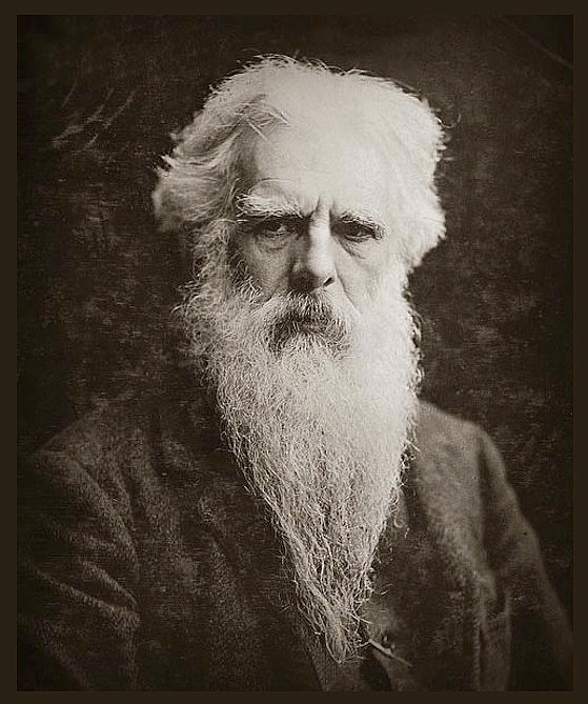
\includegraphics[width=0.5\textwidth,height=\textheight]{medias/corpus/muybridge/Optic_Projection_fig_411.jpg}
\caption{Eadward Muybridge (1830-1904)}
\end{figure}

\begin{figure}
\centering
\includegraphics[width=0.5\textwidth,height=\textheight]{medias/corpus/muybridge/Zoopraxiscope_16485d.gif}
\caption{Zoopraxiscope, 1893}
\end{figure}

\begin{figure}
\centering
\includegraphics[width=0.5\textwidth,height=\textheight]{medias/corpus/muybridge/Phenakistoscope.gif}
\caption{Phénakistiscope, 1893}
\end{figure}

\begin{figure}
\centering
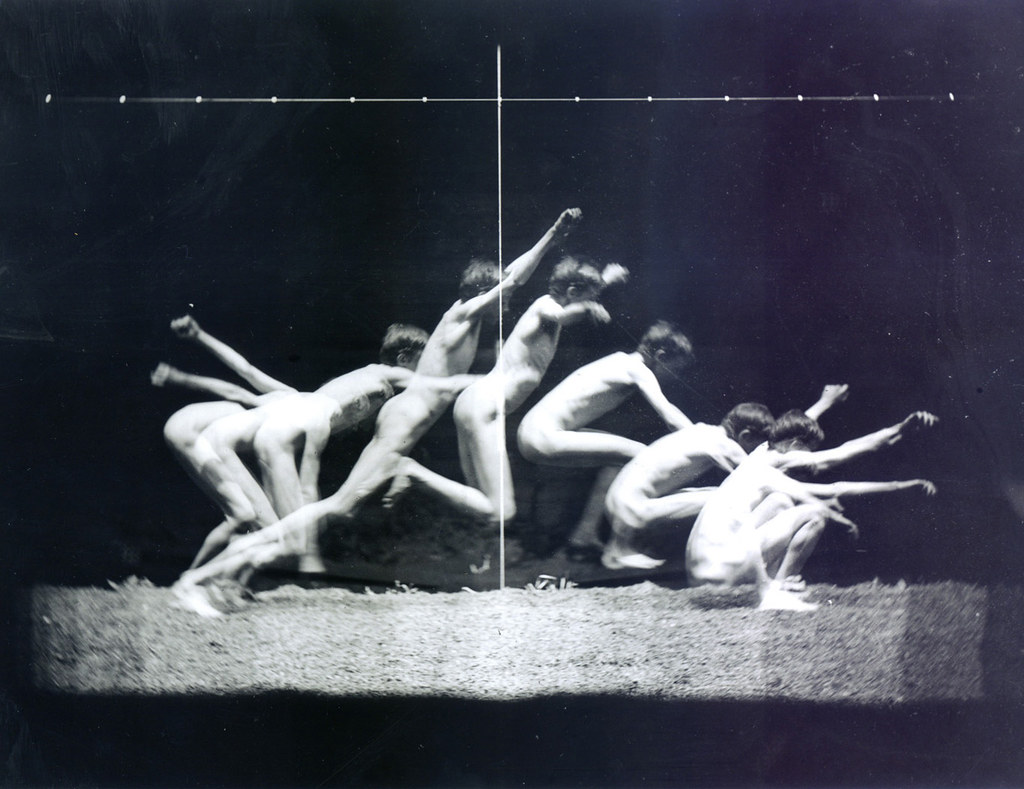
\includegraphics{medias/corpus/muybridge/3695958436_43ae8a57db_b.jpg}
\caption{Chronophotographie ``Eadweard Muybridge'' by floorvan is licensed with CC BY-SA 2.0. To view a copy of this license, visit \url{https://creativecommons.org/licenses/by-sa/2.0/}}
\end{figure}

\begin{itemize}
\tightlist
\item
  \url{https://fr.wikipedia.org/wiki/Ph\%C3\%A9nakistiscope}
\item
  \url{https://fr.wikipedia.org/wiki/Eadweard_Muybridge}
\item
  \url{http://www.artwiki.fr/?EdwardMuybridge}
\end{itemize}

\hypertarget{georges-muxe9lies}{%
\section{Georges Mélies}\label{georges-muxe9lies}}

\begin{figure}
\centering
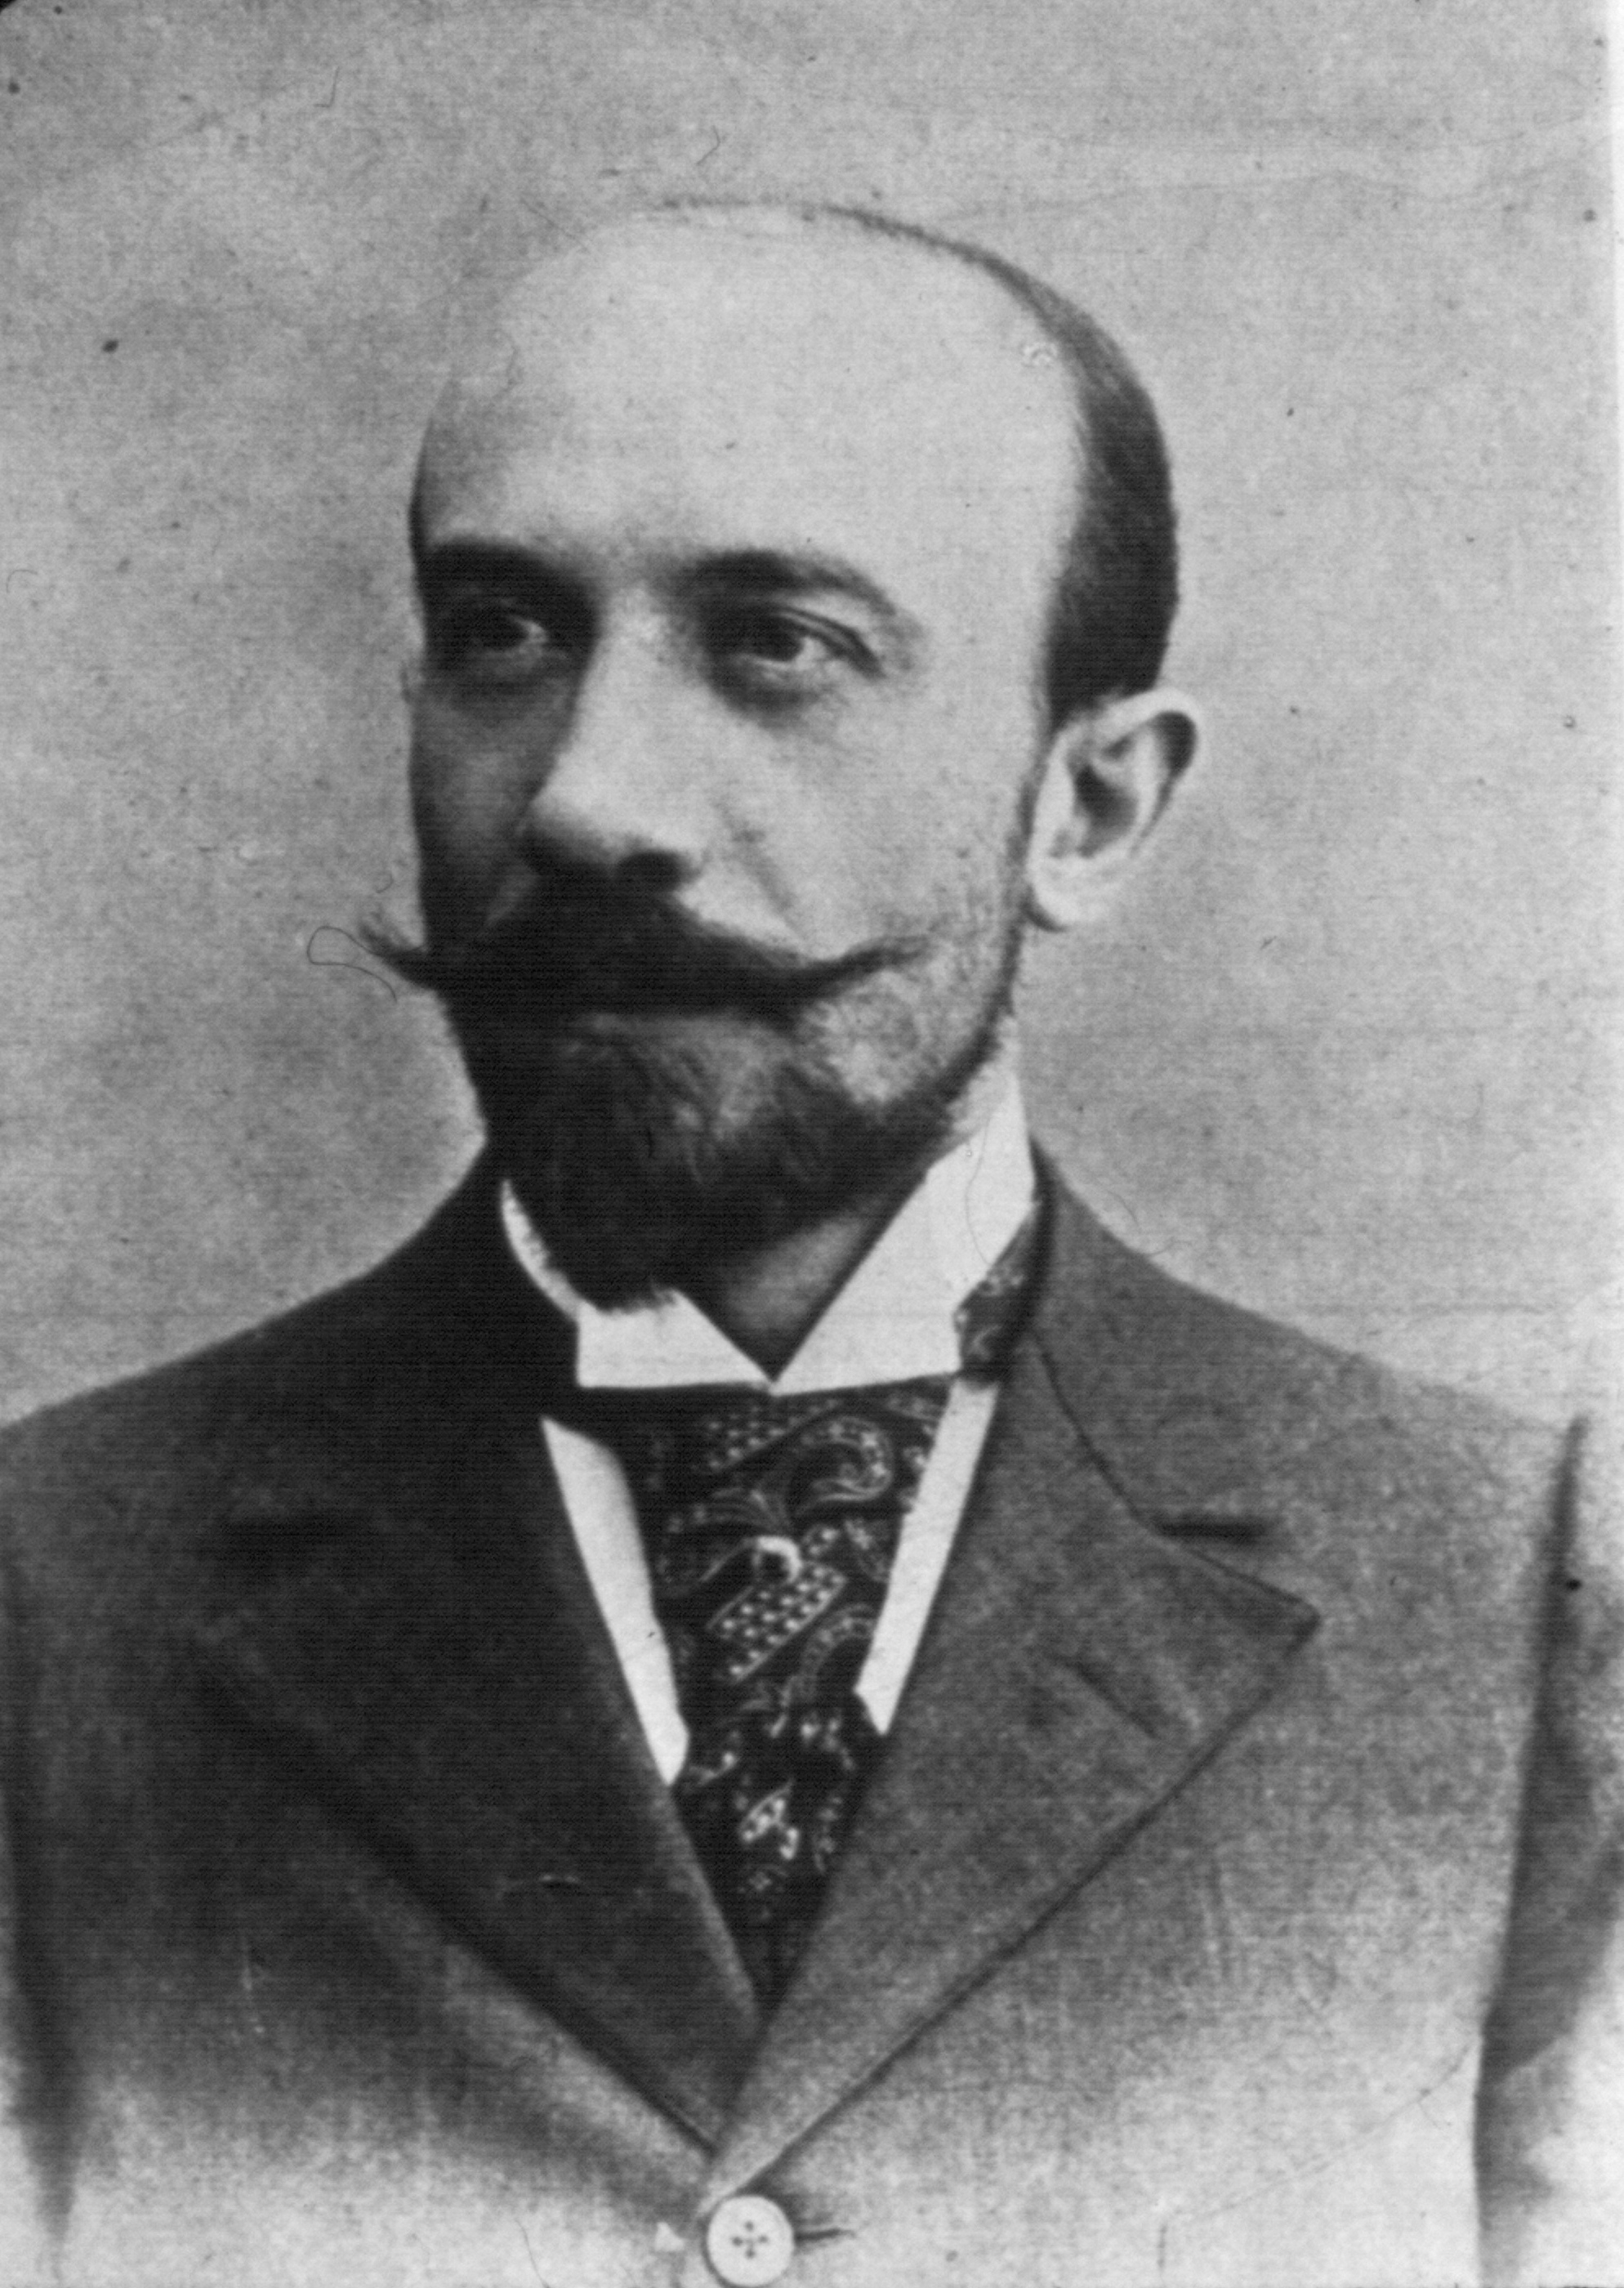
\includegraphics[width=0.5\textwidth,height=\textheight]{medias/corpus/melies/George_Melies.jpg}
\caption{Georges Mélies, 1861-1938}
\end{figure}

\begin{figure}
\centering
\includegraphics[width=0.5\textwidth,height=\textheight]{medias/corpus/melies/voyage_dans_la_lune.gif}
\caption{Le Voyage dans la Lune, 1902}
\end{figure}

\begin{figure}
\centering
\includegraphics[width=0.5\textwidth,height=\textheight]{medias/corpus/melies/sirene_1904.gif}
\caption{La Sirène, 1904}
\end{figure}

\begin{figure}
\centering
\includegraphics[width=0.5\textwidth,height=\textheight]{medias/corpus/melies/b25.gif}
\caption{coloration manuel}
\end{figure}

\begin{itemize}
\tightlist
\item
  \url{http://www.artwiki.fr/?GeorgesMelies}
\item
  \url{https://fr.wikipedia.org/wiki/Georges_M\%C3\%A9li\%C3\%A8s}
\end{itemize}

\hypertarget{dziga-vertov}{%
\section{Dziga Vertov}\label{dziga-vertov}}

\begin{figure}
\centering
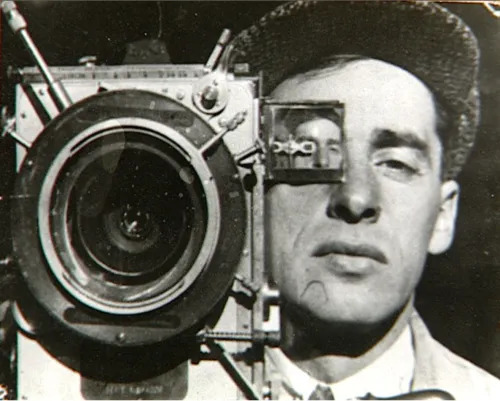
\includegraphics{medias/corpus/vertov/Dziga-Vertov.jpg}
\caption{Dziga Vertov, 1896-1954}
\end{figure}

\begin{figure}
\centering
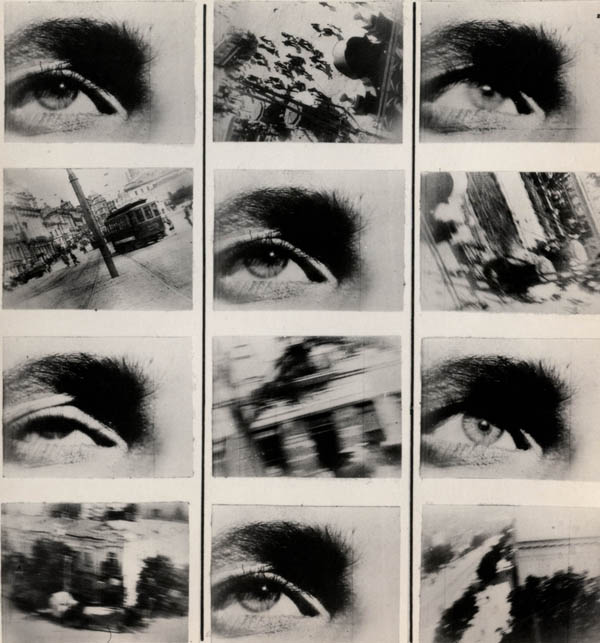
\includegraphics{medias/corpus/vertov/ManWAMovieCamera_1929_DzigaVertov.jpg}
\caption{The Man with the Movie Camera. 1929}
\end{figure}

\begin{figure}
\centering
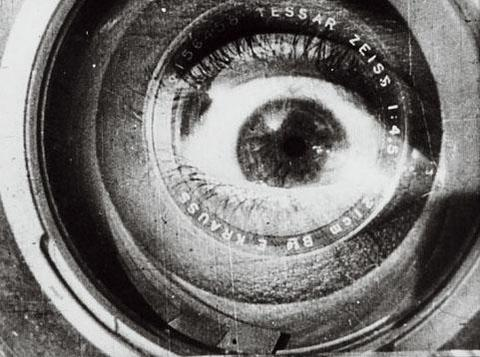
\includegraphics{medias/corpus/vertov/bild.jpg}
\caption{\url{http://www.medienkunstnetz.de/works/der-mann-mit-derkamera/}}
\end{figure}

\begin{itemize}
\tightlist
\item
  \url{https://www.moma.org/explore/inside_out/2010/04/20/dziga-vertov/}
\item
  \url{http://www.artwiki.fr/?DzigaVertov}
\end{itemize}

\hypertarget{futurisme-et-lart-viduxe9o}{%
\section{Futurisme et l'art vidéo}\label{futurisme-et-lart-viduxe9o}}

\hypertarget{umberto-boccioni}{%
\section{Umberto Boccioni}\label{umberto-boccioni}}

\begin{figure}
\centering
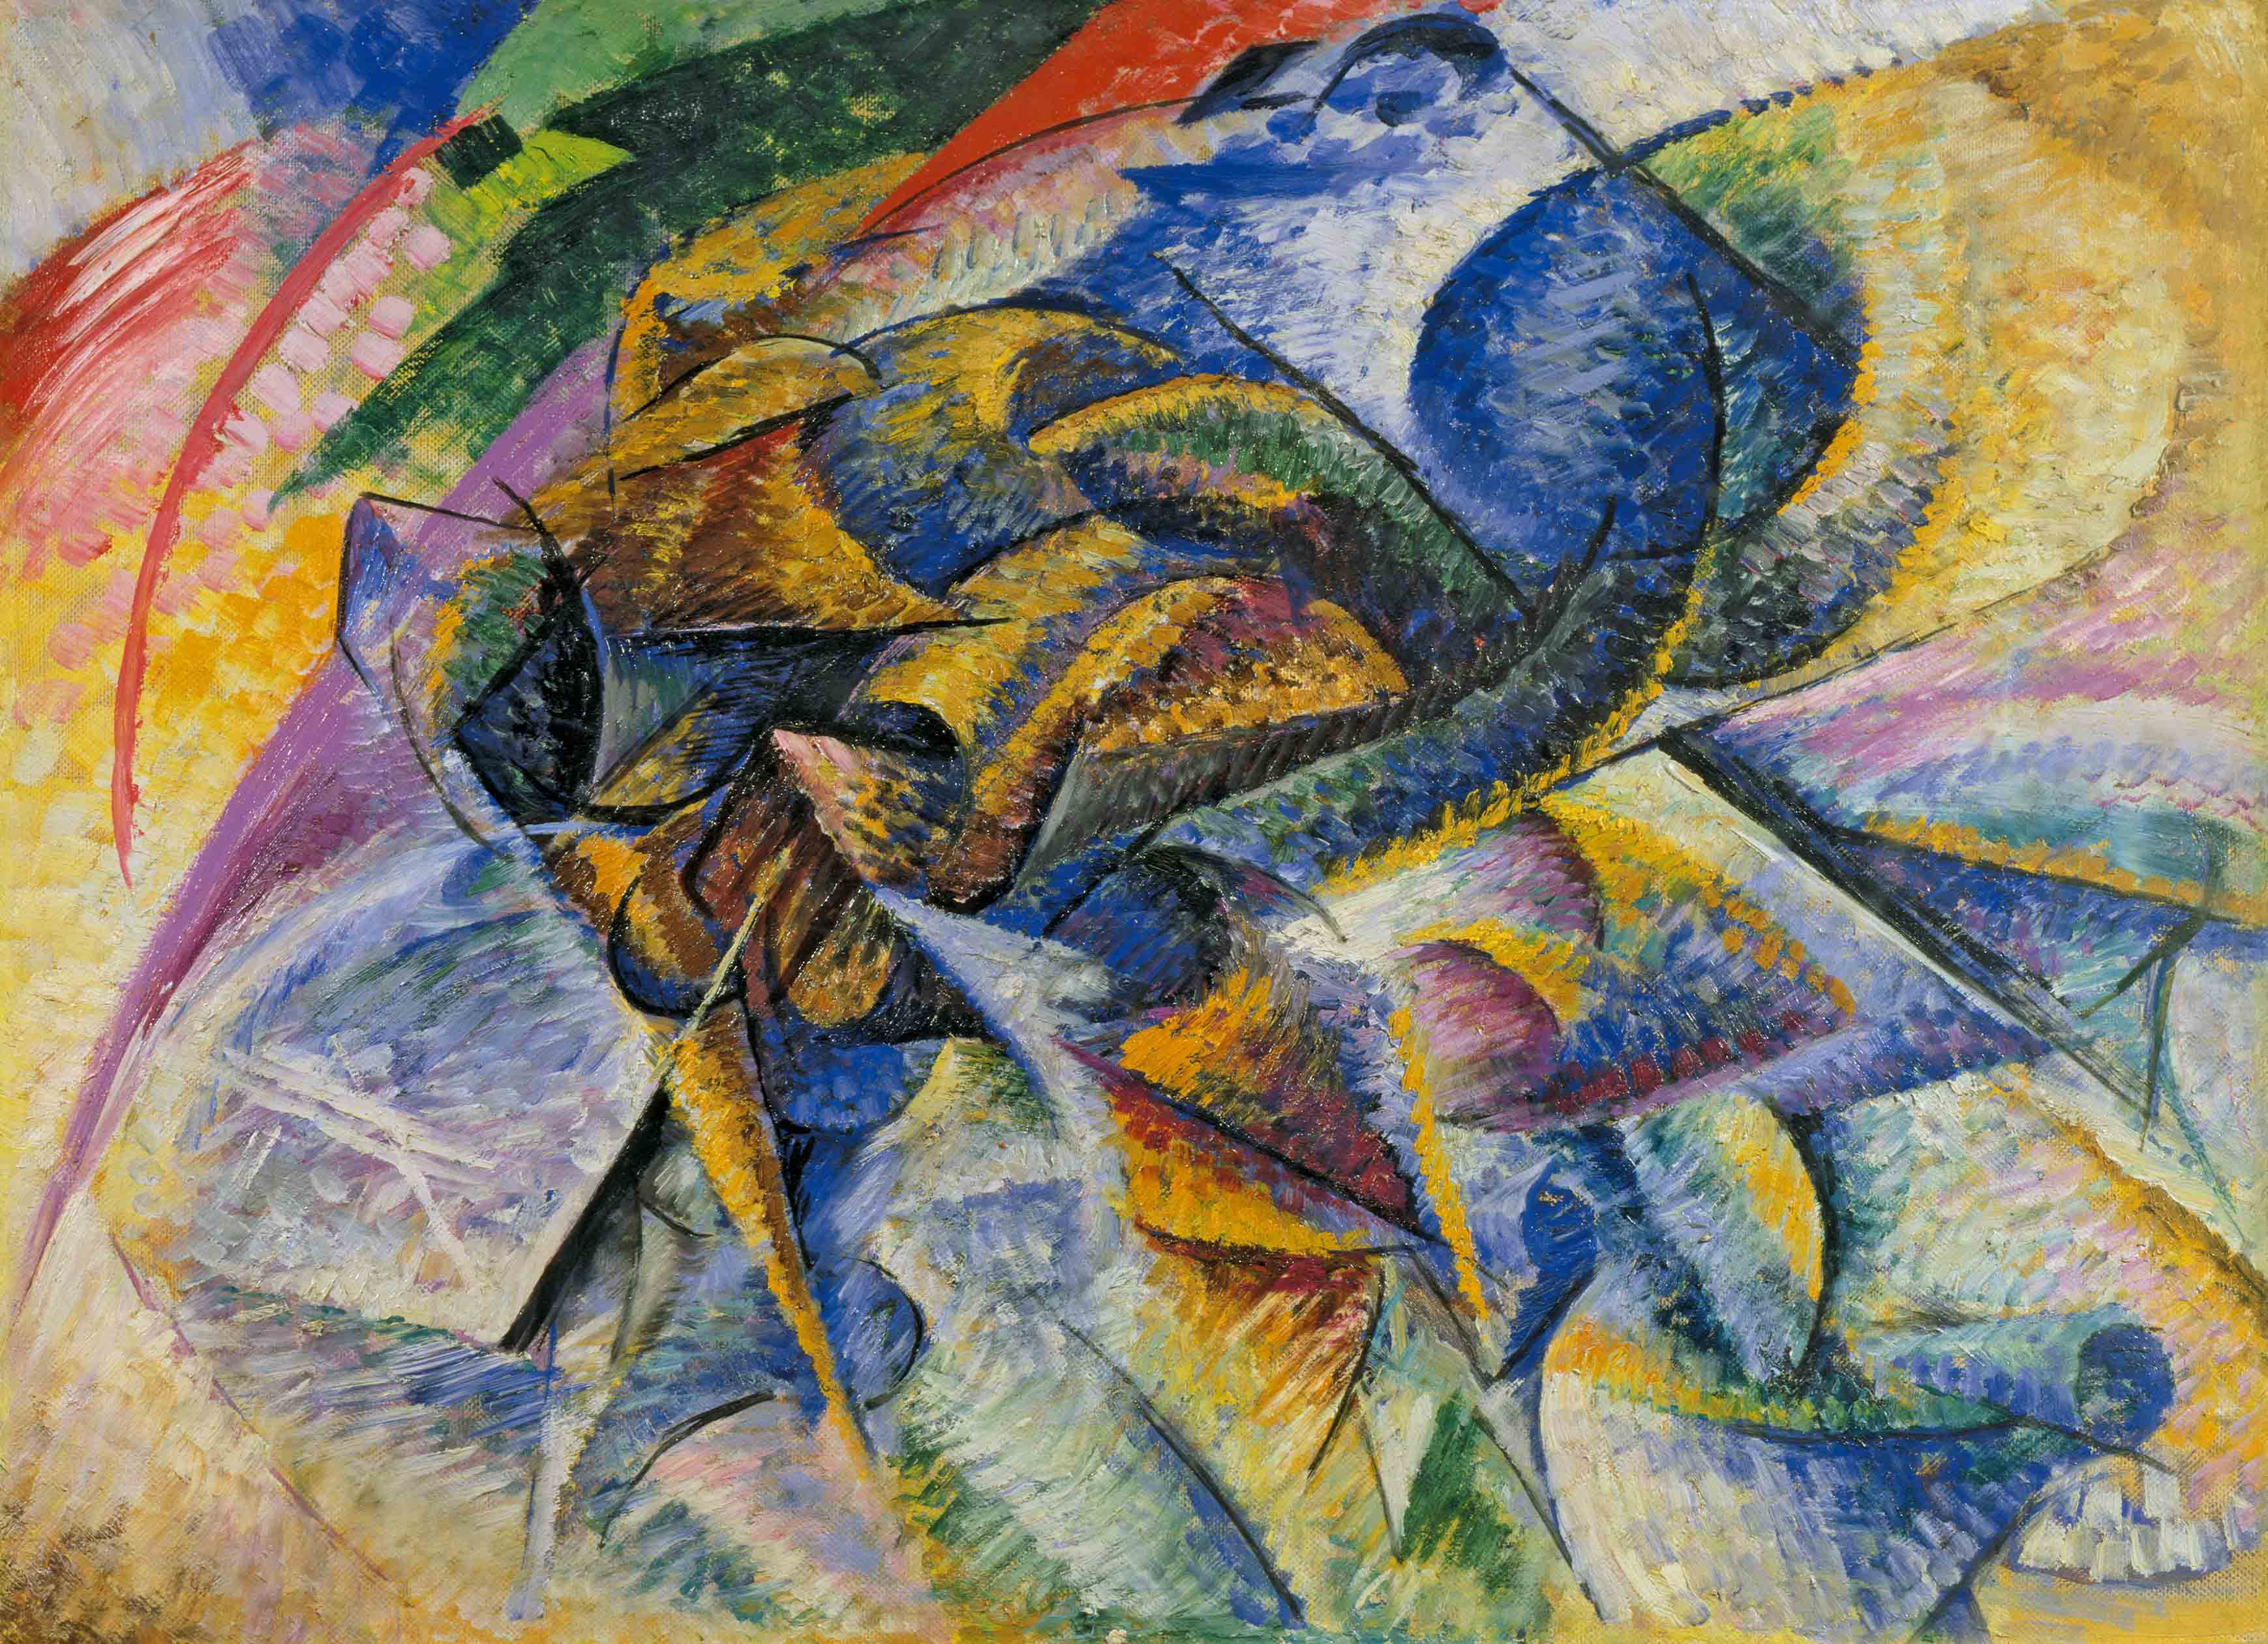
\includegraphics{medias/corpus/boccioni/Umberto_Boccioni,_1913,_Dynamism_of_a_Cyclist_(Dinamismo_di_un_ciclista),_oil_on_canvas,_70_x_95_cm,_Gianni_Mattioli_Collection,_on_long-term_loan_to_the_Peggy_Guggenheim_Collection,_Venice.jpg}
\caption{Par Umberto Boccioni --- Peggy Guggenheim Collection, Domaine public, \url{https://commons.wikimedia.org/w/index.php?curid=38418936}}
\end{figure}

\hypertarget{anton-giulio-bragaglia}{%
\section{Anton Giulio Bragaglia}\label{anton-giulio-bragaglia}}

\begin{figure}
\centering
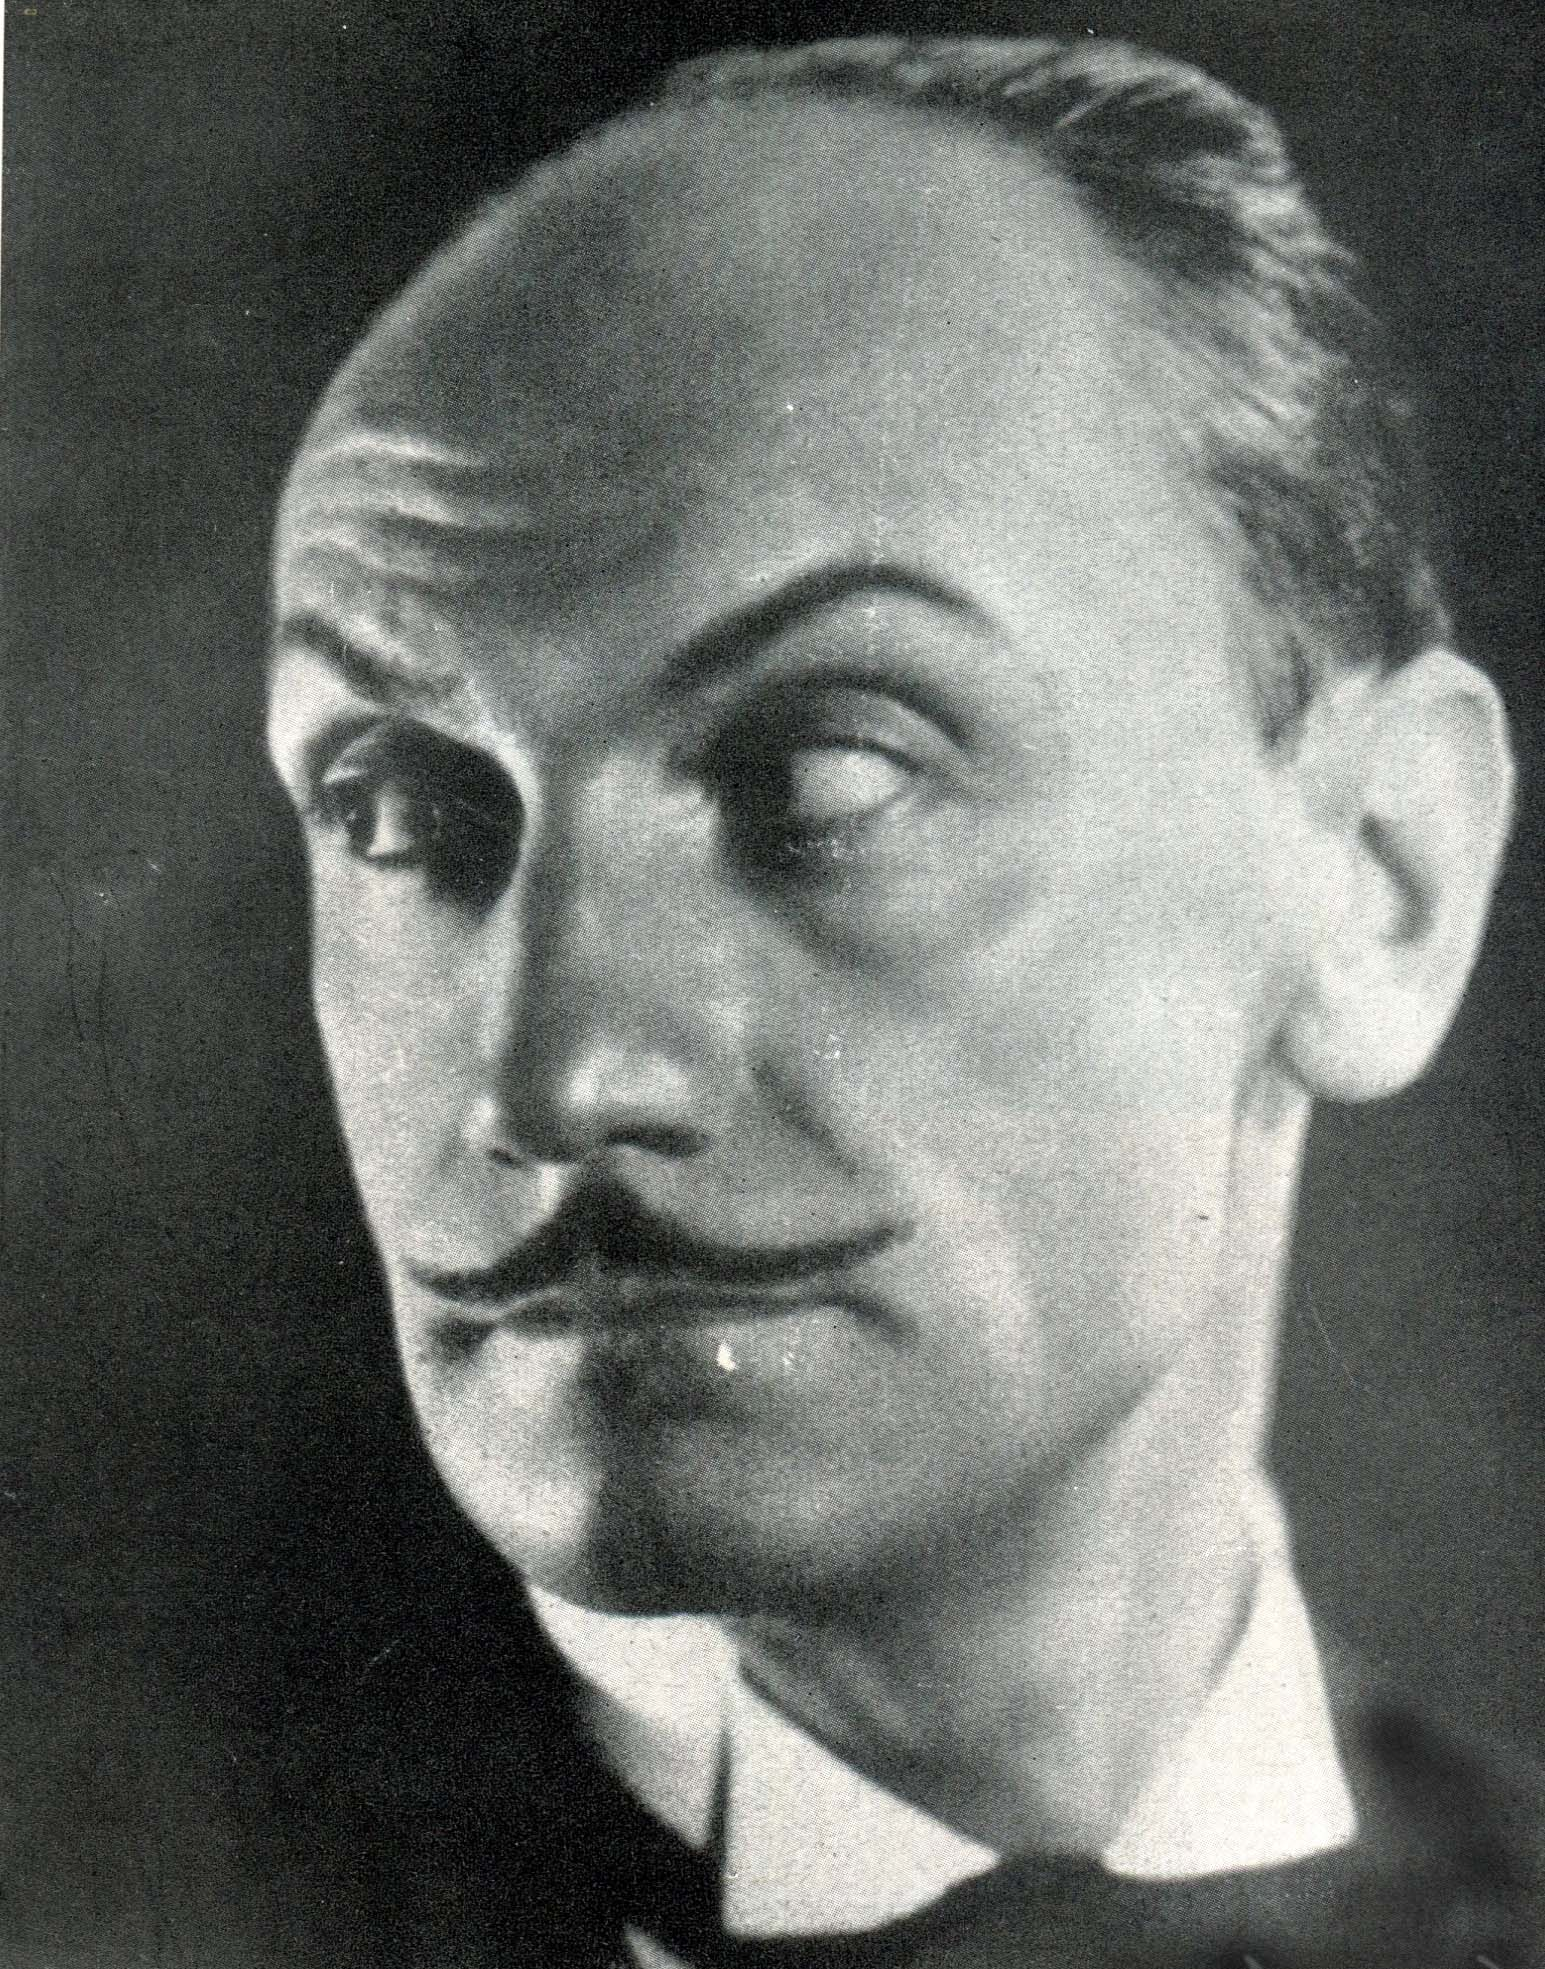
\includegraphics[width=0.5\textwidth,height=\textheight]{medias/corpus/bragaglia/Bragaglia_a_giulio.jpg}
\caption{Anton Giulio Bragaglia, 1890-1960}
\end{figure}

\begin{figure}
\centering
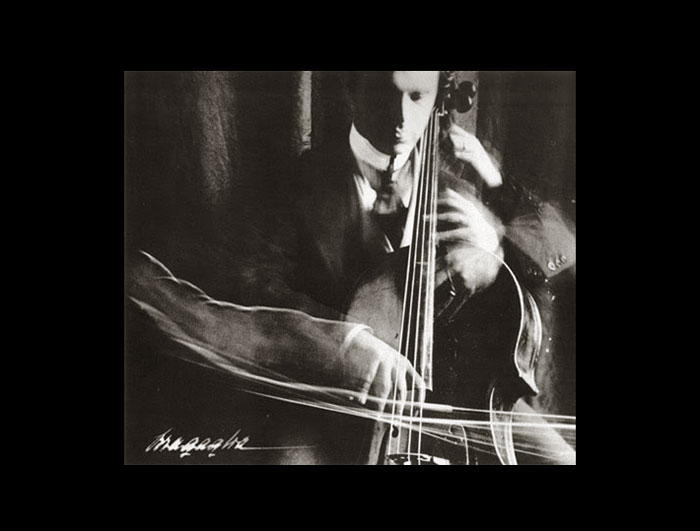
\includegraphics[width=0.75\textwidth,height=\textheight]{medias/corpus/bragaglia/Anton-Giulio-Bragaglia-fotodinamica-02.jpg}
\caption{``Man playing the double bass'', 1911}
\end{figure}

\begin{figure}
\centering
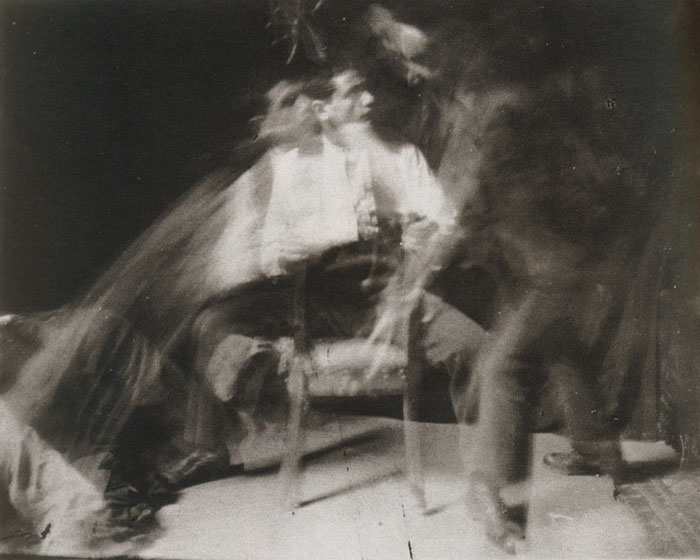
\includegraphics[width=0.75\textwidth,height=\textheight]{medias/corpus/bragaglia/Anton-Giulio-Bragaglia-fotodinamica-04.jpg}
\caption{``The slap'', 1910}
\end{figure}

\begin{figure}
\centering
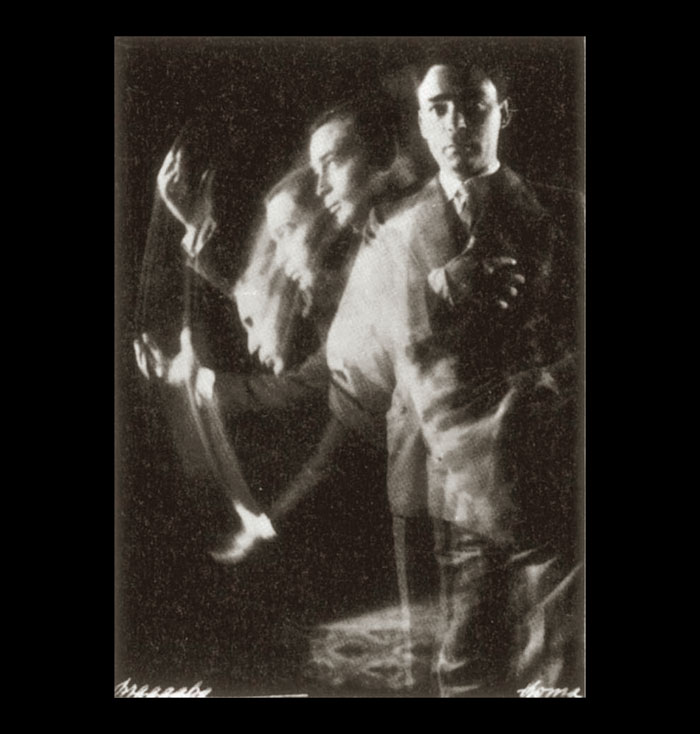
\includegraphics[width=0.75\textwidth,height=\textheight]{medias/corpus/bragaglia/Anton-Giulio-Bragaglia-fotodinamica-05.jpg}
\caption{``Bow'', 1911}
\end{figure}

\begin{figure}
\centering
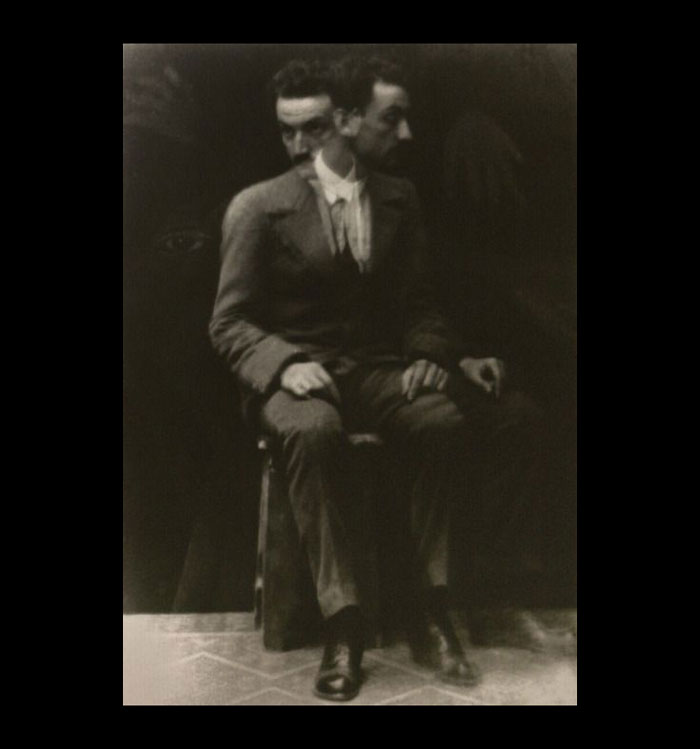
\includegraphics[width=0.75\textwidth,height=\textheight]{medias/corpus/bragaglia/Anton-Giulio-Bragaglia-fotodinamica-06.jpg}
\caption{``Self portrait'', 1913}
\end{figure}

\begin{figure}
\centering
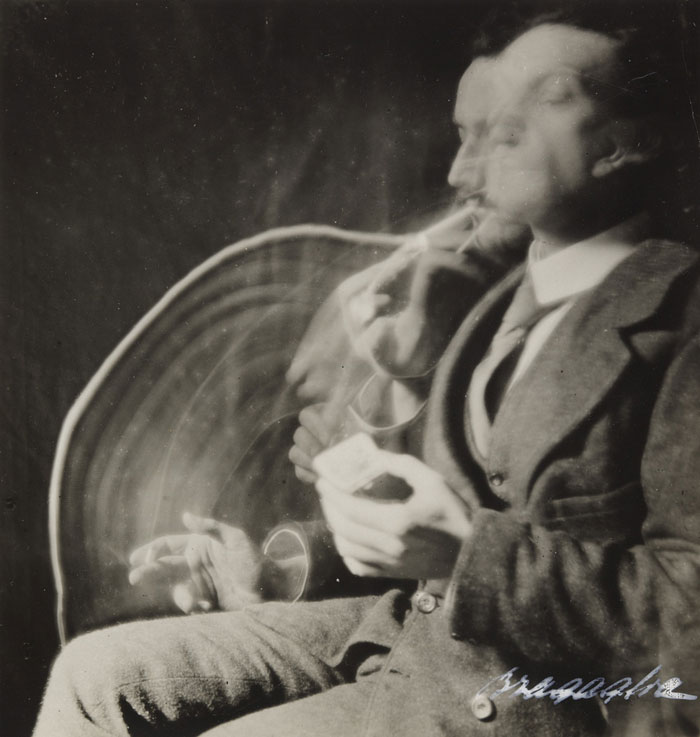
\includegraphics[width=0.75\textwidth,height=\textheight]{medias/corpus/bragaglia/Anton-Giulio-Bragaglia-fotodinamica-07.jpg}
\caption{``Smoker'', 1913}
\end{figure}

\begin{figure}
\centering
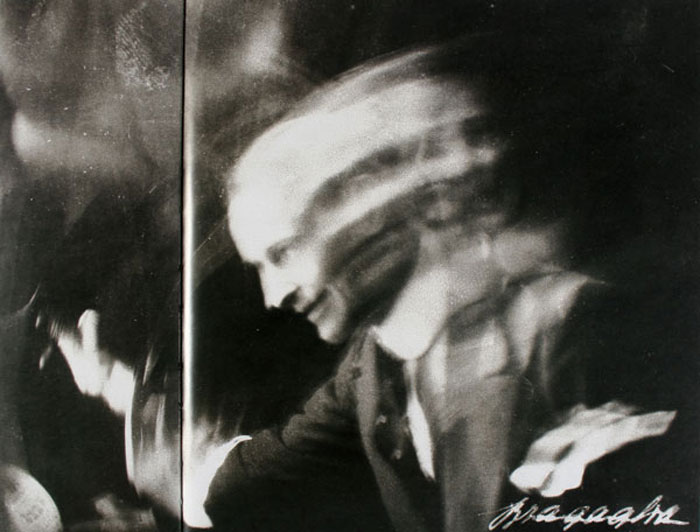
\includegraphics[width=0.75\textwidth,height=\textheight]{medias/corpus/bragaglia/Anton-Giulio-Bragaglia-fotodinamica-08.jpg}
\caption{``Waving'', 1911}
\end{figure}

\begin{figure}
\centering
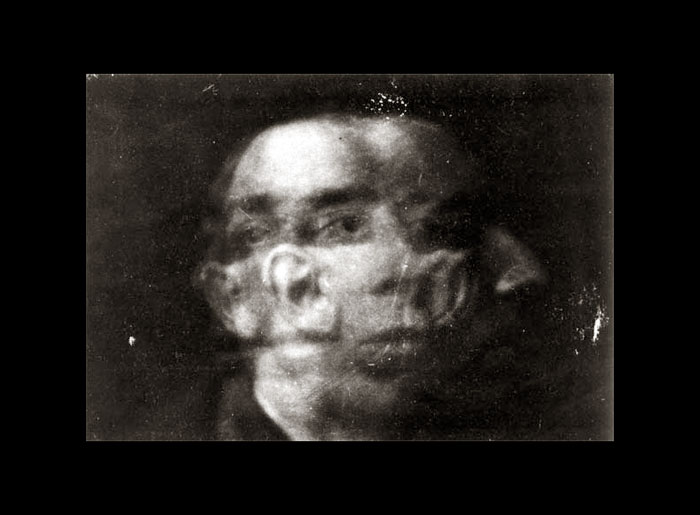
\includegraphics[width=0.75\textwidth,height=\textheight]{medias/corpus/bragaglia/Anton-Giulio-Bragaglia-fotodinamica-09.jpg}
\caption{``Poly-physiognomic portrait of U. Boccioni'', 1913}
\end{figure}

\begin{figure}
\centering
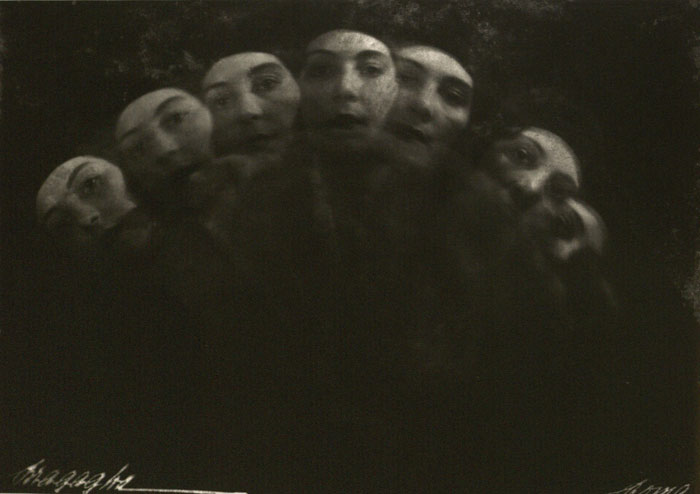
\includegraphics[width=0.75\textwidth,height=\textheight]{medias/corpus/bragaglia/Anton-Giulio-Bragaglia-fotodinamica-11.jpg}
\caption{``Photodynamic portrait of a woman'', 1924}
\end{figure}

\begin{figure}
\centering
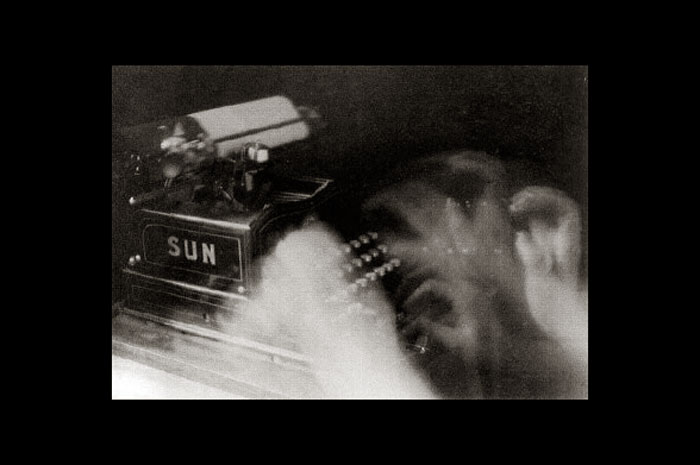
\includegraphics[width=0.75\textwidth,height=\textheight]{medias/corpus/bragaglia/Anton-Giulio-Bragaglia-fotodinamica-12.jpg}
\caption{``Typist'', 1911}
\end{figure}

\begin{figure}
\centering
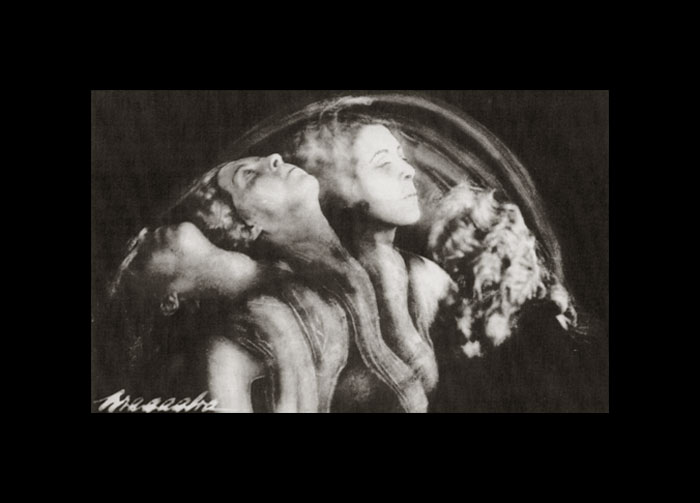
\includegraphics[width=0.75\textwidth,height=\textheight]{medias/corpus/bragaglia/Anton-Giulio-Bragaglia-fotodinamica-13.jpg}
\caption{``L'éventail'', 1928}
\end{figure}

\begin{itemize}
\tightlist
\item
  \url{https://www.italianways.com/past-and-futurism-in-bragaglias-photodynamics/}
\item
  \url{http://www.artwiki.fr/?FuturismeArtvideo}
\end{itemize}

\hypertarget{marcel-duchamp}{%
\section{Marcel Duchamp}\label{marcel-duchamp}}

\begin{figure}
\centering
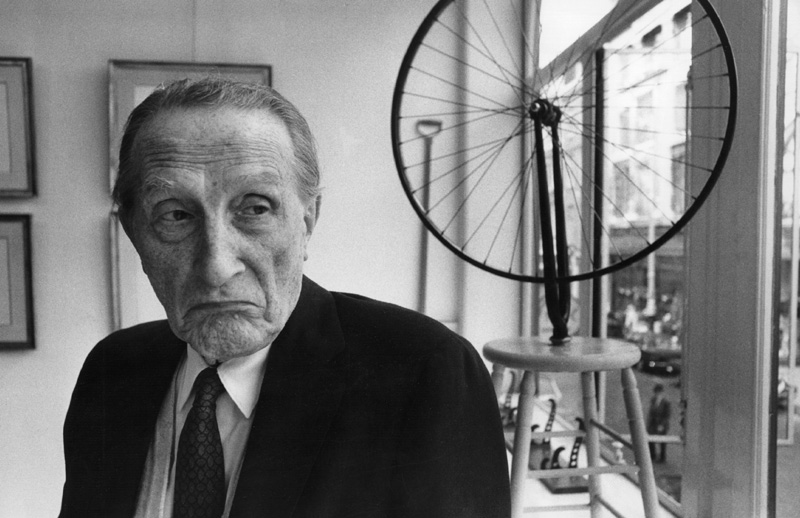
\includegraphics[width=0.75\textwidth,height=\textheight]{medias/corpus/duchamp/MarcelduchampEcologie_portrait_duchamp_20140916163736_20140916163758.jpg}
\caption{Marcel Duchamp, 1887-1968}
\end{figure}

\begin{figure}
\centering
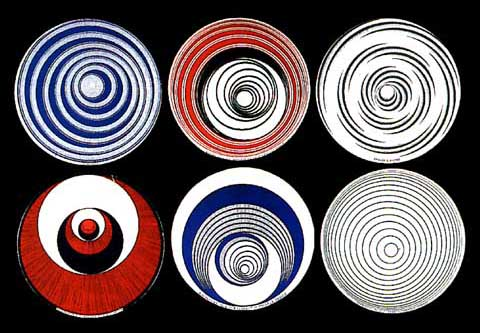
\includegraphics{medias/corpus/duchamp/MarcelduchampEcologie_duchamp_rotoreliefs_1935_20140917095658_20140917095757.jpg}
\caption{Rotoreliefs, 1926}
\end{figure}

\begin{figure}
\centering
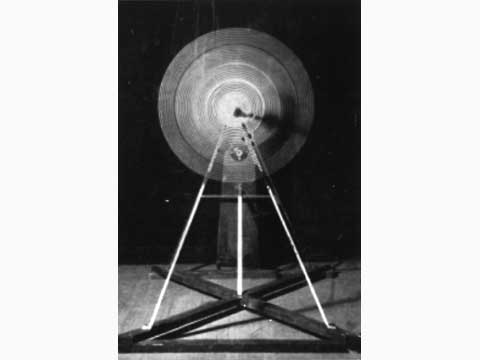
\includegraphics{medias/corpus/duchamp/MarcelduchampEcologie_ducha_rotative_plaque_verre_20140917224650_20140917225046.jpg}
\caption{Plaque rotative sur verre, \textasciitilde1920-1923}
\end{figure}

\begin{quote}
Rotoreliefs, 1926
\end{quote}

\begin{quote}
La participation du spectateur, l'oeuvre ouverte:

«Ce sont les regardeurs qui font les tableaux»

«Somme toute, l'artiste n'est pas seul à accomplir l'acte de création car le spectateur établit le contact de l'oeuvre avec le monde extérieur en déchiffrant et en interprétant ses qualifications profondes et par là, ajoute sa propre contribution au processus créatif.»\\
-- Marcel Duchamp
\end{quote}

\begin{quote}
Il invente par ses Rotoreliefs l'Art cinétique
\end{quote}

\begin{itemize}
\tightlist
\item
  \url{http://www.artwiki.fr/?MarcelduchampEcologie}
\item
  \url{https://fr.wikipedia.org/wiki/Marcel_Duchamp}
\end{itemize}

\hypertarget{stan-brakhage}{%
\section{Stan Brakhage}\label{stan-brakhage}}

\begin{figure}
\centering
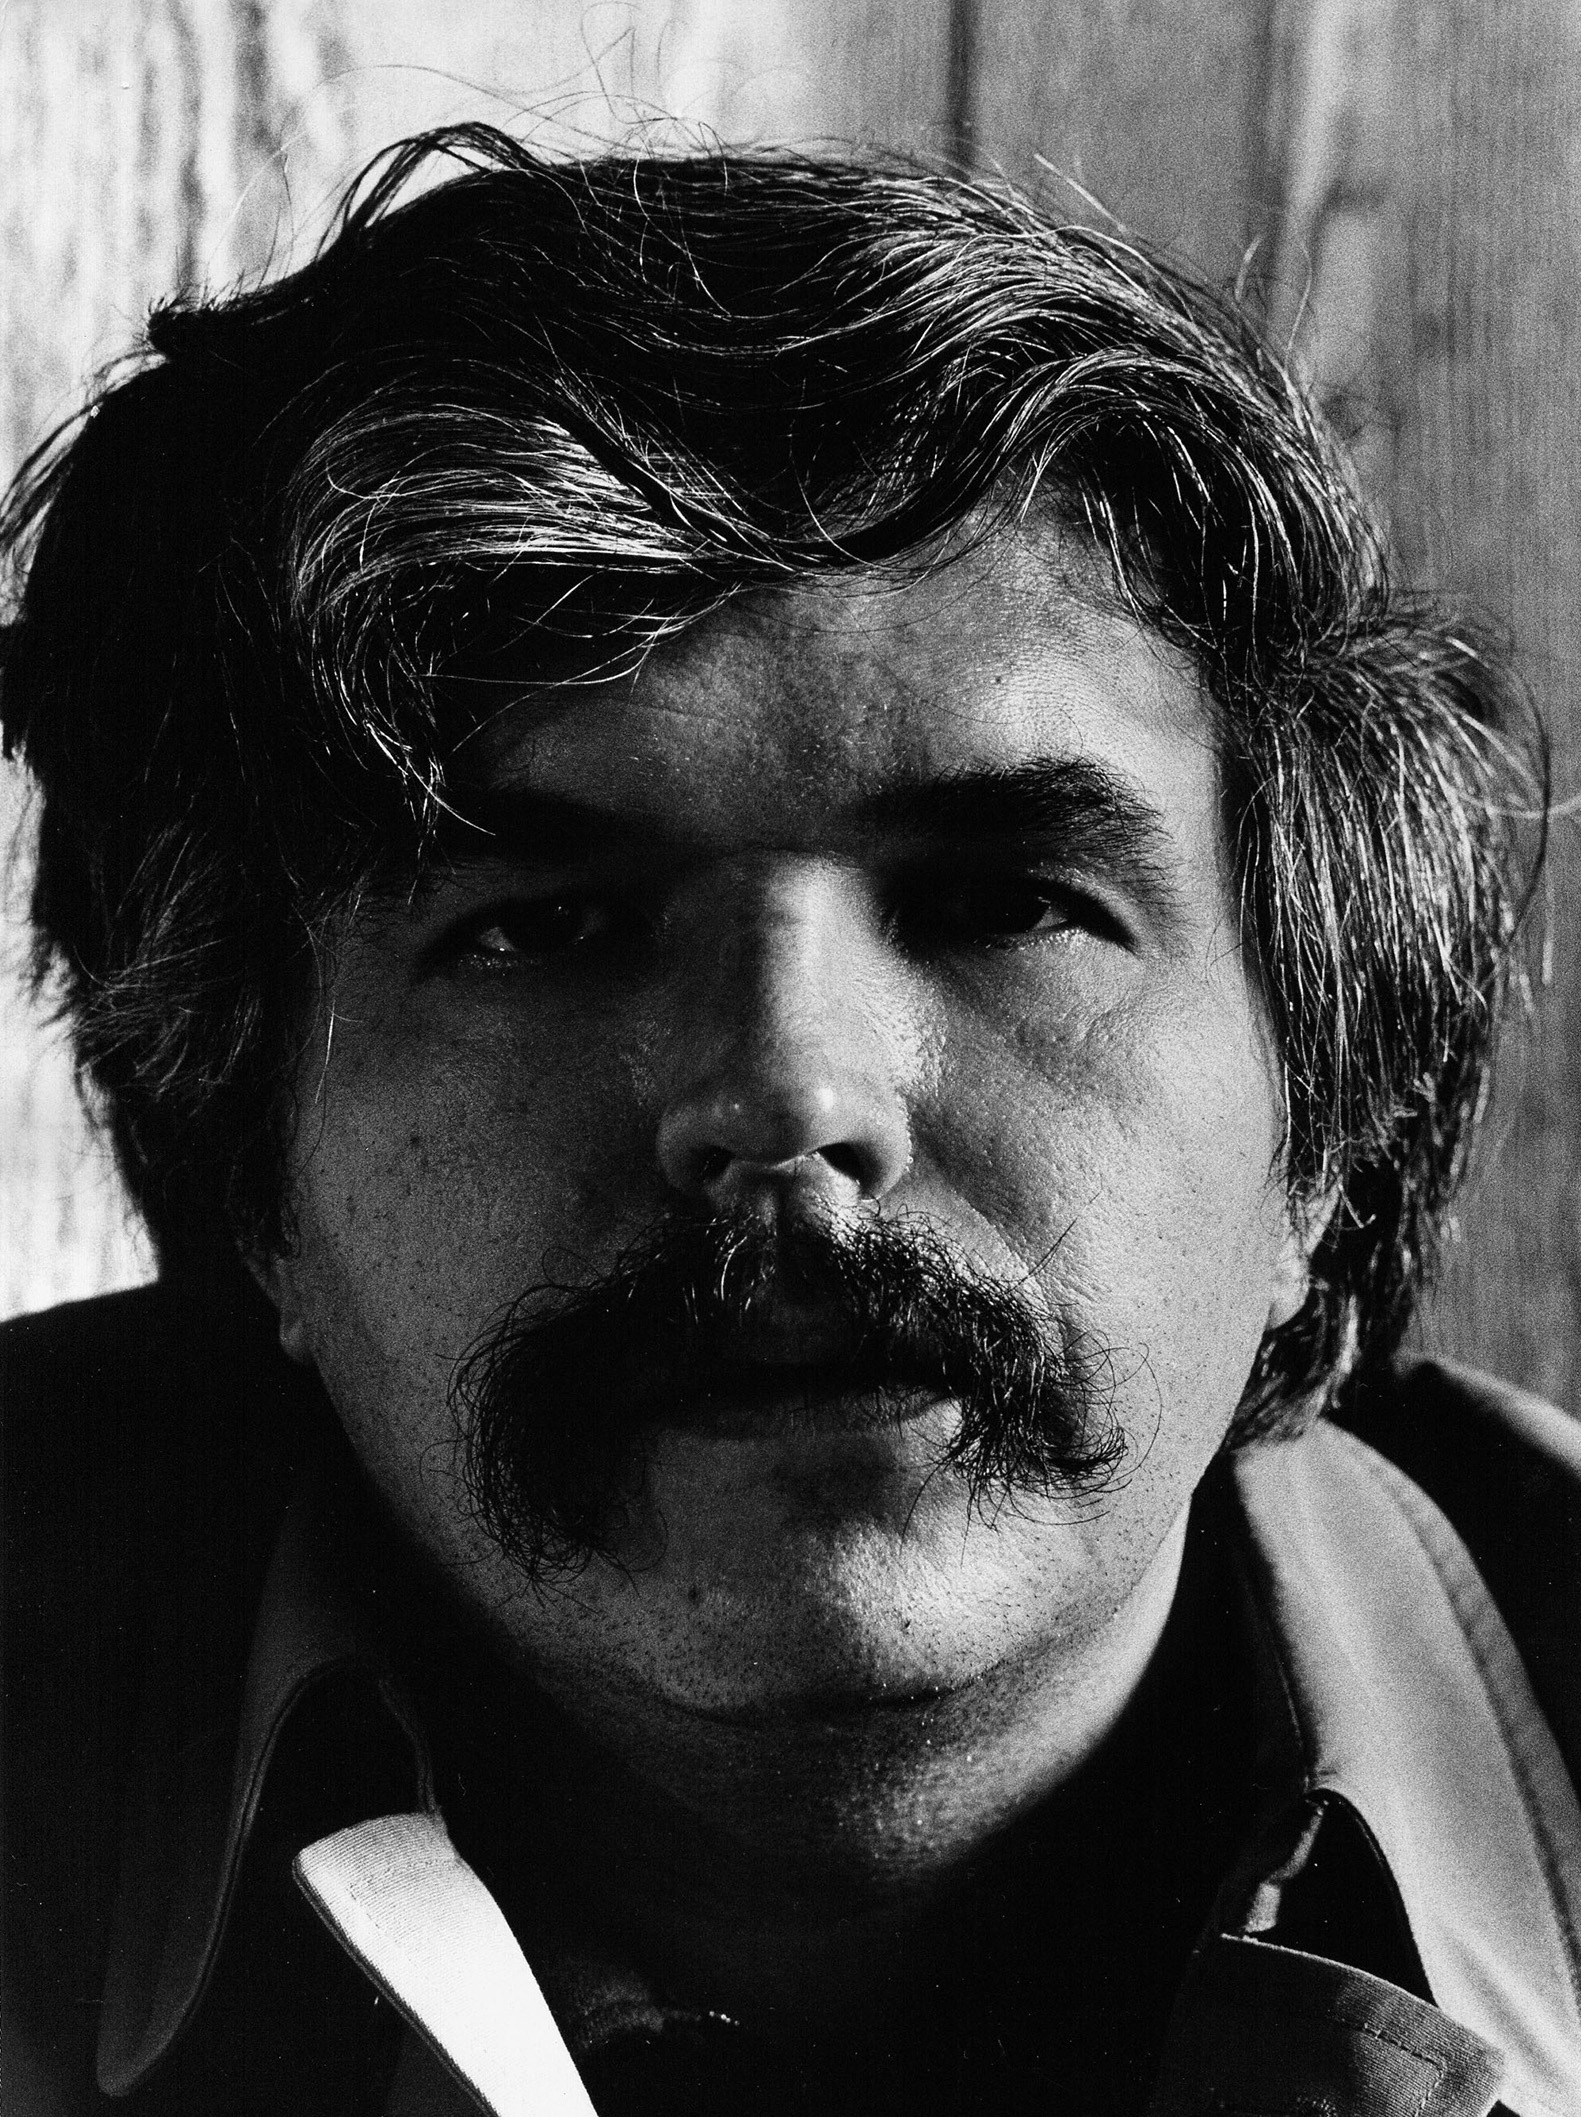
\includegraphics[width=0.5\textwidth,height=\textheight]{medias/corpus/brakhage/Stan_Brakhage_(circa_1976).jpg}
\caption{Stan Brakhage, 1933-2003}
\end{figure}

\begin{quote}
Mothlight - Stan Brakhage {[}1963{]}

On retrouve cette technique d'intervention sur la pellicule de manière encore plus marquée pour Mothlight, en 1963. Pour ce court-métrage, Brakhage ne s'est pas servi de caméra : il a inséré entre deux pellicules des feuilles et des insectes, ce qui donne de nouveau un rythme de défilement extrêmement rapide.
art wiki
\end{quote}

\begin{quote}
The Dante Quartet - Stan Brakhage {[}1987{]}
\end{quote}

\begin{itemize}
\tightlist
\item
  \url{http://www.artwiki.fr/?StanBrakhage}
\item
  \url{https://en.wikipedia.org/wiki/Stan_Brakhage}
\end{itemize}

\hypertarget{john-milton-cage}{%
\section{John Milton Cage}\label{john-milton-cage}}

\begin{itemize}
\tightlist
\item
  \url{http://www.artwiki.fr/?JohnCage}
\end{itemize}

\hypertarget{norman-mclaren}{%
\section{Norman McLaren}\label{norman-mclaren}}

\begin{figure}
\centering
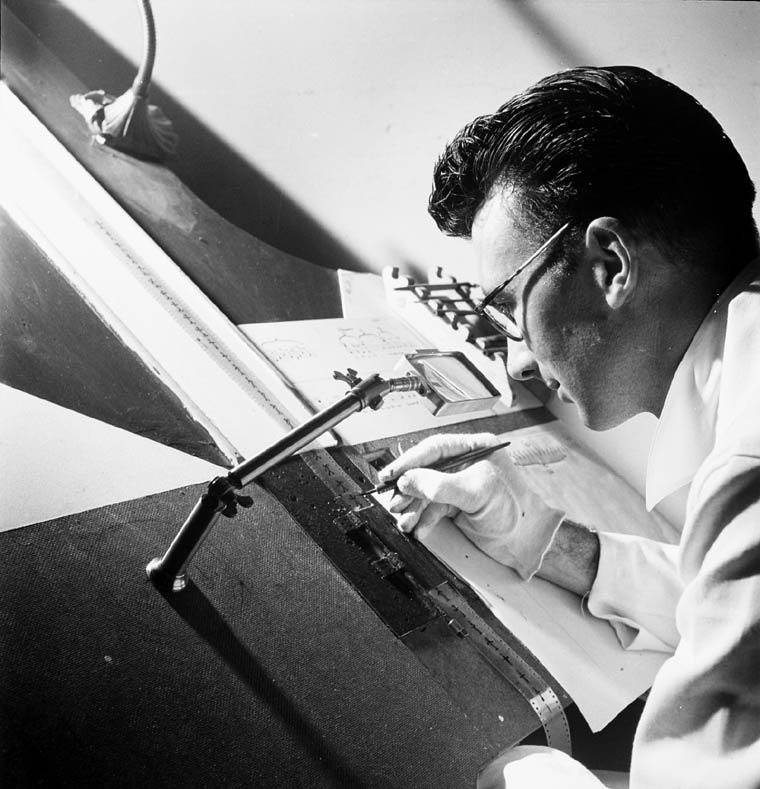
\includegraphics{medias/corpus/mclaren/Norman_McLaren_drawing_on_film_-_1944.jpg}
\caption{Norman McLaren, 1914-1987}
\end{figure}

\begin{quote}
Pen Point Percussion (1958)
\end{quote}

\begin{quote}
Mosaic (1965)
\end{quote}

\begin{quote}
Synchromy (1971)
\end{quote}

\begin{quote}
A Phantasy in Colors (1949)
\end{quote}

\begin{itemize}
\tightlist
\item
  \url{https://www.onf.ca/cineastes/norman-mclaren/}
\item
  \url{https://fr.wikipedia.org/wiki/Norman_McLaren}
\item
  \url{http://www.artwiki.fr/?NormanMcLaren}
\end{itemize}

\hypertarget{et-le-duxe9but-de-la-viduxe9o}{%
\section{1960 et le début de la vidéo}\label{et-le-duxe9but-de-la-viduxe9o}}

\begin{figure}

{\centering 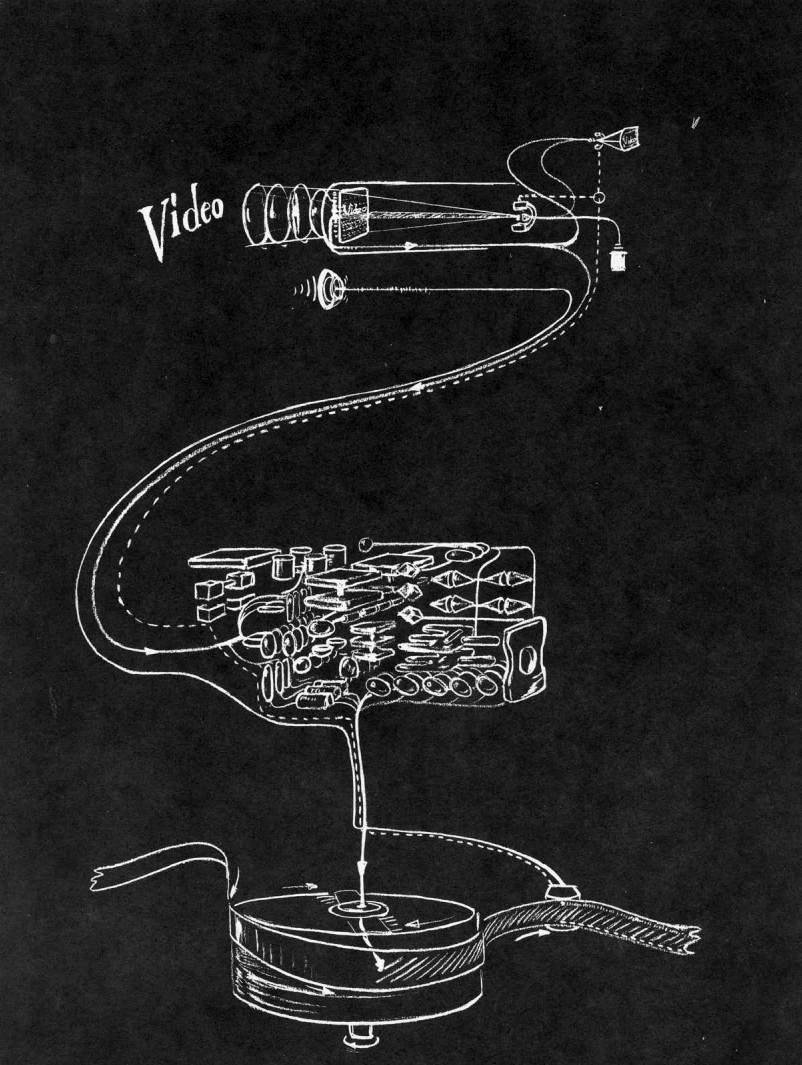
\includegraphics[width=0.49\linewidth]{medias/corpus/1960/Charles_Bensinger_video_guide_2} 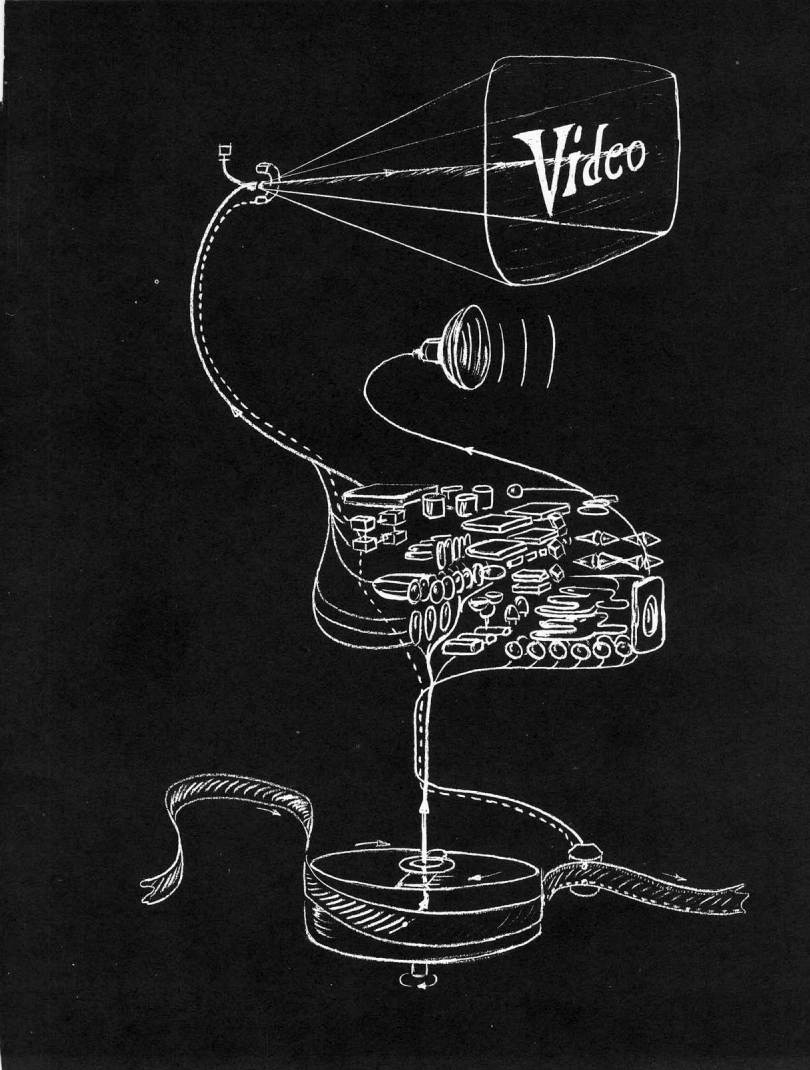
\includegraphics[width=0.49\linewidth]{medias/corpus/1960/Charles_Bensinger_video_guide_3} 

}

\caption{Enregistrer et reproduire depuis un support magnétique}\label{fig:unnamed-chunk-2}
\end{figure}

\begin{itemize}
\tightlist
\item
  \url{https://cool.culturalheritage.org/videopreservation/vid_guide/}
\item
  \url{https://en.wikipedia.org/wiki/Portapak}
\end{itemize}

\hypertarget{nam-june-paik}{%
\section{Nam June Paik}\label{nam-june-paik}}

\begin{figure}
\centering
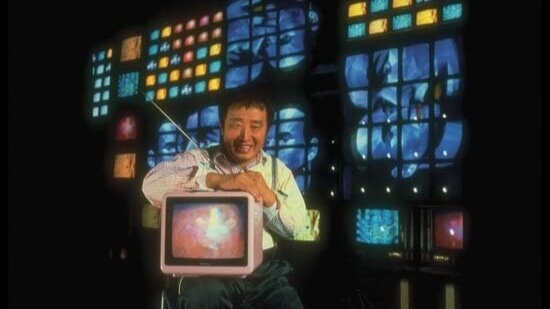
\includegraphics{medias/corpus/paik/paik_10.jpg}
\caption{Nam June Paik, 1932-2006}
\end{figure}

\begin{figure}

{\centering 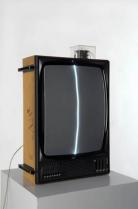
\includegraphics[width=0.32\linewidth]{medias/corpus/paik/____NamJunepaik_0220452w_namjunepaikzenfortv1961975_vignette_300_209_20150414152312_20150414153250} 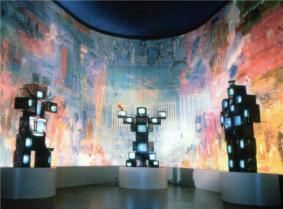
\includegraphics[width=0.32\linewidth]{medias/corpus/paik/__NamJunepaik_22222_vignette_300_209_20150414121039_20150414121316} 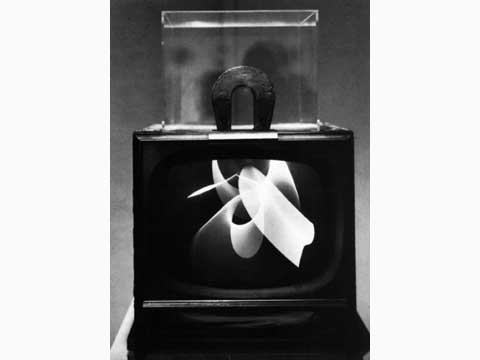
\includegraphics[width=0.32\linewidth]{medias/corpus/paik/_NamJunepaik_paik_magnet_tv_20150506194428_20150506194457} 

}

\caption{Enregistrer et reproduire depuis un support magnétique}\label{fig:unnamed-chunk-3}
\end{figure}

\begin{itemize}
\tightlist
\item
  \url{http://www.artwiki.fr/?NamjunePaik}
\item
  \url{https://fr.wikipedia.org/wiki/Nam_June_Paik}
\end{itemize}

\hypertarget{steina-and-woody-vasulka}{%
\section{Steina and Woody Vasulka}\label{steina-and-woody-vasulka}}

\begin{itemize}
\tightlist
\item
  \url{https://www.fondation-langlois.org/html/f/page.php?NumPage=435}
\item
  \url{http://www.sonore-visuel.fr/fr/evenement/au-commencement-etait-le-bruit-la-poesie-electronique-de-steina-et-woody-vasulka}
\item
  \url{http://www.vasulka.org/}
\item
  \url{https://www.fondation-langlois.org/html/f/page.php?NumPage=495}
\item
  \url{https://www.eai.org/artists/steina-and-woody-vasulka/biography}
\end{itemize}

\hypertarget{wolf-vostell}{%
\section{Wolf Vostell}\label{wolf-vostell}}

\begin{itemize}
\tightlist
\item
  \url{http://www.artwiki.fr/?WolfVostell}
\end{itemize}

\hypertarget{les-levine}{%
\section{Les Levine}\label{les-levine}}

\begin{itemize}
\tightlist
\item
  \url{http://www.artwiki.fr/?LesLevine}
\end{itemize}

\hypertarget{section}{%
\section{1970}\label{section}}

\hypertarget{valie-export}{%
\section{Valie Export}\label{valie-export}}

\begin{itemize}
\tightlist
\item
  \url{http://www.artwiki.fr/?ValieExport}
\end{itemize}

\hypertarget{frank-gillette}{%
\section{Frank Gillette}\label{frank-gillette}}

\begin{itemize}
\tightlist
\item
  \url{http://www.artwiki.fr/?FrankGillette}
\end{itemize}

\hypertarget{michael-snow}{%
\section{Michael Snow}\label{michael-snow}}

\begin{itemize}
\tightlist
\item
  \url{http://www.artwiki.fr/?MichaelSnow}
\end{itemize}

\hypertarget{jud-yalkut}{%
\section{Jud Yalkut}\label{jud-yalkut}}

\begin{itemize}
\tightlist
\item
  \url{http://www.artwiki.fr/?JudYalkut}
\end{itemize}

\hypertarget{shigeko-kubota}{%
\section{Shigeko Kubota}\label{shigeko-kubota}}

\begin{itemize}
\tightlist
\item
  \url{http://www.artwiki.fr/?ShigekoKubota}
\end{itemize}

\hypertarget{marina-abramovic-ulay}{%
\section{Marina Abramovic \& Ulay}\label{marina-abramovic-ulay}}

\begin{itemize}
\tightlist
\item
  \url{http://www.artwiki.fr/?AbramoviculayVideo70}
\end{itemize}

\hypertarget{jean-pierre-boyer}{%
\section{Jean-Pierre Boyer}\label{jean-pierre-boyer}}

\begin{figure}
\centering
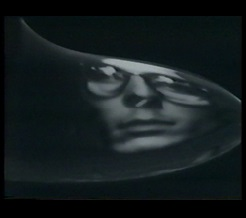
\includegraphics[width=0.5\textwidth,height=\textheight]{medias/corpus/boyer/Portrait-e2288.jpg}
\caption{Jean-Pierre Boyer, 1950 -}
\end{figure}

\begin{figure}
\centering
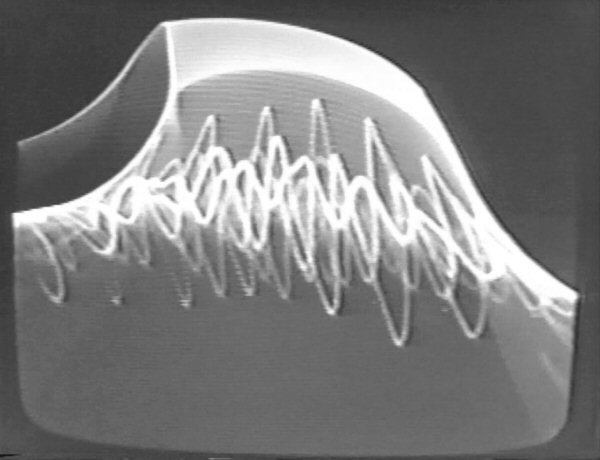
\includegraphics{medias/corpus/boyer/Chant-magnetique.jpg}
\caption{Chant magnetique}
\end{figure}

\begin{figure}
\centering
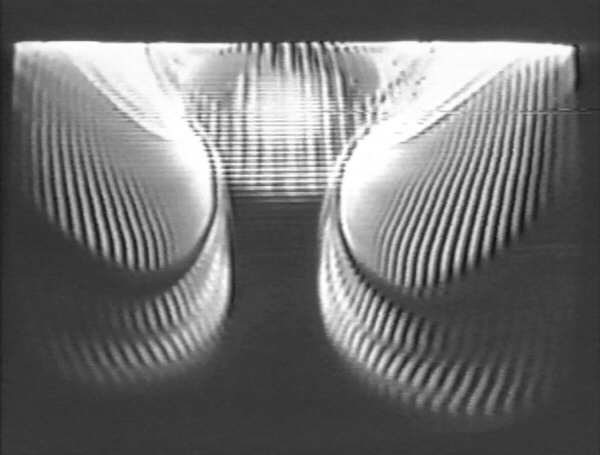
\includegraphics{medias/corpus/boyer/Eau.jpg}
\caption{Eau}
\end{figure}

\begin{figure}
\centering
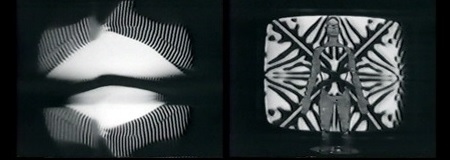
\includegraphics{medias/corpus/boyer/L-Amertube-2f5ae.jpg}
\caption{Amertube}
\end{figure}

\begin{figure}
\centering
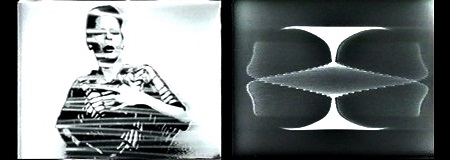
\includegraphics{medias/corpus/boyer/Phonoptic-33bd2.jpg}
\caption{Phonoptic}
\end{figure}

\begin{figure}
\centering
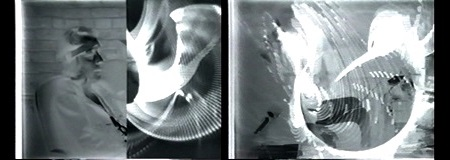
\includegraphics{medias/corpus/boyer/Video-Cortex-b8d37.jpg}
\caption{video cortex}
\end{figure}

\begin{itemize}
\tightlist
\item
  \url{https://www.horschamp.qc.ca/spip.php?article535}
\item
  \url{https://vitheque.com/en/directors/jean-pierre-boyer}
\item
  \url{https://www.fondation-langlois.org/html/e/page.php?NumPage=1839}
\item
  \url{https://www.fondation-langlois.org/html/e/research.php?zoom=3\&Filtres=5\&Numero=i00005710\&MotsCles=Jean-Pierre+Boyer}
\end{itemize}

\hypertarget{david-rokeby}{%
\section{David Rokeby}\label{david-rokeby}}

\begin{figure}
\centering
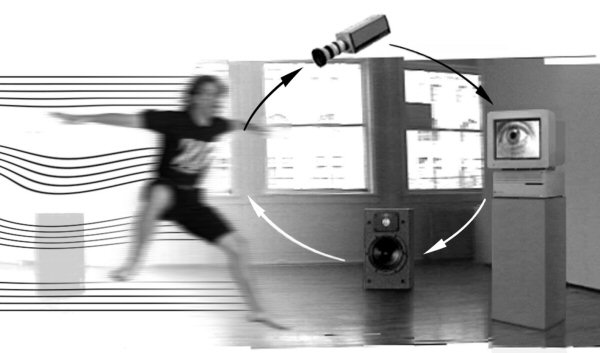
\includegraphics[width=0.75\textwidth,height=\textheight]{medias/corpus/rokeby/d00004229-wide.jpg}
\caption{David Rokeby, 1960-}
\end{figure}

Very Nervous System (1986-90)

Very Nervous System (1987 version) from David Rokeby on Vimeo.

Very Nervous System (1982-1991) by David Rokeby from David Rokeby on Vimeo.

\begin{itemize}
\tightlist
\item
  \url{https://www.fondation-langlois.org/html/e/page.php?NumPage=1951}
\item
  \url{http://www.davidrokeby.com/vns.html}
\item
  \url{https://www.arshake.com/en/interview-david-rokeby/}
\end{itemize}

\hypertarget{ryoji-ikeda}{%
\section{Ryoji Ikeda}\label{ryoji-ikeda}}

\url{https://www.ryojiikeda.com/}

\url{http://www.artwiki.fr/?RyojiIkeda}

\hypertarget{contemporains}{%
\section{Contemporains}\label{contemporains}}

\hypertarget{alexandre-burton-julien-roy}{%
\section{Alexandre Burton + Julien Roy}\label{alexandre-burton-julien-roy}}

trois pièces avec des titres - MUTEK Montréal 2017 from artificiel on Vimeo.

\begin{itemize}
\tightlist
\item
  \url{https://www.artificiel.org/projet/3pieces}
\end{itemize}

\hypertarget{sabrina-rattuxe9}{%
\section{Sabrina Ratté}\label{sabrina-rattuxe9}}

\begin{itemize}
\tightlist
\item
  \url{http://sabrinaratte.com/FLORALIA-2021}
\item
  \url{https://infrarouge.org/productions\#/introduction-la-violence/}
\item
  \url{http://sabrinaratte.com/filter/VIDEOS}
\item
  \url{https://ellephant.org/artists/sabrina-ratte/}
\end{itemize}

\hypertarget{allison-moore}{%
\section{Allison Moore}\label{allison-moore}}

\begin{itemize}
\tightlist
\item
  \url{http://www.allisonmoore.net/about}
\end{itemize}

\hypertarget{guillaume-valluxe9e}{%
\section{Guillaume Vallée}\label{guillaume-valluxe9e}}

\begin{itemize}
\tightlist
\item
  \url{https://www.gvallee.com/}
\end{itemize}

\hypertarget{tind-thisisnotdesign}{%
\section{TIND :: thisisnotdesign}\label{tind-thisisnotdesign}}

\begin{itemize}
\tightlist
\item
  \url{http://tind.org/}
\end{itemize}

\hypertarget{duxe9rapages}{%
\section{Dérapages}\label{duxe9rapages}}

\hypertarget{deadline-17-avril-2021-date-limite-pour-soumettre-un-film.}{%
\subsection{DEADLINE 17 avril 2021 : date limite pour soumettre un film.}\label{deadline-17-avril-2021-date-limite-pour-soumettre-un-film.}}

\url{https://derapage.ca/?fbclid=IwAR1VeYPaM7V9x1IoA0_eM9vtRQpD9VERCpwDl4oRTxOXK_n41Vol67EQH5E}

\hypertarget{duxe9rapages-1}{%
\subsection{Dérapages}\label{duxe9rapages-1}}

\url{https://www.youtube.com/results?search_query=derapage+festival}

\hypertarget{festivals}{%
\section{Festivals}\label{festivals}}

\hypertarget{file-electronic-language-international-festival}{%
\subsection{\texorpdfstring{\emph{FILE} Electronic Language International Festival}{FILE Electronic Language International Festival}}\label{file-electronic-language-international-festival}}

\begin{itemize}
\tightlist
\item
  \url{https://file.org.br/videoarte_2018/}
\item
  \url{https://file.org.br/file_sp_2019/}
\item
  \url{https://file.org.br/videoarte_2019/}
\end{itemize}

\hypertarget{mutek}{%
\subsection{Mutek}\label{mutek}}

\begin{itemize}
\tightlist
\item
  \url{https://mutek.org/en/artists/}
\end{itemize}

\hypertarget{isea-inter-society-for-the-electronic-arts}{%
\subsection{\texorpdfstring{\emph{ISEA} Inter-Society for the Electronic Arts}{ISEA Inter-Society for the Electronic Arts}}\label{isea-inter-society-for-the-electronic-arts}}

\begin{itemize}
\tightlist
\item
  \url{https://art2020.isea-international.org/art-portfolio/}
\item
  \url{https://isea2020.isea-international.org/wp-content/uploads/2020/10/ISEA-Programme-book-271020.pdf}
\end{itemize}

\hypertarget{htmlles-ada-x}{%
\subsection{HTMlles (Ada X)}\label{htmlles-ada-x}}

\begin{itemize}
\tightlist
\item
  \url{https://www.ada-x.org/productions/festival/}
\end{itemize}

\hypertarget{historique}{%
\chapter{Historique du traitement vidéo}\label{historique}}

\hypertarget{evolution_historique_technologies}{%
\section{Évolution des technologies associées}\label{evolution_historique_technologies}}

De l'argentique au magnétique, du magnétique au numérique (1960 à aujourd'hui)

\begin{itemize}
\tightlist
\item
  Présentation Synthèse de l'histoire de la vidéo artistique

  \begin{itemize}
  \tightlist
  \item
    \url{http://iasl.uni-muenchen.de/links/GCA\%20IV\%20Video\%20Tools.pdf}
  \end{itemize}
\item
  ligne de temps exaustive de l'art vidéo et de ses acteurs

  \begin{itemize}
  \tightlist
  \item
    \url{http://iasl.uni-muenchen.de/links/GCA-IV.1e.html\#Video}
  \item
    Contient des informations pertinente sur la génèse de la synthèse vidéo
  \end{itemize}
\item
  L'évolution du graphisme assité par ordinateur

  \begin{itemize}
  \tightlist
  \item
    \url{http://iasl.uni-muenchen.de/links/GCA-III.2e.html}
  \end{itemize}
\item
  Exemple de d'utilisation de moteur de jeu et de technique de post-production lors de la production lors du tournage de la série Mandalorian

  \begin{itemize}
  \tightlist
  \item
    \url{https://arstechnica.com/gaming/2020/02/the-mandalorian-was-shot-on-a-holodeck-esque-set-with-unreal-engine-video-shows/}
  \end{itemize}
\end{itemize}

\hypertarget{evolution_historique}{%
\section{Évolution historique du traitement vidéo dans les différentes formes d'art}\label{evolution_historique}}

\begin{itemize}
\tightlist
\item
  \href{https://www.lerecit.fr/wp-content/uploads/2017/08/introduction-\%C3\%A0-lArt-Vid\%C3\%A9o.pdf}{Introduction à l'art vidéo.pdf}

  \begin{itemize}
  \tightlist
  \item
    Contient des définitions et exemples pour :

    \begin{itemize}
    \tightlist
    \item
      Art vidéo
    \item
      performance
    \item
      installation
    \item
      installation interactive
    \end{itemize}
  \end{itemize}
\end{itemize}

\hypertarget{evolution_historique_performance}{%
\subsection{Performance}\label{evolution_historique_performance}}

\begin{itemize}
\tightlist
\item
  \url{http://www.artwiki.fr/?PerformancE}
\item
  \url{https://fr.vikidia.org/wiki/Performance_(art)}
\item
  \url{https://fr.wikipedia.org/wiki/Performance_(art)}
\end{itemize}

\hypertarget{evolution_historique_installation}{%
\subsection{Installation}\label{evolution_historique_installation}}

\begin{itemize}
\tightlist
\item
  \url{https://fr.wikipedia.org/wiki/Installation_(art)}
\item
  \url{https://en.wikipedia.org/wiki/Installation_art}
\end{itemize}

\hypertarget{cinuxe9ma-expuxe9rimental}{%
\subsection{Cinéma Expérimental}\label{cinuxe9ma-expuxe9rimental}}

\begin{itemize}
\tightlist
\item
  \url{http://www.artwiki.fr/?CinemaExperimental}
\end{itemize}

\hypertarget{le-vee-jaying-ou-simplement-vjing}{%
\subsection{\texorpdfstring{Le \textbf{Vee-Jaying} ou simplement \textbf{VJing}*}{Le Vee-Jaying ou simplement VJing*}}\label{le-vee-jaying-ou-simplement-vjing}}

\begin{itemize}
\tightlist
\item
  \url{https://fr.wikipedia.org/wiki/Vid\%C3\%A9o-jockey}
\item
  \url{https://en.wikipedia.org/wiki/VJing}
\item
  \url{http://jhroy.ca/z/machina/syn-jimmy.htm}
\item
  \url{https://en.wikipedia.org/wiki/Music_visualization}
\item
  \url{https://vimeo.com/groups/vjstv}
\item
  \url{https://www.antivj.com/}
\item
  \url{https://cdm.link/tag/vj/}
\end{itemize}

\hypertarget{evolution_historique_language}{%
\section{Langages et moyens expressifs de l'image en mouvement}\label{evolution_historique_language}}

\begin{itemize}
\tightlist
\item
  \url{https://www.fondation-langlois.org/html/f/page.php?NumPage=689}

  \begin{itemize}
  \tightlist
  \item
    Ce qui reste des images du futur : Ancrage sociohistorique de l'art vidéo interactif\\
  \end{itemize}
\item
  \url{https://esse.ca/fr/la-question-de-lart-video}

  \begin{itemize}
  \tightlist
  \item
    Trace la quête existentielle de la vidéo à travers le temps depuis sa génèse.
  \end{itemize}
\end{itemize}

Autre liens

\begin{itemize}
\tightlist
\item
  \url{https://demainlequotidien.up.coop/democratisation-de-la-culture/la-frontiere-entre-theatre-et-cinema-va-t-elle-disparaitre}
\end{itemize}

\hypertarget{lexique}{%
\chapter{Lexique technique et technologique}\label{lexique}}

\hypertarget{lexique_composantes}{%
\section{Constituantes du signal vidéo}\label{lexique_composantes}}

\hypertarget{ruxe9solution}{%
\subsection{Résolution}\label{ruxe9solution}}

Associé au nombre de pixels horizontaux et verticaux composant une image.
Généralement exprimé par le nombre de pixels horizontaux multiplié par le nombre de pixels verticaux

\[
résolution  = PixelsH * PixelsV 
\]

\hypertarget{cadence}{%
\subsection{Cadence}\label{cadence}}

Associé à la vitesse, généralement exprimé en images / secondes

\[
cadence (img/s) = images / secondes
\]

\begin{itemize}
\tightlist
\item
  \href{https://frames-per-second.appspot.com}{Démonstration en ligne de la variation de la cadence}
\end{itemize}

\hypertarget{trame}{%
\subsection{Trame}\label{trame}}

Soit progressive ou entrelacée
* \href{https://web.archive.org/web/20140222010640/http://neuron2.net/LVG/interlacing.html}{Trame (progressif/entrelacé)}

\hypertarget{progressive}{%
\subsubsection{Progressive}\label{progressive}}

\begin{itemize}
\tightlist
\item
  Image complète transmise à chaque rafraichissement
\item
  associée à la lettre \textbf{p}
\end{itemize}

\hypertarget{entrelacuxe9e}{%
\subsubsection{Entrelacée}\label{entrelacuxe9e}}

\begin{itemize}
\tightlist
\item
  Image partielle transmise à chaque rafraichissement
\item
  Généralement alterné entre les champs verticaux pairs et impairs
\item
  Associée à la lettre \textbf{i} pour \emph{interlaced}
\end{itemize}

\hypertarget{nature-du-signal}{%
\section{Nature du signal}\label{nature-du-signal}}

\hypertarget{analogue-vs-numuxe9rique}{%
\subsection{Analogue vs numérique}\label{analogue-vs-numuxe9rique}}

\hypertarget{interpruxe9tation-de-la-fluctuation-uxe9lectrique}{%
\subsubsection{Interprétation de la fluctuation électrique}\label{interpruxe9tation-de-la-fluctuation-uxe9lectrique}}

\hypertarget{analogue-virgule-flottante}{%
\paragraph{Analogue : virgule flottante}\label{analogue-virgule-flottante}}

Toutes les possibilités entre le minimum et le maximum de voltage

\begin{figure}

{\centering 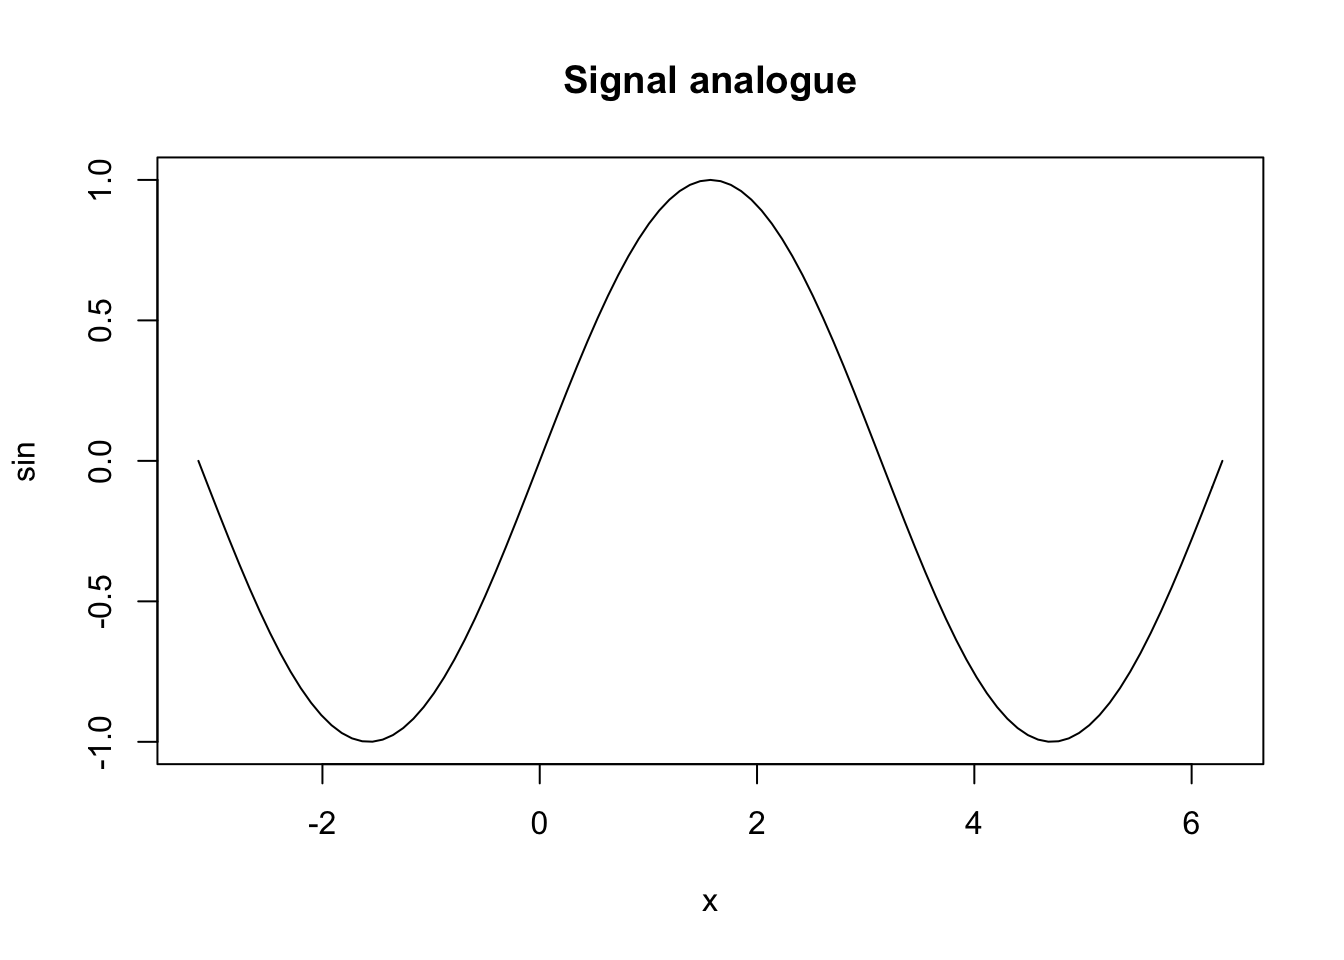
\includegraphics{traitement-video_files/figure-latex/unnamed-chunk-4-1} 

}

\caption{Fluctuation continue entre minimum et maximum}\label{fig:unnamed-chunk-4}
\end{figure}

\hypertarget{numuxe9rique-binaire}{%
\paragraph{Numérique : binaire}\label{numuxe9rique-binaire}}

0 ou 1, toute donnée est un entier, les valeurs interstitielles sont arrondies

\begin{figure}

{\centering 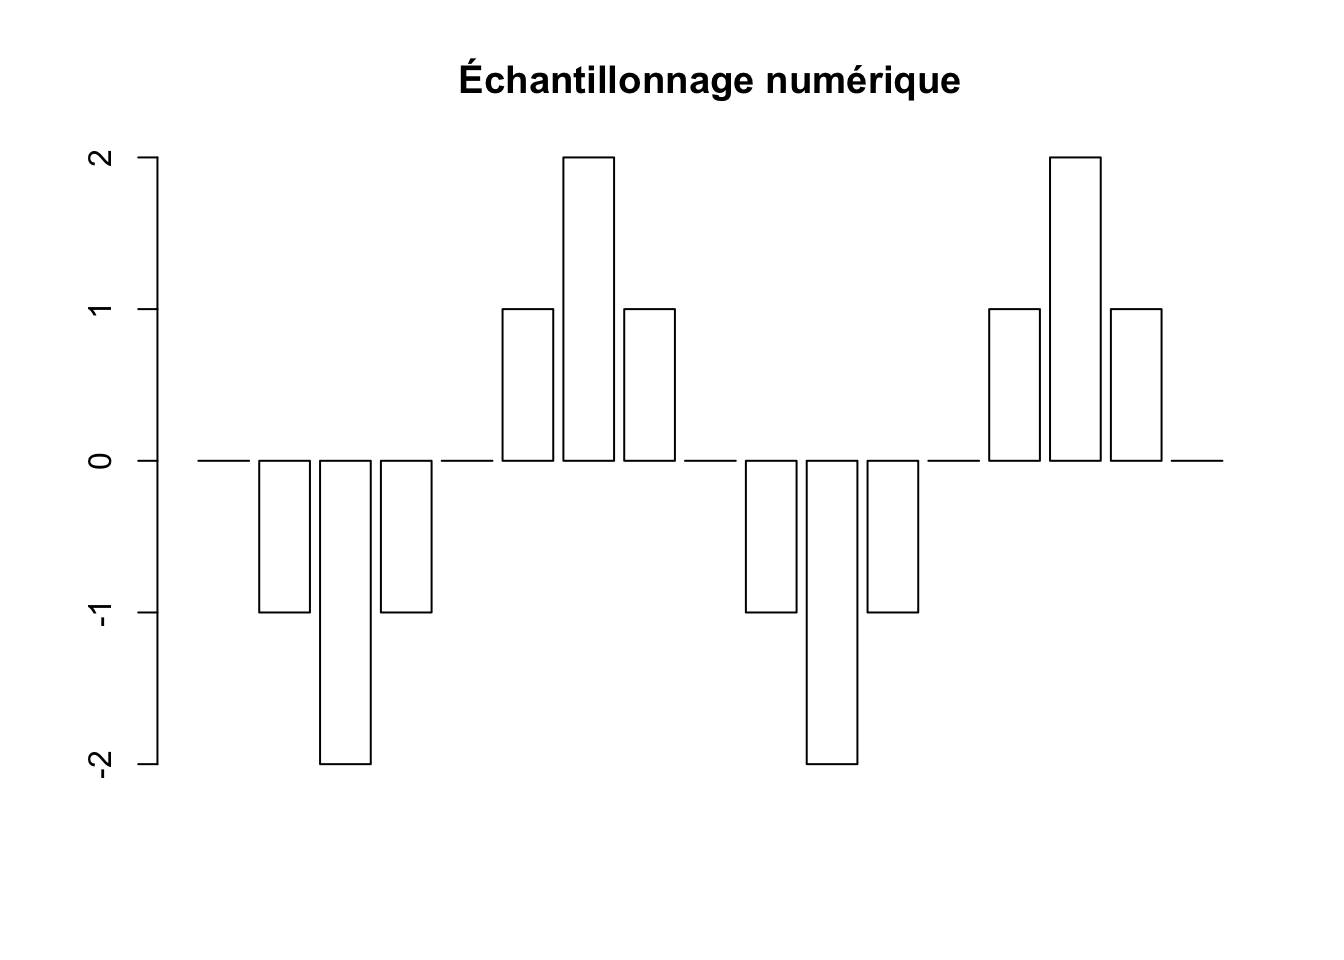
\includegraphics{traitement-video_files/figure-latex/unnamed-chunk-5-1} 

}

\caption{Binarisation des valeurs}\label{fig:unnamed-chunk-5}
\end{figure}

\hypertarget{usages}{%
\subsubsection{Usages}\label{usages}}

\begin{itemize}
\tightlist
\item
  \href{https://en.wikipedia.org/wiki/Video\#Analog_video}{Signaux analogues/digitaux}
\item
  \href{http://what-when-how.com/display-interfaces/basics-of-analog-and-digital-display-interfaces-part-1/}{Distinction}
\item
  \href{http://what-when-how.com/display-interfaces/basic-concepts-in-display-systems-part-1/}{principes d'affichage analogue}
\item
  \href{https://en.wikipedia.org/wiki/Analog_television}{Transmission télévisuelle analogue}
\item
  \href{https://github.com/sebpiq/cours-son-reseaux/blob/main/data-encodage.md}{Encodage binaire avancé}
\end{itemize}

\hypertarget{protocoles-de-transport}{%
\section{Protocoles de transport}\label{protocoles-de-transport}}

\url{https://en.wikipedia.org/wiki/Video}

\hypertarget{analogues}{%
\subsection{Analogues}\label{analogues}}

\hypertarget{composite}{%
\subsubsection{Composite}\label{composite}}

\begin{figure}
\centering
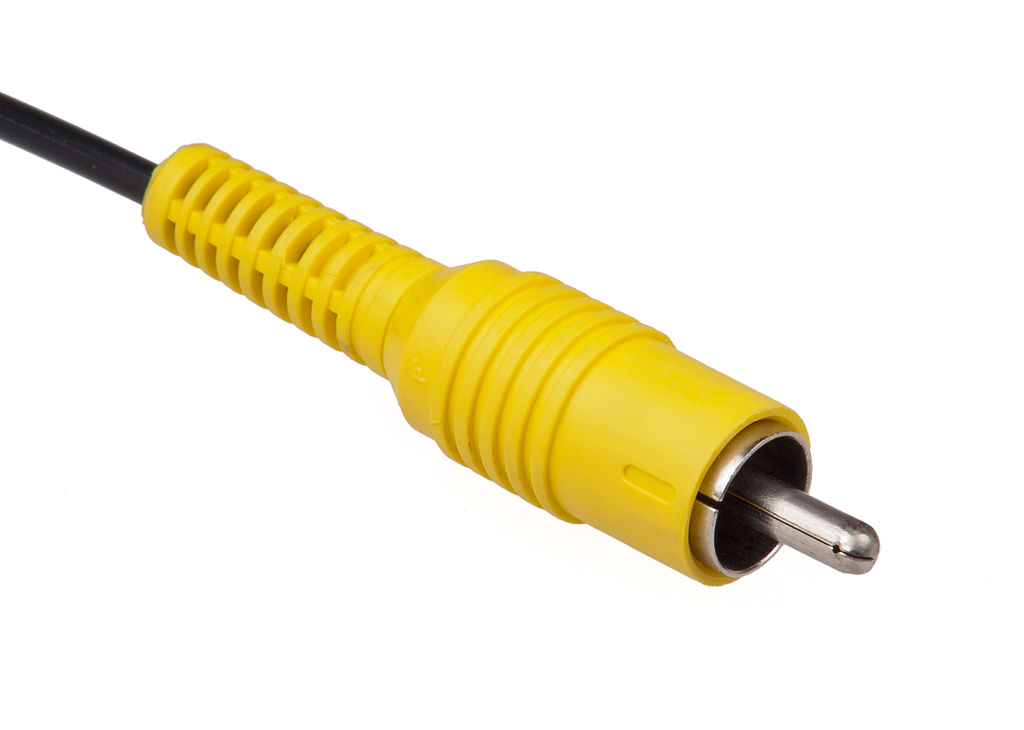
\includegraphics[width=0.5\textwidth,height=\textheight]{medias/lexique/signaux/analogue/composite.jpg}
\caption{Connecteur RCA pour signal \emph{composite}}
\end{figure}

\hypertarget{s-video}{%
\subsubsection{S-Video}\label{s-video}}

\begin{figure}
\centering
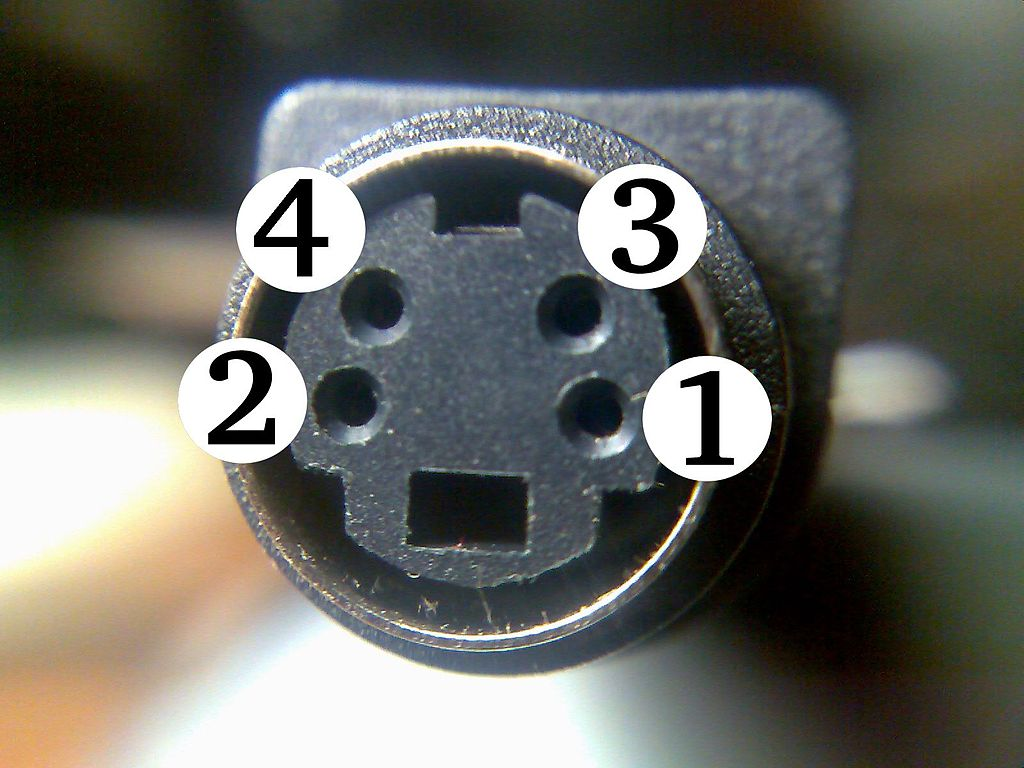
\includegraphics[width=0.5\textwidth,height=\textheight]{medias/lexique/signaux/analogue/svideo.jpg}
\caption{Connecteur pour signal \emph{S-Video}}
\end{figure}

\begin{itemize}
\tightlist
\item
  \emph{S-Vidéo} peut être converti passivement vers \emph{Composite} considérant une perte de qualité. (S-Vidéo \textgreater{} Composite)
\end{itemize}

\hypertarget{component}{%
\subsubsection{Component}\label{component}}

\begin{figure}
\centering
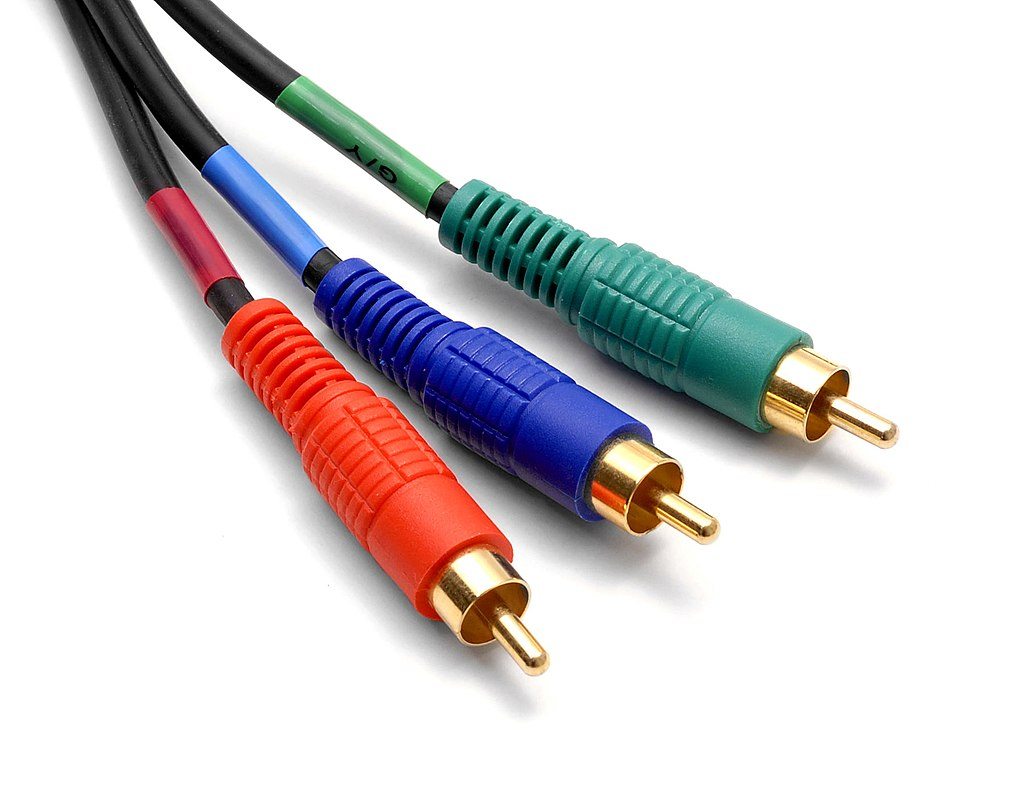
\includegraphics[width=0.5\textwidth,height=\textheight]{medias/lexique/signaux/analogue/component.jpg}
\caption{Connecteurs RCA pour signal \emph{Component}}
\end{figure}

\hypertarget{vga}{%
\subsubsection{VGA}\label{vga}}

\begin{figure}
\centering
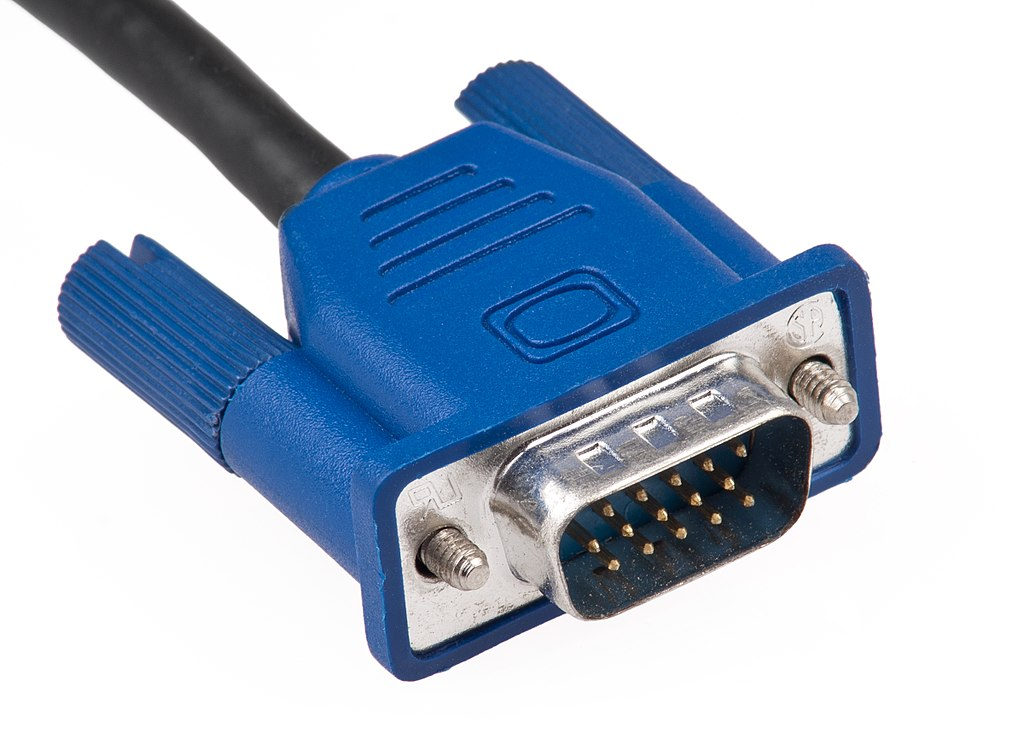
\includegraphics[width=0.5\textwidth,height=\textheight]{medias/lexique/signaux/analogue/vga.jpg}
\caption{Connecteur DE-15 pour signal VGA}
\end{figure}

\hypertarget{trrc}{%
\subsubsection{TRRC}\label{trrc}}

\begin{figure}
\centering
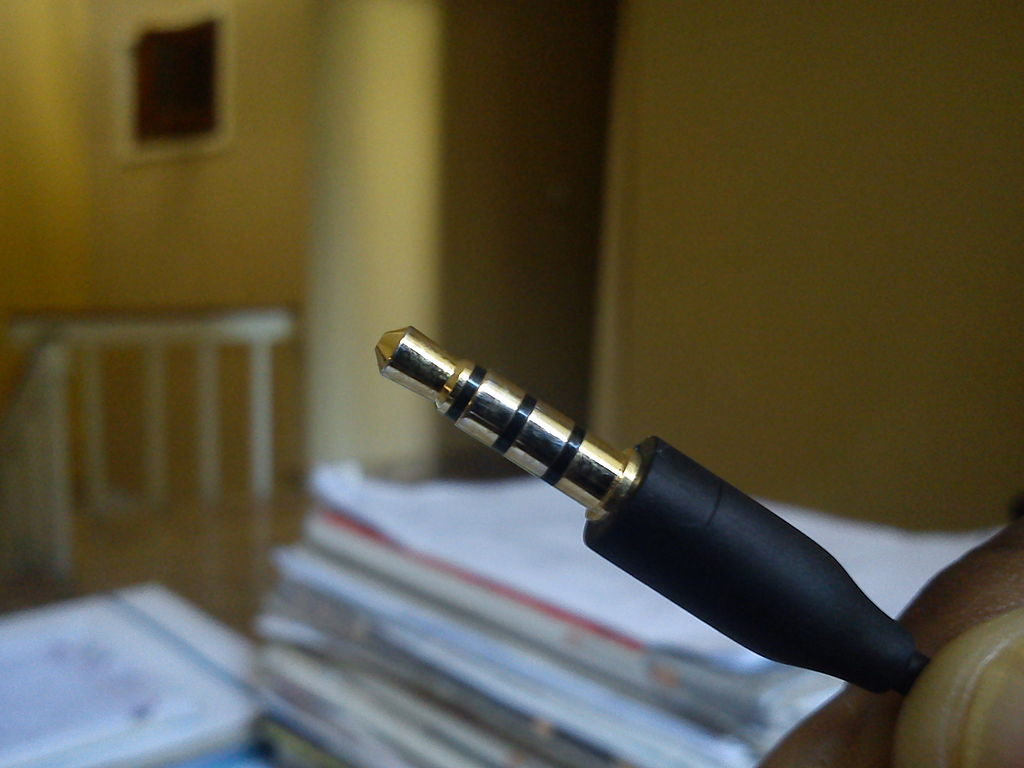
\includegraphics[width=0.5\textwidth,height=\textheight]{medias/lexique/signaux/analogue/3_5mm.jpg}
\caption{Connecteur TRRS pour signal composite et audio}
\end{figure}

\begin{itemize}
\tightlist
\item
  Composite et TRRC peuvent s'interchanger considérant la perte des canaux audio présents sur le TRRC
\end{itemize}

\hypertarget{numuxe9riques}{%
\subsection{Numériques}\label{numuxe9riques}}

\hypertarget{dvi}{%
\subsubsection{DVI}\label{dvi}}

\begin{figure}
\centering
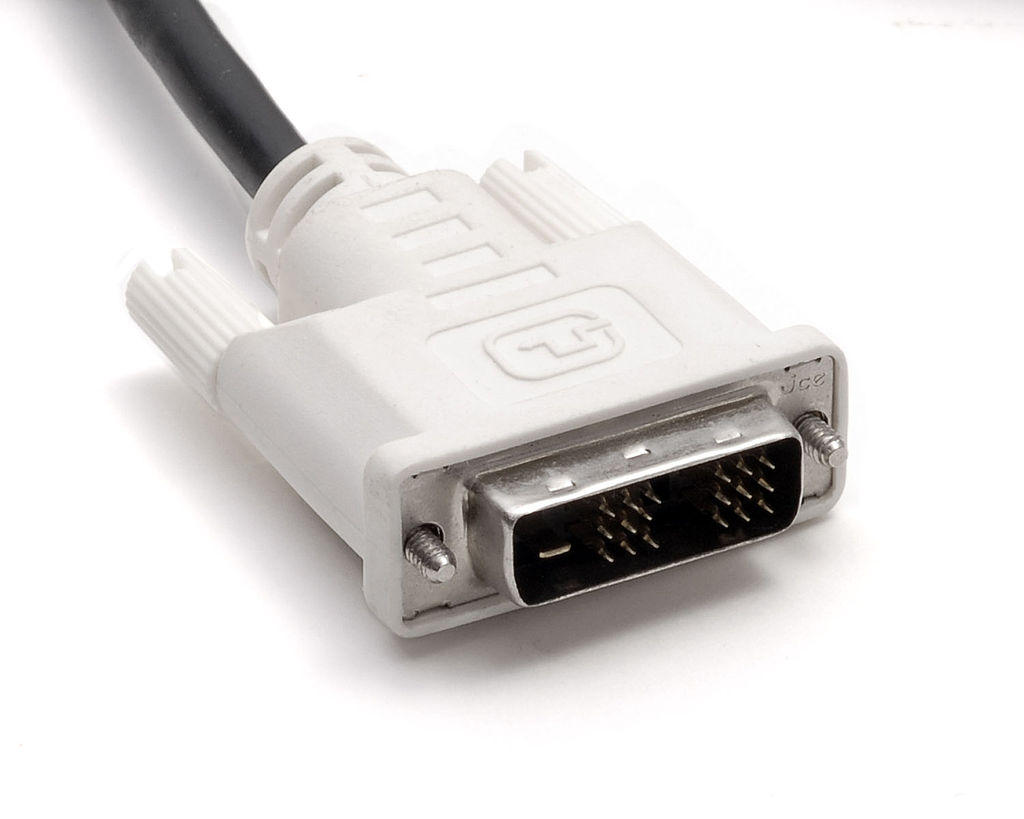
\includegraphics[width=0.5\textwidth,height=\textheight]{medias/lexique/signaux/numerique/dvi.jpg}
\caption{Connecteur DVI}
\end{figure}

\hypertarget{hdmi}{%
\subsubsection{HDMI}\label{hdmi}}

\begin{figure}
\centering
\includegraphics[width=0.5\textwidth,height=\textheight]{medias/lexique/signaux/numerique/hdmi.jpg}
\caption{Connecteur HDMI}
\end{figure}

\begin{itemize}
\tightlist
\item
  HDMI peut passer la vidéo vers DVI et vice versa, par contre le son est perdu dans cette conversion
\end{itemize}

\hypertarget{display-port}{%
\subsubsection{Display Port}\label{display-port}}

\begin{figure}
\centering
\includegraphics[width=0.5\textwidth,height=\textheight]{medias/lexique/signaux/numerique/displayport.jpg}
\caption{Connecteur Display Port}
\end{figure}

\begin{itemize}
\tightlist
\item
  \emph{Display Port} peut passer passivement vers HDMI ainsi que DVI. Le contraire n'est pas vrai. On ne peut pas passer de passivement de \emph{HDMI} vers \emph{Display port}.
\end{itemize}

\hypertarget{sdi}{%
\subsubsection{SDI}\label{sdi}}

\begin{figure}
\centering
\includegraphics[width=0.5\textwidth,height=\textheight]{medias/lexique/signaux/numerique/sdi.jpg}
\caption{Connecteur BNC pour signal SDI}
\end{figure}

\hypertarget{acquerir}{%
\chapter{Acquerir}\label{acquerir}}

\hypertarget{rapport-de-cadre-ratio}{%
\section{Rapport de cadre (Ratio)}\label{rapport-de-cadre-ratio}}

\begin{itemize}
\tightlist
\item
  S'écrit généralement en utilisant le deux point pour séparer la largeur de la hauteur.
\end{itemize}

\[
largeur : hauteur 
\]

Parfois on utilise aussi le barre de division

\[
largeur / hauteur 
\]

\begin{itemize}
\tightlist
\item
  Généralement exprimé avec ratio entier
\end{itemize}

\hypertarget{section-1}{%
\subsection{16:9}\label{section-1}}

\begin{itemize}
\tightlist
\item
  Ratio vidéo légèrement panoramique standard.
\end{itemize}

\begin{figure}
\centering
\includegraphics{medias/lexique/fullHD_16_9_1920x1080.png}
\caption{Full HD 16:9 1920x1080}
\end{figure}

\begin{figure}
\centering
\includegraphics{medias/lexique/barre_couleurs-1600x900.png}
\caption{barres de calibration}
\end{figure}

\hypertarget{section-2}{%
\subsection{4:3}\label{section-2}}

\begin{itemize}
\tightlist
\item
  ratio vidéo utilisé au temps des tubes cathodiques
\end{itemize}

\begin{figure}
\centering
\includegraphics{medias/lexique/NTSC_4_3_640x480.png}
\caption{NTSC 4:3}
\end{figure}

\begin{itemize}
\tightlist
\item
  Attention; ce format provenant du monde analogue et est soumis parfois des variations exotiques
  \url{https://en.wikipedia.org/wiki/Pixel_aspect_ratio\#Analog-to-digital_conversion}
\end{itemize}

\hypertarget{section-3}{%
\subsection{3:2}\label{section-3}}

\begin{itemize}
\item
  Ratio provenant du film \href{https://en.wikipedia.org/wiki/35_mm_format}{35mm} qui mesurait réellement 36×24 mm
\item
  Ratio généralement utilisé en photographie
\end{itemize}

\begin{figure}
\centering
\includegraphics{medias/lexique/Photo_3_2_2000x1333.png}
\caption{NTSC 4:3}
\end{figure}

\hypertarget{section-4}{%
\subsection{2,39:1}\label{section-4}}

\begin{itemize}
\tightlist
\item
  CinemaScope; \url{https://fr.wikipedia.org/wiki/CinemaScope}

  \begin{itemize}
  \tightlist
  \item
    Jadis, déformation optique au tournage ainsi qu'à la diffusion
  \end{itemize}
\end{itemize}

\begin{figure}
\centering
\includegraphics{medias/lexique/Cinemascope_2_39_1_2390x1000.png}
\caption{Carré 1:1}
\end{figure}

\begin{itemize}
\tightlist
\item
  Épique
\end{itemize}

\hypertarget{section-5}{%
\subsection{1:1}\label{section-5}}

\begin{itemize}
\tightlist
\item
  Ratio provenant de la photographie \href{https://fr.wikipedia.org/wiki/Appareil_photographique_de_moyen_format}{moyen format}
\end{itemize}

\begin{figure}
\centering
\includegraphics{medias/lexique/carre_1_1_1000x1000.png}
\caption{1:1 ratio}
\end{figure}

\begin{figure}
\centering
\includegraphics{medias/lexique/CubeMap_4096x4096.png}
\caption{1:1 Environnement sphérique \emph{Cube map}}
\end{figure}

\begin{itemize}
\tightlist
\item
  Utilie pour

  \begin{itemize}
  \tightlist
  \item
    texture vidéo
  \item
    \href{https://vioso.com/softedge-patterngenerator/domegrids/CubeMap_4096x4096.png}{Format dôme immersif}
  \end{itemize}
\end{itemize}

\hypertarget{guxe9nuxe9rateur-dimage-de-calibration}{%
\subsection{Générateur d'image de calibration}\label{guxe9nuxe9rateur-dimage-de-calibration}}

\begin{itemize}
\tightlist
\item
  interface web

  \begin{itemize}
  \tightlist
  \item
    \url{https://vioso.com/testpattern-generator/}
  \end{itemize}
\end{itemize}

\hypertarget{ruxe9fuxe9rences}{%
\subsection{Références}\label{ruxe9fuxe9rences}}

\begin{itemize}
\tightlist
\item
  \url{https://fr.wikipedia.org/wiki/Format_d\%27image}
\item
  \href{https://en.wikipedia.org/wiki/Display_aspect_ratio}{ratios image}
\item
  \href{https://en.wikipedia.org/wiki/Pixel_aspect_ratio}{ratios-pixels}
\end{itemize}

\hypertarget{physique-de-limagerie-numuxe9rique}{%
\section{Physique de l'imagerie numérique}\label{physique-de-limagerie-numuxe9rique}}

\hypertarget{le-systuxe8me-oculaire}{%
\subsection{Le système oculaire}\label{le-systuxe8me-oculaire}}

\begin{itemize}
\tightlist
\item
  \url{http://what-when-how.com/display-i/nterfaces/the-human-visual-system-display-interfaces-part-1/}
\end{itemize}

\hypertarget{numuxe9riser-la-lumiuxe8re-ruxe9fluxe9chie}{%
\subsection{Numériser la lumière réfléchie}\label{numuxe9riser-la-lumiuxe8re-ruxe9fluxe9chie}}

\begin{itemize}
\tightlist
\item
  \url{http://what-when-how.com/introduction-to-video-and-image-processing/image-acquisition-introduction-to-video-and-image-processing-part-1/}
\end{itemize}

\hypertarget{propriuxe9tuxe9s-de-limage-numuxe9rique}{%
\subsection{Propriétés de l'image numérique}\label{propriuxe9tuxe9s-de-limage-numuxe9rique}}

\begin{itemize}
\tightlist
\item
  \url{http://what-when-how.com/introduction-to-video-and-image-processing/image-acquisition-introduction-to-video-and-image-processing-part-2/}
\end{itemize}

\hypertarget{acquerir_captation}{%
\section{Acquisition vidéo numérique temps réel}\label{acquerir_captation}}

\hypertarget{sources-viduxe9o-obs}{%
\subsection{Sources vidéo OBS}\label{sources-viduxe9o-obs}}

\hypertarget{puxe9riphuxe9rique-de-capture-viduxe9o}{%
\subsubsection{Périphérique de capture vidéo}\label{puxe9riphuxe9rique-de-capture-viduxe9o}}

\begin{itemize}
\tightlist
\item
  Webcam
\item
  Carte de capture HDMI
\end{itemize}

\hypertarget{capture-duxe9cran}{%
\subsubsection{Capture d'écran}\label{capture-duxe9cran}}

\hypertarget{capture-de-fenuxeatre}{%
\subsubsection{Capture de fenêtre}\label{capture-de-fenuxeatre}}

\hypertarget{capture-de-contexte-gl-game-capture}{%
\subsubsection{Capture de contexte GL (Game capture)}\label{capture-de-contexte-gl-game-capture}}

\hypertarget{partage-de-texture-viduxe9o-spout-syphon}{%
\subsubsection{Partage de texture vidéo (Spout, Syphon)}\label{partage-de-texture-viduxe9o-spout-syphon}}

\hypertarget{camuxe9ra-virtuelle}{%
\subsubsection{Caméra virtuelle}\label{camuxe9ra-virtuelle}}

\hypertarget{navigateur}{%
\subsubsection{Navigateur}\label{navigateur}}

\hypertarget{tutoriels-obs-francophone-duxe9mystifiant-linterface}{%
\subsection{Tutoriels OBS francophone démystifiant l'interface}\label{tutoriels-obs-francophone-duxe9mystifiant-linterface}}

\begin{itemize}
\tightlist
\item
  \url{https://www.leterminal.fr/manuel-obs-studio/}
\item
  \url{https://maniacgeek.net/informatique/obs/utiliser-obs-guide/}
\item
  \url{https://sospc.name/obs-studio-tutoriel-mia/}
\end{itemize}

\hypertarget{echantillonner}{%
\chapter{Échantillonner}\label{echantillonner}}

\hypertarget{compression-du-signal}{%
\section{Compression du signal}\label{compression-du-signal}}

\begin{figure}

{\centering \includegraphics{traitement-video_files/figure-latex/unnamed-chunk-6-1} 

}

\caption{Qualificatif de compression vidéo}\label{fig:unnamed-chunk-6}
\end{figure}

\hypertarget{signal-viduxe9o-compressuxe9-vs-non-compressuxe9}{%
\subsection{Signal vidéo compressé vs non-compressé}\label{signal-viduxe9o-compressuxe9-vs-non-compressuxe9}}

\hypertarget{non-compressuxe9}{%
\subsubsection{Non compressé}\label{non-compressuxe9}}

\hypertarget{propriuxe9tuxe9s-du-signal-non-compressuxe9}{%
\paragraph{Propriétés du signal non Compressé}\label{propriuxe9tuxe9s-du-signal-non-compressuxe9}}

\begin{itemize}
\tightlist
\item
  Sans perte
\item
  Rapide pour effectuer des opérations graphique
\item
  Utilise beaucoup de mémoire
\end{itemize}

\[
data rate = color depth *  pixHorizontal * pixVertical * refresh frequency
\]

Se traduit vers :

\[
Débit = profondeur(bits)  * résolutionHorizontale * résolutionVerticale * cadence
\]

Un signal \textbf{fullhd 60p} non compressé corresponds au calcul suivant :

\[
24 * 1920 * 1080 * 60 = 2.98 Gbit/s.
\]

L'exemple ci-haut correspond à un échantillonnage de 24 bits, une résolution de 1920 pixels horizontaux par 1080 pixels verticaux et une cadence de 60 image progressive par secondes.

\hypertarget{usages-de-la-viduxe9o-non-compressuxe9e}{%
\paragraph{Usages de la vidéo non-compressée}\label{usages-de-la-viduxe9o-non-compressuxe9e}}

\begin{itemize}
\tightlist
\item
  \url{https://en.wikipedia.org/wiki/Uncompressed_video}
\end{itemize}

\hypertarget{compressuxe9}{%
\subsubsection{Compressé}\label{compressuxe9}}

Quand il y a compression, des instructions sont exécutées par le lecteur pour restituer l'image à temps.

La configuration de la compression vidéo est déterminée par différents facteurs

\begin{itemize}
\tightlist
\item
  L'usage
\item
  La mémoire disponible
\item
  La bande passante disponible
\item
  La présence de circuit dédié (encodage/décodage matériel)
\end{itemize}

\hypertarget{compression-sans-pertes-vs-destructive-losslesslossy}{%
\subsection{Compression sans pertes vs destructive (lossless/lossy)}\label{compression-sans-pertes-vs-destructive-losslesslossy}}

\hypertarget{encodage-viduxe9o-sans-perte---lossless}{%
\subsubsection{\texorpdfstring{\href{https://en.wikipedia.org/wiki/List_of_codecs\#Lossless_video_compression}{Encodage vidéo sans perte - \textbf{lossless}}}{Encodage vidéo sans perte - lossless}}\label{encodage-viduxe9o-sans-perte---lossless}}

La compression vise à réduire le poids.

Il est lourd d'écrire en détail chaque information.

\begin{verbatim}
[0xFFFFFF]
[0xFFFFFF]
[0xFFFFFF]
[0xFFFFFF]
[0xAA66EE]
\end{verbatim}

On peut compresser sans perte en opérationnalisant la redondance d'informations adjacente.

\begin{verbatim}
4*[0xFFFFFF]
1*[0xAA66EE]
\end{verbatim}

\hypertarget{caractuxe9ristiques}{%
\paragraph{Caractéristiques:}\label{caractuxe9ristiques}}

\begin{itemize}
\tightlist
\item
  Volumineux
\item
  Privilégié entre les opérations de rendu où l'intégrité de l'information est critique
\item
  Généralement plus facile à mettre en mémoire graphique (GPU)
\end{itemize}

\hypertarget{usages-1}{%
\paragraph{Usages}\label{usages-1}}

\begin{itemize}
\tightlist
\item
  Au sein d'un processus de production/post-production
\end{itemize}

\hypertarget{type-de-muxe9dias-lossless}{%
\paragraph{Type de médias lossless}\label{type-de-muxe9dias-lossless}}

\begin{itemize}
\tightlist
\item
  Apple Animation (QuickTime RLE)
\item
  CinemaDNG Raw (Adobe, Blackmagic)
\item
  séquence d'images (tiff, openexr)
\end{itemize}

\hypertarget{encodage-viduxe9o-destructif-lossy}{%
\subsubsection{\texorpdfstring{\href{https://en.wikipedia.org/wiki/List_of_codecs\#Lossy_compression_2}{Encodage vidéo destructif \textbf{lossy}}}{Encodage vidéo destructif lossy}}\label{encodage-viduxe9o-destructif-lossy}}

L'idée ici est de soustraire/compresser de la manière la plus transparente possible l'information la moins pertinente.
Des méthodes soustractives oeuvrant sur notre incapacité de percevoir certains détails sont employées (psycho cognitive).

\begin{itemize}
\tightlist
\item
  Ex.: le MP3

  \begin{itemize}
  \tightlist
  \item
    \url{https://ledgernote.com/blog/q-and-a/how-does-mp3-compression-work/}
  \end{itemize}
\end{itemize}

La compression peut s'opérer au sein d'une image (\textbf{intraframe}) ou au sein d'une séquence d'image (\textbf{interframe}).

Méthode de compressions applicables;

\hypertarget{intraframe}{%
\paragraph{\texorpdfstring{\href{http://users.cs.cf.ac.uk/Dave.Marshall/Multimedia/node248.html}{intraframe}}{intraframe}}\label{intraframe}}

\begin{itemize}
\tightlist
\item
  Toute l'image individuellement compressée dans chaque image.

  \begin{itemize}
  \tightlist
  \item
    prores, dnxHD, photoJpeg, Apple intermediate codec (aic), cineform, Hap\\
  \end{itemize}
\item
  Utile quand la tête de lecture fait des accès aléatoires dans le temps

  \begin{itemize}
  \tightlist
  \item
    Ex. Montage vidéo
  \end{itemize}
\item
  Généralement volumineux (chaque image du fichier vidéo existe )
\end{itemize}

\hypertarget{interframe}{%
\paragraph{\texorpdfstring{\href{http://users.cs.cf.ac.uk/Dave.Marshall/Multimedia/node249.htmlhttps://en.wikipedia.org/wiki/Inter_frame}{interframe}}{interframe}}\label{interframe}}

\begin{itemize}
\tightlist
\item
  image temporellement compressée, \href{http://dvd-hq.info/data_compression_3.php}{ce qui change}

  \begin{itemize}
  \tightlist
  \item
    \href{https://en.wikipedia.org/wiki/Video_compression_picture_types}{images: I (clef), P (\textless-) et B(\textless-\textgreater)}
  \item
    \href{https://en.wikipedia.org/wiki/Inter_frame\#/media/File:IPB_images_sequence.png}{GOP : group of picture}
  \end{itemize}
\item
  Utile en lecture linéaire, du début vers la fin
\item
  usage créatif de la compression

  \begin{itemize}
  \tightlist
  \item
    \href{https://www.youtube.com/watch?v=rMSsw4CZvKg}{1}
  \item
    \href{https://www.youtube.com/watch?v=rSmEOk5AiN0}{2}
  \item
    \href{https://www.youtube.com/watch?v=dNa0-xrKi3Q}{3}
  \end{itemize}
\end{itemize}

\hypertarget{type-de-compression-destructive}{%
\paragraph{Type de compression destructive}\label{type-de-compression-destructive}}

\begin{itemize}
\tightlist
\item
  proRes, dnxHD, cineform \footnote{Ces codecs sont généralement utilisés en postproduction et sont souvent confondus avec des \textbf{codecs lossless }.
    Ces codecs ont différentes moutures capables de combler différents besoins, du proxy (très compressé) vers le très peu compressé avec canal alpha (4:4:4:4).}
\item
  H.264\&VP8
\item
  HEVC\&VP9\\
\item
  HAP \& HAPQ
\end{itemize}

\hypertarget{lexique_encodage}{%
\section{Lexique de l'encodage}\label{lexique_encodage}}

\hypertarget{vocabulaire}{%
\subsection{Vocabulaire}\label{vocabulaire}}

\hypertarget{duxe9bit}{%
\subsubsection{Débit}\label{duxe9bit}}

Associé à la bande passante du signal, généralement exprimé en nombre de bits par seconde.

\begin{itemize}
\item
  1 bit{[}b{]} = 1xbit
\item
  1 octet{[}byte{]}{[}B{]} = 8xbits
\item
  Mbit/s -\textgreater{} mégabit par seconde
\item
  MBit/s -\textgreater{} mégaoctets (megabyte) par seconde
\item
  \href{https://en.wikipedia.org/wiki/Bit_rate\#Video}{Débit (bitrate)}
\item
  \url{http://what-when-how.com/introduction-to-video-and-image-processing/bits-bytes-and-binary-numbers-introduction-to-video-and-image-processing/}
\end{itemize}

\hypertarget{calculer-le-poids-bitrate}{%
\paragraph{Calculer le poids (bitrate)}\label{calculer-le-poids-bitrate}}

\begin{itemize}
\tightlist
\item
  \href{https://toolstud.io/video/filesize.php?imagewidth=1920\&imageheight=1080\&framerate=29.97\&timeduration=60\&timeunit=seconds}{calcul de grosseur de fichier}
\item
  \href{https://toolstud.io/video/bitrate.php?imagewidth=1\&imageheight=1\&colordepth=24\&framerate=29.97}{calcul de bitrate}
\end{itemize}

\hypertarget{canal-alpha-alpha-channel}{%
\subsubsection{\texorpdfstring{Canal alpha \emph{Alpha channel}}{Canal alpha Alpha channel}}\label{canal-alpha-alpha-channel}}

Canal dédié à la transparence.
Sa présence permet de composer des images en préservant les attributs de transparence.

\hypertarget{profondeur-duxe9chantillonnage}{%
\subsubsection{Profondeur d'échantillonnage}\label{profondeur-duxe9chantillonnage}}

\begin{itemize}
\tightlist
\item
  Profondeur de l'échantillonnage couleur

  \begin{itemize}
  \tightlist
  \item
    \href{https://en.wikipedia.org/wiki/Color_depth}{bit/canal}\\
  \end{itemize}
\item
  \href{https://en.wikipedia.org/wiki/Chroma_subsampling\#Sampling_systems_and_ratios}{chroma subsampling}

  \begin{itemize}
  \tightlist
  \item
    \href{https://upload.wikimedia.org/wikipedia/commons/0/06/Colorcomp.jpg}{4:4:4 vs 4:2:2 vs 4:2:0}
  \item
    \href{https://en.wikipedia.org/wiki/Alpha_compositing}{4:4:4 vs 4:4:4:4}
  \end{itemize}
\end{itemize}

\hypertarget{lexique_fichiers}{%
\section{Encodage/décodage de fichiers}\label{lexique_fichiers}}

L'encodage permet la lecture de fichiers et de flux vidéo.
L'encodage est déterminé par la configuration d'un codec dans un conteneur.

\hypertarget{format-dencodage-codecs}{%
\subsection{Format d'encodage (Codecs)}\label{format-dencodage-codecs}}

\begin{longtable}[]{@{}lll@{}}
\toprule
Codec & compression & usage\tabularnewline
\midrule
\endhead
H.264\&VP8 & intra \& inter & lecture\textless1080p\tabularnewline
HEVC\&VP9 & intra \& inter & lecture\textless4k\tabularnewline
proRes & intra & montage\tabularnewline
dnxHD & intra & montage\tabularnewline
HAP & intra & GPU\&SSD\tabularnewline
\bottomrule
\end{longtable}

\hypertarget{contenant-containers}{%
\subsection{Contenant (Containers)}\label{contenant-containers}}

\begin{longtable}[]{@{}ll@{}}
\toprule
nom & extension\tabularnewline
\midrule
\endhead
QuickTime & .mov\tabularnewline
Matroska & .mkv\tabularnewline
Mpeg4 & .mp4\tabularnewline
Windows Media Video & .wmv\tabularnewline
Audio Video Interleaved & .avi\tabularnewline
Theora & .ogv\tabularnewline
\bottomrule
\end{longtable}

\href{https://en.wikipedia.org/wiki/Comparison_of_video_container_formats}{wiki:Comparison\_of\_video\_container\_formats}

\hypertarget{formats-de-sauvegarde-et-archivage-des-muxe9dias}{%
\subsection{Formats de sauvegarde et archivage des médias}\label{formats-de-sauvegarde-et-archivage-des-muxe9dias}}

\hypertarget{pruxe9sentations-des-codecs-tim}{%
\subsubsection{Présentations des codecs TIM}\label{pruxe9sentations-des-codecs-tim}}

\url{https://cmontmorency365.sharepoint.com/:p:/s/TIM-TTP/EZJO9E0y6idAql7kKqGyKFQB--xsTpIiWADt1-m3hnbBgg?e=UQXaWB}

\hypertarget{pour-aller-plus-loin}{%
\subsubsection{Pour aller plus loin}\label{pour-aller-plus-loin}}

\begin{itemize}
\item
  pour des usages réguliers, voir :

  \begin{itemize}
  \tightlist
  \item
    FFmpeg Cookbook for Archivists \citep{kromer_FFmpegCookbookArchivists_2020}
  \item
    FFmpeg Cookbook par Greg Wessels \citep{wessels_FFmpegCookbook_2017}
  \end{itemize}
\item
  pour usages artistiques :

  \begin{itemize}
  \tightlist
  \item
    FFmpeg artschool \citep{associationofmovingimagearchivists_FFmpegArtschool_2020}
  \end{itemize}
\end{itemize}

\hypertarget{traiter}{%
\chapter{Traiter}\label{traiter}}

\hypertarget{vocabulaire-du-traitement-viduxe9o}{%
\section{Vocabulaire du traitement vidéo}\label{vocabulaire-du-traitement-viduxe9o}}

\hypertarget{pixel}{%
\subsection{Pixel}\label{pixel}}

Unité d'information encodée

Peut contenir une couleur\\
dans certain cas de la transparence.

Souvent utilisé en matrices pour afficher un signal vidéo.

Peut produire:

\begin{itemize}
\tightlist
\item
  Couleurs sur écran
\item
  Projection vidéo
\item
  Lumière pour espace
\end{itemize}

\hypertarget{matrice}{%
\subsection{Matrice}\label{matrice}}

Organisation multidimensionnelles de pixels.

\url{https://thebookofshaders.com/08//?lan=fr}

\begin{figure}
\centering
\includegraphics{medias/traiter/figures/dia_matrice_RGB.png}
\caption{Matrice 3 dimensions RGB}
\end{figure}

\begin{figure}
\centering
\includegraphics{medias/traiter/figures/dia_matrice_RGBA.png}
\caption{Matrice 4 dimensions RGBA}
\end{figure}

\hypertarget{traitement-matriciel}{%
\subsubsection{Traitement matriciel}\label{traitement-matriciel}}

\begin{itemize}
\tightlist
\item
  \url{http://what-when-how.com/introduction-to-video-and-image-processing/neighborhood-processing-introduction-to-video-and-image-processing-part-2/}
\end{itemize}

\hypertarget{texture}{%
\subsection{Texture}\label{texture}}

\url{https://thebookofshaders.com/09/?lan=fr}

\hypertarget{transformations-guxe9omuxe9triques}{%
\section{Transformations géométriques}\label{transformations-guxe9omuxe9triques}}

Affecte-le contenant de la texture. Nommé \emph{Vertex} dans le langage nuanciers \emph{shaders}

\begin{itemize}
\tightlist
\item
  \url{http://what-when-how.com/introduction-to-video-and-image-processing/geometric-transformations-introduction-to-video-and-image-processing-part-1/}
\end{itemize}

\hypertarget{position}{%
\subsection{Position}\label{position}}

\begin{figure}
\centering
\includegraphics{medias/traiter/figures/dia_transfogeo_position.png}
\caption{Transformation positionnel, translation}
\end{figure}

\hypertarget{rotation}{%
\subsection{Rotation}\label{rotation}}

\begin{figure}
\centering
\includegraphics{medias/traiter/figures/dia_transfogeo_rotation.png}
\caption{Transformation positionnel, rotation}
\end{figure}

\hypertarget{uxe9chelle}{%
\subsection{Échelle}\label{uxe9chelle}}

\begin{figure}
\centering
\includegraphics{medias/traiter/figures/dia_transfogeo_echelle.png}
\caption{Transformation positionnel, échelle}
\end{figure}

\hypertarget{dimensions}{%
\subsection{Dimensions}\label{dimensions}}

\begin{figure}
\centering
\includegraphics{medias/traiter/figures/dia_transfogeo_dimensions.png}
\caption{Transformation positionnel, dimensions}
\end{figure}

\hypertarget{rogner}{%
\subsection{Rogner}\label{rogner}}

\begin{figure}
\centering
\includegraphics{medias/traiter/figures/dia_transfogeo_rogner.png}
\caption{Transformation positionnel, dimensions}
\end{figure}

\hypertarget{distorsion}{%
\subsection{Distorsion}\label{distorsion}}

\begin{figure}
\centering
\includegraphics{medias/traiter/figures/dia_transfogeo_distortion.png}
\caption{Transformation positionnel, distortion}
\end{figure}

\hypertarget{altuxe9ration-des-pixels}{%
\section{Altération des pixels}\label{altuxe9ration-des-pixels}}

Affecte le contenu de la texture.
Affecte les \emph{Fragments} , nuances, \emph{shaders}

\begin{itemize}
\tightlist
\item
  \url{http://what-when-how.com/introduction-to-video-and-image-processing/visual-effects-introduction-to-video-and-image-processing-part-1/}
\end{itemize}

\hypertarget{luminance}{%
\subsection{Luminance}\label{luminance}}

\hypertarget{contraste}{%
\subsubsection{Contraste}\label{contraste}}

\begin{figure}

{\centering \subfloat[-2.00\label{fig:unnamed-chunk-7-1}]{\includegraphics[width=0.14\linewidth]{medias/traiter/fx_obs/cc-contrast/01_-2} }\subfloat[-1.00\label{fig:unnamed-chunk-7-2}]{\includegraphics[width=0.14\linewidth]{medias/traiter/fx_obs/cc-contrast/02_-1} }\subfloat[-0.50\label{fig:unnamed-chunk-7-3}]{\includegraphics[width=0.14\linewidth]{medias/traiter/fx_obs/cc-contrast/03_-05} }\subfloat[0\label{fig:unnamed-chunk-7-4}]{\includegraphics[width=0.14\linewidth]{medias/traiter/fx_obs/cc-contrast/04_0} }\subfloat[1.00\label{fig:unnamed-chunk-7-5}]{\includegraphics[width=0.14\linewidth]{medias/traiter/fx_obs/cc-contrast/05_05} }\subfloat[2.00\label{fig:unnamed-chunk-7-6}]{\includegraphics[width=0.14\linewidth]{medias/traiter/fx_obs/cc-contrast/06_1} }\subfloat[3.00\label{fig:unnamed-chunk-7-7}]{\includegraphics[width=0.14\linewidth]{medias/traiter/fx_obs/cc-contrast/07_2} }

}

\caption{Plage d'influence du paramètre **contraste** sur grille de calibration couleur}\label{fig:unnamed-chunk-7}
\end{figure}

\begin{itemize}
\tightlist
\item
  \url{https://www.rochester.edu/newscenter/microscopic-eye-movements-affect-how-we-see-contrast-358802/}
\end{itemize}

\hypertarget{gamma}{%
\subsubsection{Gamma}\label{gamma}}

\begin{figure}

{\centering \subfloat[-3\label{fig:unnamed-chunk-8-1}]{\includegraphics[width=0.14\linewidth]{medias/traiter/fx_obs/cc-gamma/01_-3} }\subfloat[-2\label{fig:unnamed-chunk-8-2}]{\includegraphics[width=0.14\linewidth]{medias/traiter/fx_obs/cc-gamma/02_-2} }\subfloat[-1\label{fig:unnamed-chunk-8-3}]{\includegraphics[width=0.14\linewidth]{medias/traiter/fx_obs/cc-gamma/03_-1} }\subfloat[0\label{fig:unnamed-chunk-8-4}]{\includegraphics[width=0.14\linewidth]{medias/traiter/fx_obs/cc-gamma/04_0} }\subfloat[1\label{fig:unnamed-chunk-8-5}]{\includegraphics[width=0.14\linewidth]{medias/traiter/fx_obs/cc-gamma/05_1} }\subfloat[2\label{fig:unnamed-chunk-8-6}]{\includegraphics[width=0.14\linewidth]{medias/traiter/fx_obs/cc-gamma/06_2} }\subfloat[3\label{fig:unnamed-chunk-8-7}]{\includegraphics[width=0.14\linewidth]{medias/traiter/fx_obs/cc-gamma/07_3} }

}

\caption{Plage d'influence du paramètre **gamma** sur grille de calibration couleur}\label{fig:unnamed-chunk-8}
\end{figure}

\hypertarget{luminosituxe9}{%
\subsubsection{Luminosité}\label{luminosituxe9}}

\emph{Brightness}

\begin{figure}

{\centering \subfloat[-1.00\label{fig:unnamed-chunk-9-1}]{\includegraphics[width=0.14\linewidth]{medias/traiter/fx_obs/cc-brightness/01} }\subfloat[-0.50\label{fig:unnamed-chunk-9-2}]{\includegraphics[width=0.14\linewidth]{medias/traiter/fx_obs/cc-brightness/02} }\subfloat[-0.25\label{fig:unnamed-chunk-9-3}]{\includegraphics[width=0.14\linewidth]{medias/traiter/fx_obs/cc-brightness/03} }\subfloat[0.00\label{fig:unnamed-chunk-9-4}]{\includegraphics[width=0.14\linewidth]{medias/traiter/fx_obs/cc-brightness/04} }\subfloat[0.25\label{fig:unnamed-chunk-9-5}]{\includegraphics[width=0.14\linewidth]{medias/traiter/fx_obs/cc-brightness/05} }\subfloat[0.50\label{fig:unnamed-chunk-9-6}]{\includegraphics[width=0.14\linewidth]{medias/traiter/fx_obs/cc-brightness/06} }\subfloat[1.00\label{fig:unnamed-chunk-9-7}]{\includegraphics[width=0.14\linewidth]{medias/traiter/fx_obs/cc-brightness/07} }

}

\caption{Influence du paramètre **Luminosité** sur grille de calibration couleur}\label{fig:unnamed-chunk-9}
\end{figure}

\begin{itemize}
\tightlist
\item
  \url{http://what-when-how.com/introduction-to-video-and-image-processing/point-processing-introduction-to-video-and-image-processing-part-1/}
\end{itemize}

\hypertarget{couleurs}{%
\subsection{Couleurs}\label{couleurs}}

\hypertarget{saturation}{%
\subsubsection{Saturation}\label{saturation}}

\begin{figure}

{\centering \subfloat[-1.00\label{fig:unnamed-chunk-10-1}]{\includegraphics[width=0.14\linewidth]{medias/traiter/fx_obs/cc-saturation/01} }\subfloat[-0.50\label{fig:unnamed-chunk-10-2}]{\includegraphics[width=0.14\linewidth]{medias/traiter/fx_obs/cc-saturation/02} }\subfloat[-0.25\label{fig:unnamed-chunk-10-3}]{\includegraphics[width=0.14\linewidth]{medias/traiter/fx_obs/cc-saturation/03} }\subfloat[0.00\label{fig:unnamed-chunk-10-4}]{\includegraphics[width=0.14\linewidth]{medias/traiter/fx_obs/cc-saturation/04} }\subfloat[1\label{fig:unnamed-chunk-10-5}]{\includegraphics[width=0.14\linewidth]{medias/traiter/fx_obs/cc-saturation/05} }\subfloat[3\label{fig:unnamed-chunk-10-6}]{\includegraphics[width=0.14\linewidth]{medias/traiter/fx_obs/cc-saturation/06} }\subfloat[5\label{fig:unnamed-chunk-10-7}]{\includegraphics[width=0.14\linewidth]{medias/traiter/fx_obs/cc-saturation/07} }

}

\caption{Plage d'influence du paramètre **saturation** sur grille de calibration couleur}\label{fig:unnamed-chunk-10}
\end{figure}

\hypertarget{duxe9calage-de-teinte}{%
\subsubsection{Décalage de teinte}\label{duxe9calage-de-teinte}}

\emph{Hue}

\begin{figure}

{\centering \subfloat[-180\label{fig:unnamed-chunk-11-1}]{\includegraphics[width=0.14\linewidth]{medias/traiter/fx_obs/cc-hue/01} }\subfloat[-120\label{fig:unnamed-chunk-11-2}]{\includegraphics[width=0.14\linewidth]{medias/traiter/fx_obs/cc-hue/02} }\subfloat[-60\label{fig:unnamed-chunk-11-3}]{\includegraphics[width=0.14\linewidth]{medias/traiter/fx_obs/cc-hue/03} }\subfloat[0\label{fig:unnamed-chunk-11-4}]{\includegraphics[width=0.14\linewidth]{medias/traiter/fx_obs/cc-hue/04} }\subfloat[60\label{fig:unnamed-chunk-11-5}]{\includegraphics[width=0.14\linewidth]{medias/traiter/fx_obs/cc-hue/05} }\subfloat[120\label{fig:unnamed-chunk-11-6}]{\includegraphics[width=0.14\linewidth]{medias/traiter/fx_obs/cc-hue/06} }\subfloat[180\label{fig:unnamed-chunk-11-7}]{\includegraphics[width=0.14\linewidth]{medias/traiter/fx_obs/cc-hue/07} }

}

\caption{Décalage de la teinte par incrément de 60 degrés}\label{fig:unnamed-chunk-11}
\end{figure}

\hypertarget{nuance-des-couleurs}{%
\subsubsection{Nuance des couleurs}\label{nuance-des-couleurs}}

LUT

\begin{itemize}
\item
  \url{https://github.com/Pomax/LUT-builder}
\item
  \url{https://i0.wp.com/thelandofcolor.com/wp-content/uploads/2010/03/HSL-Cone-Graphic.jpg?resize=550\%2C546}
\end{itemize}

\hypertarget{niveau-des-couleurs}{%
\subsubsection{Niveau des couleurs}\label{niveau-des-couleurs}}

\hypertarget{repruxe9sentation-numuxe9rique-de-la-couleur}{%
\subsubsection{Représentation numérique de la couleur}\label{repruxe9sentation-numuxe9rique-de-la-couleur}}

\begin{itemize}
\tightlist
\item
  \url{https://thebookofshaders.com/06/?lan=fr}
\end{itemize}

\hypertarget{sythuxe8se-de-la-couleurs}{%
\subsubsection{Sythèse de la couleurs}\label{sythuxe8se-de-la-couleurs}}

\begin{itemize}
\item
  \url{http://bech.free.fr/docs/colorim.htm}
\item
  \url{https://fr.wikipedia.org/wiki/Synth\%C3\%A8se_additive}
\end{itemize}

\hypertarget{additive}{%
\paragraph{Additive}\label{additive}}

à l'écran (RGB): additif

\hypertarget{soustractive}{%
\paragraph{Soustractive}\label{soustractive}}

à l'impression (CMYK) : soustractif

En lumière (filtre) : soustractif

\hypertarget{espace-couleurs}{%
\subsubsection{Espace couleurs}\label{espace-couleurs}}

\hypertarget{couleurs-et-longueurs-donde}{%
\subsubsection{Couleurs et longueurs d'onde}\label{couleurs-et-longueurs-donde}}

\begin{itemize}
\tightlist
\item
  \url{http://what-when-how.com/display-interfaces/fundamentals-of-color-display-interfaces-part-1/}
\item
  Perception de la chaleur d'une image

  \begin{itemize}
  \tightlist
  \item
    \url{http://what-when-how.com/display-interfaces/fundamentals-of-color-display-interfaces-part-2/}
  \end{itemize}
\item
  \url{http://what-when-how.com/introduction-to-video-and-image-processing/color-images-introduction-to-video-and-image-processing-part-1/}
\item
  \url{http://what-when-how.com/introduction-to-video-and-image-processing/color-images-introduction-to-video-and-image-processing-part-2/}
\item
  \url{http://what-when-how.com/introduction-to-video-and-image-processing/color-images-introduction-to-video-and-image-processing-part-3/}
\end{itemize}

\hypertarget{incrustation-dimage}{%
\subsection{Incrustation d'image}\label{incrustation-dimage}}

\hypertarget{opacituxe9}{%
\subsubsection{Opacité}\label{opacituxe9}}

\begin{figure}

{\centering \subfloat[1.00\label{fig:unnamed-chunk-12-1}]{\includegraphics[width=0.16\linewidth]{medias/traiter/fx_obs/cc-opacity/01} }\subfloat[0.75\label{fig:unnamed-chunk-12-2}]{\includegraphics[width=0.16\linewidth]{medias/traiter/fx_obs/cc-opacity/02} }\subfloat[0.50\label{fig:unnamed-chunk-12-3}]{\includegraphics[width=0.16\linewidth]{medias/traiter/fx_obs/cc-opacity/03} }\subfloat[0.25\label{fig:unnamed-chunk-12-4}]{\includegraphics[width=0.16\linewidth]{medias/traiter/fx_obs/cc-opacity/04} }\subfloat[0.0\label{fig:unnamed-chunk-12-5}]{\includegraphics[width=0.16\linewidth]{medias/traiter/fx_obs/cc-opacity/05} }

}

\caption{Dimminution de opacité}\label{fig:unnamed-chunk-12}
\end{figure}

\hypertarget{lumakey}{%
\subsubsection{Lumakey}\label{lumakey}}

\hypertarget{seuil-maximum}{%
\paragraph{Seuil Maximum}\label{seuil-maximum}}

Si la luminance du pixel est plus grande que le seuil maximum le pixel est transparent.

\begin{figure}

{\centering \subfloat[Nul\label{fig:unnamed-chunk-13-1}]{\includegraphics[width=0.16\linewidth]{medias/traiter/fx_obs/luma-max/01} }\subfloat[1.00\label{fig:unnamed-chunk-13-2}]{\includegraphics[width=0.16\linewidth]{medias/traiter/fx_obs/luma-max/02} }\subfloat[0.75\label{fig:unnamed-chunk-13-3}]{\includegraphics[width=0.16\linewidth]{medias/traiter/fx_obs/luma-max/03} }\subfloat[0.50\label{fig:unnamed-chunk-13-4}]{\includegraphics[width=0.16\linewidth]{medias/traiter/fx_obs/luma-max/04} }\subfloat[0.25\label{fig:unnamed-chunk-13-5}]{\includegraphics[width=0.16\linewidth]{medias/traiter/fx_obs/luma-max/05} }\subfloat[0.0\label{fig:unnamed-chunk-13-6}]{\includegraphics[width=0.16\linewidth]{medias/traiter/fx_obs/luma-max/06} }

}

\caption{Incrustation en luminance via seuil maximum}\label{fig:unnamed-chunk-13}
\end{figure}

\hypertarget{seuil-minimum}{%
\paragraph{Seuil Minimum}\label{seuil-minimum}}

Si la luminance du pixel est plus petite que le seuil minimum le pixel est transparent

\begin{figure}

{\centering \subfloat[Nul\label{fig:unnamed-chunk-14-1}]{\includegraphics[width=0.16\linewidth]{medias/traiter/fx_obs/luma-min/01} }\subfloat[0.00\label{fig:unnamed-chunk-14-2}]{\includegraphics[width=0.16\linewidth]{medias/traiter/fx_obs/luma-min/02} }\subfloat[0.25\label{fig:unnamed-chunk-14-3}]{\includegraphics[width=0.16\linewidth]{medias/traiter/fx_obs/luma-min/03} }\subfloat[0.50\label{fig:unnamed-chunk-14-4}]{\includegraphics[width=0.16\linewidth]{medias/traiter/fx_obs/luma-min/04} }\subfloat[0.75\label{fig:unnamed-chunk-14-5}]{\includegraphics[width=0.16\linewidth]{medias/traiter/fx_obs/luma-min/05} }\subfloat[1.00\label{fig:unnamed-chunk-14-6}]{\includegraphics[width=0.16\linewidth]{medias/traiter/fx_obs/luma-min/06} }

}

\caption{Incrustation en luminance via seuil minimum}\label{fig:unnamed-chunk-14}
\end{figure}

\hypertarget{chromakey}{%
\subsubsection{Chromakey}\label{chromakey}}

Transparence via seuils de chrominance

\hypertarget{utilisation-de-muxe9moire-tampon}{%
\section{Utilisation de mémoire tampon}\label{utilisation-de-muxe9moire-tampon}}

Traitement utilisant la mémoire pour mettre en tampon des images vidéo et effectuer des opérations temporelles sur celles-ci.

\hypertarget{duxe9lais}{%
\subsection{Délais}\label{duxe9lais}}

Lecture à postériori d'une séquence ou d'un flux capté

\hypertarget{ruxe9troaction-feedback}{%
\subsection{Rétroaction (feedback)}\label{ruxe9troaction-feedback}}

Réinjection du signal diffusé dans le signal diffusé

\hypertarget{programmer}{%
\chapter{Programmer}\label{programmer}}

\hypertarget{fonctions-du-traitement-viduxe9o-temps-ruxe9el}{%
\section{Fonctions du traitement vidéo temps réel}\label{fonctions-du-traitement-viduxe9o-temps-ruxe9el}}

Exploitation des fonctions des logiciels de traitement vidéo en temps réel

\hypertarget{rendu-opengl}{%
\subsection{Rendu OpenGL}\label{rendu-opengl}}

\url{https://openframeworks.cc/ofBook/chapters/openGL.html}

\url{https://www.tomdalling.com/blog/modern-opengl/08-even-more-lighting-directional-lights-spotlights-multiple-lights/}

\hypertarget{utilisation-de-nuanciers-shaders}{%
\section{Utilisation de nuanciers (shaders)}\label{utilisation-de-nuanciers-shaders}}

\hypertarget{traiter_logiciels}{%
\subsection{Logiciels de traitement vidéo interactif en temps réel}\label{traiter_logiciels}}

Traitement visuel en temps réel à l'aide d'effets et de logiciels de programmation multimédia.

\hypertarget{programmation-nodale}{%
\subsection{Programmation nodale}\label{programmation-nodale}}

\hypertarget{libres-et-gratuits}{%
\subsection{Libres et gratuits}\label{libres-et-gratuits}}

\begin{itemize}
\tightlist
\item
  Open Broadcast Studio

  \begin{itemize}
  \tightlist
  \item
    obs-ninja
  \item
    obs-websocket
  \item
  \end{itemize}
\end{itemize}

\hypertarget{programmer_grab}{%
\section{Programmation de la captation}\label{programmer_grab}}

\hypertarget{programmer_logiciels}{%
\section{Logiciels de programmation}\label{programmer_logiciels}}

\begin{itemize}
\tightlist
\item
  glsl
\end{itemize}

\hypertarget{programmation-deffets-temps-ruxe9el}{%
\section{Programmation d'effets temps réel}\label{programmation-deffets-temps-ruxe9el}}

\hypertarget{nuanceurs-shaders}{%
\subsection{Nuanceurs (shaders)\,:}\label{nuanceurs-shaders}}

\url{https://thebookofshaders.com/01/?lan=fr}

\hypertarget{vertex-pixel-et-guxe9omuxe9trie}{%
\subsubsection{vertex, pixel et géométrie}\label{vertex-pixel-et-guxe9omuxe9trie}}

\hypertarget{usages-2}{%
\subsubsection{Usages}\label{usages-2}}

\url{https://thebookofshaders.com/00/?lan=fr}

\hypertarget{lumiuxe8re}{%
\paragraph{lumière}\label{lumiuxe8re}}

\hypertarget{texture-1}{%
\paragraph{texture}\label{texture-1}}

Noise : \url{https://thebookofshaders.com/11/}

\url{https://thebookofshaders.com/12/}

\hypertarget{fumuxe9e}{%
\paragraph{fumée}\label{fumuxe9e}}

\url{https://thebookofshaders.com/13/}

\hypertarget{programmation-de-compositions-visuelles-guxe9nuxe9ratives}{%
\section{Programmation de compositions visuelles génératives}\label{programmation-de-compositions-visuelles-guxe9nuxe9ratives}}

\url{https://thebookofshaders.com/05/?lan=fr}
\url{https://thebookofshaders.com/10/?lan=fr}

\hypertarget{interagir}{%
\chapter{Interagir}\label{interagir}}

\hypertarget{lecture}{%
\section{Lecture}\label{lecture}}

\hypertarget{position-1}{%
\subsection{Position}\label{position-1}}

\hypertarget{boucle}{%
\subsection{Boucle}\label{boucle}}

\hypertarget{vitesse}{%
\subsection{Vitesse}\label{vitesse}}

\hypertarget{contruxf4ler-de-la-tuxeate-de-lecture-viduxe9o}{%
\subsection{Contrôler de la tête de lecture vidéo}\label{contruxf4ler-de-la-tuxeate-de-lecture-viduxe9o}}

\hypertarget{montage-temps-ruxe9el}{%
\subsection{Montage temps réel}\label{montage-temps-ruxe9el}}

\hypertarget{gestion-de-banques-dimages}{%
\subsection{Gestion de banques d'images}\label{gestion-de-banques-dimages}}

\hypertarget{effets-visuels-et-filtres-applicables-en-temps-ruxe9el-sur-des-matuxe9riaux-visuels}{%
\section{Effets visuels et filtres applicables en temps réel sur des matériaux visuels}\label{effets-visuels-et-filtres-applicables-en-temps-ruxe9el-sur-des-matuxe9riaux-visuels}}

\hypertarget{flot-de-donnuxe9es-entre-les-objets-du-logiciel}{%
\section{Flot de données entre les objets du logiciel}\label{flot-de-donnuxe9es-entre-les-objets-du-logiciel}}

\hypertarget{interagir_interfaces}{%
\section{Utilisation d'interfaces de contrôle interactives}\label{interagir_interfaces}}

\hypertarget{interagir_protocoles}{%
\section{Communication via protocoles paramétriques temps réel}\label{interagir_protocoles}}

\url{https://github.com/sebpiq/cours-son-reseaux/blob/main/applications-audio.md}

\hypertarget{protocole_osc}{%
\subsection{Open sound control (OSC)}\label{protocole_osc}}

\hypertarget{protocole_websocket}{%
\subsection{Websocket}\label{protocole_websocket}}

\hypertarget{protocole_midi}{%
\subsection{MIDI}\label{protocole_midi}}

\hypertarget{protocole_dmx}{%
\subsection{DMX}\label{protocole_dmx}}

\hypertarget{protocole_artnet}{%
\subsection{ArtNet}\label{protocole_artnet}}

\begin{itemize}
\tightlist
\item
  \url{https://openframeworks.cc/ofBook/chapters/image_processing_computer_vision.html}
\item
  \url{http://szeliski.org/Book/}
\end{itemize}

\hypertarget{usages-de-capture-viduxe9o-temps-ruxe9el}{%
\section{Usages de capture vidéo temps réel}\label{usages-de-capture-viduxe9o-temps-ruxe9el}}

\hypertarget{captation-de-mouvement-et-de-pruxe9sence}{%
\subsection{Captation de mouvement et de présence}\label{captation-de-mouvement-et-de-pruxe9sence}}

\hypertarget{thuxe9orie-et-survol}{%
\subsubsection{Théorie et survol}\label{thuxe9orie-et-survol}}

\begin{itemize}
\tightlist
\item
  \url{https://openframeworks.cc/ofBook/chapters/image_processing_computer_vision.html}
\end{itemize}

\hypertarget{filtrage-binaire}{%
\paragraph{Filtrage binaire}\label{filtrage-binaire}}

\begin{itemize}
\tightlist
\item
  \url{http://what-when-how.com/introduction-to-video-and-image-processing/morphology-introduction-to-video-and-image-processing-part-1/}
\item
  \url{http://what-when-how.com/introduction-to-video-and-image-processing/morphology-introduction-to-video-and-image-processing-part-2/}
\end{itemize}

\hypertarget{blobs}{%
\paragraph{Blobs}\label{blobs}}

\begin{itemize}
\tightlist
\item
  \url{http://what-when-how.com/introduction-to-video-and-image-processing/blob-analysis-introduction-to-video-and-image-processing-part-1/}
\end{itemize}

\hypertarget{interagir_mouvement}{%
\subsubsection{Mouvement}\label{interagir_mouvement}}

\begin{itemize}
\tightlist
\item
  Différence de mouvement

  \begin{itemize}
  \tightlist
  \item
  \end{itemize}
\end{itemize}

\hypertarget{interagir_presence}{%
\subsubsection{Présence}\label{interagir_presence}}

\begin{itemize}
\item
  kinect
\item
  p5js

  \begin{itemize}
  \tightlist
  \item
    \url{https://www.tetoki.eu/vida/}
  \item
    \url{https://github.com/orgicus/p5.js-cv}
  \end{itemize}
\item
  Mediapipe (google)

  \begin{itemize}
  \tightlist
  \item
    \url{https://github.com/google/mediapipe}
  \item
    \url{https://github.com/cansik/mediapipe-osc}
  \end{itemize}
\end{itemize}

\hypertarget{deployer}{%
\chapter{Déployer}\label{deployer}}

\hypertarget{intuxe9gration-des-composantes-dans-une-production-interactive}{%
\section{Intégration des composantes dans une production interactive}\label{intuxe9gration-des-composantes-dans-une-production-interactive}}

étude de cas :

\begin{itemize}
\item
  \url{http://what-when-how.com/introduction-to-video-and-image-processing/application-example-edutainment-game-introduction-to-video-and-image-processing/}
\item
  \url{https://openframeworks.cc/ofBook/chapters/project_eva.html}
\item
  \url{https://openframeworks.cc/ofBook/chapters/project_joel.html}
\end{itemize}

\hypertarget{conceptualisation}{%
\subsection{Conceptualisation}\label{conceptualisation}}

\hypertarget{scuxe9narisation}{%
\subsection{Scénarisation}\label{scuxe9narisation}}

\hypertarget{schuxe9matisation}{%
\subsection{Schématisation}\label{schuxe9matisation}}

\hypertarget{prototypage}{%
\subsection{Prototypage}\label{prototypage}}

\hypertarget{configuration-logicielle-et-matuxe9rielle-dune-production-interactive}{%
\section{Configuration logicielle et matérielle d'une production interactive}\label{configuration-logicielle-et-matuxe9rielle-dune-production-interactive}}

\hypertarget{pruxe9ruxe9glages}{%
\subsection{Préréglages}\label{pruxe9ruxe9glages}}

\hypertarget{optimisation-de-la-programmation-et-commentaires}{%
\subsection{Optimisation de la programmation et commentaires}\label{optimisation-de-la-programmation-et-commentaires}}

\url{https://openframeworks.cc/ofBook/chapters/version_control_with_git.html}

\hypertarget{exportation-de-projets}{%
\subsection{Exportation de projets}\label{exportation-de-projets}}

\hypertarget{tests-et-contruxf4le-de-la-qualituxe9}{%
\section{Tests et contrôle de la qualité}\label{tests-et-contruxf4le-de-la-qualituxe9}}

\hypertarget{ajustement-des-effets-visuels-en-fonction-des-tests}{%
\subsection{Ajustement des effets visuels en fonction des tests}\label{ajustement-des-effets-visuels-en-fonction-des-tests}}

\hypertarget{protocole-de-duxe9bogage-via-console}{%
\subsection{Protocole de débogage via console}\label{protocole-de-duxe9bogage-via-console}}

\hypertarget{optimisation-des-performances-de-lapplication}{%
\subsection{Optimisation des performances de l'application}\label{optimisation-des-performances-de-lapplication}}

\hypertarget{application-autonome}{%
\subsection{Application autonome}\label{application-autonome}}

\hypertarget{muxe9diathuxe8que}{%
\chapter{Médiathèque}\label{muxe9diathuxe8que}}

\hypertarget{examples-html}{%
\chapter{Examples HTML}\label{examples-html}}

\hypertarget{ffmpeg}{%
\chapter{FFmpeg}\label{ffmpeg}}

\hypertarget{ffmpeg-1}{%
\section{FFmpeg}\label{ffmpeg-1}}

\hypertarget{gif}\PreprocessorTok{*}\NormalTok{.png }\DataTypeTok{\textbackslash{}}
\NormalTok{{-}vf }\StringTok{"scale=320:{-}1:flags=lanczos,}\DataTypeTok{\textbackslash{}}
\StringTok{split[s0][s1];[s0]palettegen[p];[s1][p]paletteuse"} \DataTypeTok{\textbackslash{}}
\NormalTok{{-}loop 0 }\DataTypeTok{\textbackslash{}}
\NormalTok{output2.gif}
\end{Highlighting}
\end{Shaded}

\hypertarget{cruxe9er-un-gif-depuis-une-sequence-dimage}\PreprocessorTok{*}\NormalTok{.png }\DataTypeTok{\textbackslash{}}
\NormalTok{{-}filter\_complex }\StringTok{"[0:v] }\DataTypeTok{\textbackslash{}}
\StringTok{fps=5,scale=w=720:h={-}1,split [a][b];[a] }\DataTypeTok{\textbackslash{}}
\StringTok{palettegen=stats\_mode=single [p];[b][p] }\DataTypeTok{\textbackslash{}}
\StringTok{paletteuse=new=1"} \DataTypeTok{\textbackslash{}}
\NormalTok{out.gif}
\end{Highlighting}
\end{Shaded}

\hypertarget{palindrome}\PreprocessorTok{*}\NormalTok{.png }\DataTypeTok{\textbackslash{}}
\NormalTok{{-}filter\_complex }\StringTok{"[0:v]}\DataTypeTok{\textbackslash{}}
\StringTok{reverse,fifo[r];[0:v][r] }\DataTypeTok{\textbackslash{}}
\StringTok{concat=n=2:v=1 [v]"} \DataTypeTok{\textbackslash{}}
\NormalTok{{-}map }\StringTok{"[v]"} \DataTypeTok{\textbackslash{}}
\NormalTok{output.gif}
\end{Highlighting}
\end{Shaded}

\hypertarget{signaux-de-calibration}{%
\subsection{Signaux de calibration}\label{signaux-de-calibration}}

\url{https://www.bogotobogo.com/FFMpeg/ffmpeg_video_test_patterns_src.php}

\hypertarget{ex-transcoder-un-fichier-video-vers-un-fichier-prores-compatible-avec-quicktime}{%
\subsection{ex: Transcoder un fichier video vers un fichier prores compatible avec quicktime}\label{ex-transcoder-un-fichier-video-vers-un-fichier-prores-compatible-avec-quicktime}}

\begin{verbatim}
ffmpeg -i INPUT.mkv -c:v prores_ks -profile:v 3 -c:a pcm_s16le -pix_fmt yuv420p OUTPUT.mov
\end{verbatim}

Où \texttt{-profile} est un chiffre entire de -1 to 5 correspondant au profile prores suivant :

\begin{itemize}
\tightlist
\item
  -1: auto (default)
\item
  0: proxy 45Mbps YUV 4:2:2
\item
  1: lt 102Mbps YUV 4:2:2
\item
  2: standard 147Mbps YUV 4:2:2
\item
  3: hq 220Mbps YUV 4:2:2
\item
  4: 4444 330Mbps YUVA 4:4:4:4
\item
  5: 4444xq 500Mbps YUVA 4:4:4:4
\end{itemize}

Où \texttt{-pix\_fmt\ yuv420p} permet de créer un fichier compatible avec Quicktime

\hypertarget{compresseur-sur-la-piste-audio-compand-sans-recompresser-la-viduxe9o-ffmpeg-fastaudiocompand}{%
\subsection{Compresseur sur la piste audio (compand) sans recompresser la vidéo \{ffmpeg-fastaudiocompand\}}\label{compresseur-sur-la-piste-audio-compand-sans-recompresser-la-viduxe9o-ffmpeg-fastaudiocompand}}

Exemple pour un fichier

\begin{Shaded}
\begin{Highlighting}[]
 \ExtensionTok{ffmpeg} \AttributeTok{{-}i}\NormalTok{ fichier\_video\_entrant.mp4 }\DataTypeTok{\textbackslash{}}
 \AttributeTok{{-}vcodec}\NormalTok{ copy  }\AttributeTok{{-}filter\_complex} \DataTypeTok{\textbackslash{}}
 \StringTok{"compand=attacks=0:points={-}80/{-}900|{-}45/{-}15|{-}27/{-}9|0/{-}7|20/{-}7:gain=5"} \DataTypeTok{\textbackslash{}}
\NormalTok{ fichier\_video\_sortant.mp4}
\end{Highlighting}
\end{Shaded}

Exemple pour traiter tous les fichiers d'un dossiers.
Le script prend un dossier comme argument et traite tous les fichiers présent.
Le fichier sortant sera précédé de \texttt{comp\_}

\begin{Shaded}
\begin{Highlighting}[]
\ControlFlowTok{for}\NormalTok{ file }\KeywordTok{in} \StringTok{"}\VariableTok{$1}\StringTok{"}\PreprocessorTok{*}
\ControlFlowTok{do}
    \ControlFlowTok{if} \BuiltInTok{[} \OtherTok{{-}f} \StringTok{"}\VariableTok{$file}\StringTok{"} \BuiltInTok{]}\KeywordTok{;} \ControlFlowTok{then} 
        \BuiltInTok{echo} \StringTok{"}\VariableTok{$file}\StringTok{"}
        \VariableTok{DOSSIER=}\KeywordTok{\textasciigrave{}}\FunctionTok{dirname} \StringTok{"}\VariableTok{$file}\StringTok{"}\KeywordTok{\textasciigrave{}}
        \VariableTok{FICHIER=}\KeywordTok{\textasciigrave{}}\FunctionTok{basename} \StringTok{"}\VariableTok{$file}\StringTok{"}\KeywordTok{\textasciigrave{}}
            \ExtensionTok{ffmpeg} \AttributeTok{{-}i} \StringTok{"}\VariableTok{$file}\StringTok{"} \DataTypeTok{\textbackslash{}}
            \AttributeTok{{-}vcodec}\NormalTok{ copy  }\AttributeTok{{-}filter\_complex} \DataTypeTok{\textbackslash{}}
            \StringTok{"compand=attacks=0:points={-}80/{-}900|{-}45/{-}15|{-}27/{-}9|0/{-}7|20/{-}7:gain=5"} \DataTypeTok{\textbackslash{}}
            \StringTok{"}\VariableTok{$DOSSIER}\StringTok{"}\NormalTok{/\_}\StringTok{"}\VariableTok{$FICHIER}\StringTok{"}
    \ControlFlowTok{fi} 
\ControlFlowTok{done}
\end{Highlighting}
\end{Shaded}

\begin{itemize}
\tightlist
\item
  Documentation de compand

  \begin{itemize}
  \tightlist
  \item
    \url{https://ffmpeg.org/ffmpeg-filters.html\#compand}
  \end{itemize}
\item
  Bonne source d'information ici :

  \begin{itemize}
  \tightlist
  \item
    \url{https://medium.com/@jud.dagnall/dynamic-range-compression-for-audio-with-ffmpeg-and-compand-621fe2b1a892}
  \end{itemize}
\end{itemize}

\hypertarget{ffplay}{%
\section{FFplay}\label{ffplay}}

\url{https://trac.ffmpeg.org/wiki/FancyFilteringExamples}

\hypertarget{mandelbrot-et-analyse-visuelle}{%
\subsection{mandelbrot et analyse visuelle}\label{mandelbrot-et-analyse-visuelle}}

\begin{Shaded}
\begin{Highlighting}[]
\ExtensionTok{ffplay} \AttributeTok{{-}f}\NormalTok{ lavfi }\AttributeTok{{-}i}\NormalTok{ mandelbrot }\DataTypeTok{\textbackslash{}}
\NormalTok{{-}vf }\StringTok{"format=gbrp,split=4[a][b][c][d],}\DataTypeTok{\textbackslash{}}
\StringTok{[d]histogram=display\_mode=0:level\_height=244[dd],}\DataTypeTok{\textbackslash{}}
\StringTok{[a]waveform=m=1:d=0:r=0:c=7[aa],}\DataTypeTok{\textbackslash{}}
\StringTok{[b]waveform=m=0:d=0:r=0:c=7[bb],}\DataTypeTok{\textbackslash{}}
\StringTok{[c][aa]vstack[V],}\DataTypeTok{\textbackslash{}}
\StringTok{[bb][dd]vstack[V2],}\DataTypeTok{\textbackslash{}}
\StringTok{[V][V2]hstack"}
\end{Highlighting}
\end{Shaded}

\hypertarget{mandelbrot-et-historique-de-position-de-couleurs}{%
\subsection{mandelbrot et historique de position de couleurs?}\label{mandelbrot-et-historique-de-position-de-couleurs}}

\begin{Shaded}
\begin{Highlighting}[]
\ExtensionTok{ffplay} \AttributeTok{{-}f}\NormalTok{ lavfi }\AttributeTok{{-}i}\NormalTok{ mandelbrot }\AttributeTok{{-}vf} \DataTypeTok{\textbackslash{}}
\StringTok{"format=yuv444p,split=4[a][b][c][d],}\DataTypeTok{\textbackslash{}}
\StringTok{[a]waveform[aa],[b][aa]vstack[V],}\DataTypeTok{\textbackslash{}}
\StringTok{[c]waveform=m=0[cc],}\DataTypeTok{\textbackslash{}}
\StringTok{[d]vectorscope=color4[dd],}\DataTypeTok{\textbackslash{}}
\StringTok{[cc][dd]vstack[V2],[V][V2]hstack"}
\end{Highlighting}
\end{Shaded}

\hypertarget{ffmpeg-grab-gl}{%
\section{ffmpeg grab gl}\label{ffmpeg-grab-gl}}

\url{https://stackoverflow.com/questions/40689505/capturing-and-streaming-with-ffmpeg-while-displaying-locally}

\begin{verbatim}
  ffmpeg -f x11grab [grab parameters] -i :0.0 \
    [transcode parameters] -f [transcode output] \
    -f opengl "Window title"
\end{verbatim}

\hypertarget{obs}{%
\chapter{Open Broadcast Studio}\label{obs}}

\hypertarget{sources-1}{%
\section{Sources}\label{sources-1}}

\hypertarget{camuxe9ra-virtuelle-1}{%
\section{Caméra virtuelle}\label{camuxe9ra-virtuelle-1}}

\hypertarget{source-html-shader-toy}{%
\section{source html shader toy?}\label{source-html-shader-toy}}

\url{https://www.shadertoy.com/embed/WtfyDj?gui=true\&t=10\&paused=false}

\url{https://www.shadertoy.com/view/ttBcWm}

\url{https://www.shadertoy.com/view/Wt2BR1}

\hypertarget{source-youtube-fullscreen}{%
\section{source youtube fullscreen}\label{source-youtube-fullscreen}}

\begin{verbatim}
\end{verbatim}

\hypertarget{exemple-de-shader-pour-faire-du-mapping-dans-obs}{%
\subsection{exemple de Shader pour faire du mapping dans OBS}\label{exemple-de-shader-pour-faire-du-mapping-dans-obs}}

\begin{verbatim}
// Corner Pin shader by rmanky
// --- --- ---
// Adapted from https://www.iquilezles.org/www/articles/ibilinear/ibilinear.htm
// and this Shadertoy example https://www.shadertoy.com/view/lsBSDm

uniform float _DRx;
uniform float _DRy;
uniform float _DLx;
uniform float _DLy;
uniform float _TLx;
uniform float _TLy;
uniform float _TRx;
uniform float _TRy;

float cross2d(float2 a, float2 b)
{
    return (a.x * b.y) - (a.y * b.x);
}

float2 invBilinear(float2 p)
{
    float2 a = float2(_TLx / 1000.0, _TLy / 1000.0);
    float2 b = float2(1.0 - (_TRx / 1000.0), _TRy / 1000.0);
    float2 c = float2(1.0 - (_DRx / 1000.0), 1.0 - (_DRy / 1000.0));
    float2 d = float2(_DLx / 1000.0, 1.0 - (_DLy / 1000.0));

    float2 e = b-a;
    float2 f = d-a;
    float2 g = a-b+c-d;
    float2 h = p-a;

    float k2 = cross2d( g, f );
    float k1 = cross2d( e, f ) + cross2d( h, g );
    float k0 = cross2d( h, e );

    float k2u = cross2d( e, g );
    float k1u = cross2d( e, f ) + cross2d( g, h );
    float k0u = cross2d( h, f);    

    float v1, u1, v2, u2;

    if (abs(k2) < 0.0001) 
    {
        v1 = -k0 / k1;
        u1 = (h.x - f.x*v1)/(e.x + g.x*v1);
    } 
    else if (abs(k2u) < 0.0001) 
    {
        u1 = k0u / k1u;
        v1 = (h.y - e.y*u1)/(f.y + g.y*u1);
    } 
    else 
    {
        float w = k1*k1 - 4.0*k0*k2;

        if( w<0.0 ) return float2(-1.0, -1.0);

        w = sqrt( w );

        v1 = (-k1 - w)/(2.0*k2);
        v2 = (-k1 + w)/(2.0*k2);
        u1 = (-k1u - w)/(2.0*k2u);
        u2 = (-k1u + w)/(2.0*k2u);
    }
    bool  b1 = v1>0.0 && v1<1.0 && u1>0.0 && u1<1.0;
    bool  b2 = v2>0.0 && v2<1.0 && u2>0.0 && u2<1.0;

    float2 res = float2(-1.0, -1.0);

    if( b2 ) return float2( u2, v2 );
    if( b1 ) return float2( u1, v1 );

    return float2(-1.0, -1.0);
}

float4 mainImage(VertData v_in) : TARGET
{
    return image.Sample(textureSampler, invBilinear(v_in.uv));
}
\end{verbatim}

\hypertarget{pure-data}{%
\chapter{Pure Data}\label{pure-data}}

\hypertarget{intuxe9gration}{%
\section{Intégration}\label{intuxe9gration}}

\hypertarget{navigateur-1}{%
\subsection{Navigateur}\label{navigateur-1}}

\hypertarget{via-purr-data}{%
\subsubsection{via Purr-data}\label{via-purr-data}}

\url{https://github.com/cuinjune/PdWebParty}

\hypertarget{via-empd}{%
\subsubsection{via empd}\label{via-empd}}

\url{https://mathr.co.uk/empd/}

\hypertarget{shaders}{%
\chapter{Shaders}\label{shaders}}

Compilation via Bookdown \citep{xie2015}

\url{https://thebookofshaders.com/01/?lan=fr}

  \bibliography{book.bib,packages.bib,582543-traitement-video.bib}

\end{document}
